% ==========================================================
% Loughborough University Final Year Project Report
% Author: Dominic Hubble
% Student ID: F319859
% Supervisor: Professor S. Lynch
% Degree: BSc Computer Science
% Module Code: COC251
% Date: April 2026
% ==========================================================
% Inspired by the Loughborough University templates (Dave Stevens, PhD Thesis Template)
% ==========================================================

% ----------------------------------------------------------
% DOCUMENT CLASS & PAGE SETUP
% ----------------------------------------------------------
% Default: 11pt font on A4 paper.
% To change font size, use: \documentclass[a4paper,12pt]{report}
\documentclass[a4paper]{report}

% ----------------------------------------------------------
% PACKAGES
% ----------------------------------------------------------
% T1 + Latin Modern: scalable fonts (required for microtype expansion under pdfTeX)
\usepackage[T1]{fontenc}
\usepackage{lmodern}
% Commonly used packages for figures, code listings, and formatting
\usepackage{graphicx}     % For including images
\graphicspath{{figures/}}
\usepackage{microtype}      % Greatly reduces overfull/underfull boxes automatically
\usepackage{listings}
\lstset{
    breaklines=true,        % Forces code to wrap within margins
    basicstyle=\ttfamily\small
}
\usepackage{color}        % For colouring text/code
\usepackage{url}          % For clickable URLs
\usepackage{fancybox}     % For boxed elements (used on title page)
\usepackage{titlesec}     % For controlling spacing of section/chapter titles
\usepackage{natbib}
\usepackage{float}
\usepackage{tikz}
\usetikzlibrary{positioning,arrows.meta,shapes.geometric,fit,calc,backgrounds,shapes.misc}
\usepackage{amsmath}
\usepackage{amssymb}
\usepackage{booktabs}
\usepackage{array}
\usepackage{makecell}
\usepackage{tabularx}
\usepackage{subcaption}

% ----------------------------------------------------------
% MARGINS & LINE SPACING
% ----------------------------------------------------------
% Loughborough binding guideline: 3.5cm margins
\usepackage[includeheadfoot,margin=3.5cm]{geometry}

% Line spacing: 1.3 = approximately one-and-a-half spacing
% For double-spacing use: \linespread{1.6}
\linespread{1.3}

% Breakable paths/URLs in monospace (load before hyperref)
\usepackage{xurl}

% Load hyperref late (PDF links, bookmarks, metadata)
\usepackage[colorlinks=true,linkcolor=blue!55!black,citecolor=blue!55!black,urlcolor=blue!70!black,bookmarksnumbered=true,pdfauthor={Dominic Hubble},pdftitle={Investor Sentiment Dashboard}]{hyperref}

% Full-page dashboard PNGs: cap height so figures stay inside the type block (width unchanged).
\newcommand{\includeDashboardShot}[2][0.92\linewidth]{%
  \includegraphics[width=#1,height=0.78\textheight,keepaspectratio]{#2}%
}

% ----------------------------------------------------------
% BIBLIOGRAPHY SETUP
% ----------------------------------------------------------
% Define your reference style here. "apalike" is common for Computer Science reports.
\bibliographystyle{apalike}

% ----------------------------------------------------------
% START DOCUMENT
% ----------------------------------------------------------
\begin{document}

% ==========================================================
% FRONT PAGE
% ==========================================================

\thispagestyle{empty}          % Remove page number
\fancypage{}{\fbox}            % Optional: box border around title page

\begin{center}

% Degree information (top-right)
\Large{
\hfill \begin{tabular}{l}
BSc Computer Science \\
COC251 \\
F319859 \\
\end{tabular}
}

\vspace*{\fill}

% ------------------------------
% Title section
% ------------------------------
\Large{\textbf{Investor Sentiment Dashboard: \\ 
Analysing Public Sentiment for ETFs, \\ 
Cryptocurrencies and Stocks}}

\vspace*{\fill}

% ------------------------------
% Author details
% ------------------------------
by

\vspace*{\fill}

\textbf{Dominic Hubble}

\vspace*{\fill}

Supervisor: Professor S. Lynch

\vspace*{\fill}

\underline{Department of Computer Science} \\
\underline{Loughborough University}

\vspace*{\fill}

April 2026

\end{center}

% ------------------------------
% End of title page
% ------------------------------
\newpage
\fancypage{}{}  % Remove box for remaining pages

% ==========================================================
% FRONT MATTER (Non-chapter sections)
% ==========================================================
\chapter*{Declaration}
\addcontentsline{toc}{chapter}{Declaration}

I, \textbf{Dominic Hubble} (Student ID: \textbf{F319859}), declare that this report is my own work and has not been submitted for any other degree or qualification. All sources are acknowledged.

\vspace{1cm}
Signature:\hspace{5cm} Date:\hspace{3cm}

\chapter*{Acknowledgements}
\addcontentsline{toc}{chapter}{Acknowledgements}

I would like to express my sincere gratitude to my supervisor, \textbf{Professor Stephen Lynch}, for his invaluable guidance, support, and feedback throughout the course of this project. His expertise and encouragement have been instrumental in helping me develop both the technical and research aspects of this work.

I would also like to thank the three finance and technology practitioners who agreed to take part in the expert interviews conducted during the requirements phase of this project (October 2025). Their insights into how sentiment data is currently used in investment contexts shaped the system's feature priorities and helped ground the technical work in genuine practitioner need. I am separately grateful to the practitioners who have agreed to attend the post-submission industry demonstration scheduled for summer 2026 (noted in Section~\ref{sec:industry_demo}); that event is external to the academic submission, but their willingness to engage with the delivered system has been a helpful motivator throughout the writing-up phase.
Finally, I would like to thank my parents for their unwavering support, encouragement, and understanding throughout my time at university. Their belief in me has been a constant source of motivation, and I am deeply grateful for everything they have done to help me reach this point.

\chapter*{Abstract}
\addcontentsline{toc}{chapter}{Abstract}

This dissertation describes the design, implementation, and evaluation of an
\textit{Investor Sentiment Dashboard}: an end-to-end analytics system that applies
Natural Language Processing (NLP) and Explainable Artificial Intelligence (XAI)
to the multi-source analysis of public investor sentiment and its relationship to
financial asset price movements.

Three novel contributions are presented, each supported by empirical or
demonstrable results.
First, a \textit{finance-specific emotion taxonomy} layers six domain emotions
(fear, optimism, uncertainty, confidence, scepticism, and mixed) over FinBERT's
softmax probabilities using normalised Shannon entropy, domain lexicon matching,
and financial aspect priors.
No prior system in the reviewed literature combines these signals within a single,
architecture-agnostic scoring function; the module is deployed in production and
annotates the full 150{,}000-record corpus.
Second, a lightweight \textit{Aspect-Based Sentiment Analysis (ABSA)} module
extracts and tags evidence sentences across six financial aspect categories without
requiring fine-tuned sequence models, providing traceable justification for each
headline sentiment label.
Third, \textit{production-grade XAI integration}: LIME \citep{ribeiro2016lime} is
wired through the full application stack as a REST endpoint and rendered as a
token-level heatmap within the React SPA, making this one of the first reported
financial sentiment systems to surface token-level explanations directly in a
deployed user interface rather than an offline notebook.
The LIME integration also yielded a concrete diagnostic finding: contextually neutral
risk vocabulary (e.g.\ ``cautious'', ``inflation'') is systematically pushed toward
the negative class, directly identifying the mechanism behind FinBERT's neutral
recall deficit and pointing to a targeted fine-tuning strategy.

To underpin these contributions, \textbf{FinBERT} \citep{araci2019finbert} is
deployed as the core classifier on text aggregated from three distinct channels:
Reddit (via PRAW), X/Twitter (via a resilient multi-backend layer), and financial
news (via NewsAPI).
On a purpose-built, 200-sample evaluation benchmark reflecting the real
distribution of multi-source financial text, FinBERT achieves \textbf{82.0\%}
accuracy and \textbf{80.3\%} macro F1-score, \textbf{outperforming a
keyword-based baseline by 13.5 and 12.4 percentage points respectively}.
The most striking individual gain is on the negative class, where FinBERT recall
improves from 47.1\% to 94.3\%, a 47.2 percentage-point improvement that
illustrates the inherent limitation of lexicon-based methods on implicit financial
phrasing.

In addition to the three primary contributions, a \textit{sentiment--price
correlation engine} provides Pearson and Spearman correlation, configurable lag
analysis, Granger causality testing \citep{granger1969}, rolling correlation, and
market-adjusted metrics within a single interactive interface; a combination of
statistical methods not previously described together in an integrated,
ticker-agnostic dashboard.

Overall, the project demonstrates that multi-source, domain-adaptive sentiment
analysis can be deployed transparently and at scale within a single academic
system, and that the finance-emotion taxonomy, ABSA enrichment layer, and
production XAI integration in particular offer a publishable contribution at the
intersection of NLP, behavioural finance, and explainable AI.
A live industry demonstration of the delivered system to senior finance and AI
practitioners has been arranged for the summer 2026 period, with a view to
obtaining structured practitioner feedback and exploring potential real-world
adoption pathways beyond the scope of this dissertation.

\chapter*{Glossary and Abbreviations}
\addcontentsline{toc}{chapter}{Glossary and Abbreviations}

This glossary is intended as a plain-language reference for readers less familiar with the NLP, machine-learning, and finance terminology used throughout this dissertation. Entries are short and indicative rather than formal; the technical chapters remain the authoritative source.

\begin{description}
\setlength{\itemsep}{0.25em}

\item[ABSA (Aspect-Based Sentiment Analysis)] Identifying which aspect of a company or asset a piece of text is commenting on (e.g., earnings, product, regulation) rather than only whether it is positive or negative overall.

\item[API (Application Programming Interface)] A defined way for two programs to talk to each other; here, the backend exposes its functions to the dashboard through a REST API.

\item[BERT] A family of language models that read a sentence in both directions to understand meaning; the basis for FinBERT.

\item[FinBERT] A version of BERT that has been further trained on financial text, so it is better at judging sentiment in market-related language.

\item[FastAPI] The Python web framework used to build the project's backend service.

\item[Granger causality] A statistical test that asks whether past values of one time series (e.g., sentiment) help predict another (e.g., price) beyond what the series can predict about itself. Not the same as real-world causation.

\item[LIME (Local Interpretable Model-agnostic Explanations)] A technique that highlights which words in a sentence most influenced a model's label, to help a human see \emph{why} the model decided the way it did.

\item[NLP (Natural Language Processing)] The branch of AI concerned with getting computers to read and analyse human-written text.

\item[NER (Named Entity Recognition)] Automatically spotting names of companies, people, or tickers inside text.

\item[Pearson / Spearman correlation] Two ways of measuring how closely two series of numbers move together. Pearson assumes roughly straight-line relationships; Spearman uses ranks, which is more robust to outliers.

\item[Quantitative easing (QE)] A central-bank policy of creating money to buy financial assets, used heavily after 2008. Referenced here as one reason market prices can drift away from company fundamentals.

\item[REST endpoint] A single URL on the backend that performs one specific action (e.g., ``return sentiment for ticker AAPL'').

\item[Rolling correlation] The same correlation calculation repeated across a sliding time window, so changes in the relationship can be seen over time rather than as one number.

\item[SPA (Single-Page Application)] A web app (here built in React) that loads once and then updates its content without full page reloads.

\item[Sentiment label] The category assigned to a piece of text: positive, neutral, or negative. The finance-emotion taxonomy extends this to six finance-specific emotions.

\item[Stationarity] A statistical property meaning a series' behaviour (mean, variance) does not drift over time. Correlation and Granger tests are only trustworthy on stationary data, which is why the system runs checks first.

\item[Ticker] The short symbol used to identify a traded asset (e.g., AAPL for Apple, BTC for Bitcoin).

\item[XAI (Explainable Artificial Intelligence)] Techniques, such as LIME, that make AI model decisions understandable to humans.

\end{description}


% Generate Table of Contents and Lists
\tableofcontents
\listoffigures
\listoftables

% ==========================================================
% MAIN CHAPTERS
% ==========================================================
% Each chapter is stored in its own .tex file for modular editing.
% Files should be located in the 'chapters' directory.
\chapter{Introduction}
\label{chap:introduction}

\section{Background}

Investor sentiment plays a well-documented role in shaping financial markets.
Beyond traditional indicators (earnings reports, macroeconomic data, and analyst
forecasts), collective mood and perception can drive price volatility, amplify
trading volume, and create temporary mispricings. These mispricings persist
until information is fully absorbed \citep{tetlock2007giving}. With the
proliferation of digital communication, social media and online communities
have become primary channels through which retail investors express and
exchange market opinions. Reddit,
X (formerly Twitter), and financial news outlets together host millions of daily
discussions that reflect how diverse investor communities interpret and respond to
market developments.

The emergence of Natural Language Processing (NLP) has made it possible to
quantify these qualitative opinions at scale. In particular, domain-adaptive
transformer models such as FinBERT \citep{araci2019finbert} have demonstrated
state-of-the-art performance on financial sentiment benchmarks, capturing nuances
such as ``guidance raised'', ``missed expectations'', and ``strong headwinds'' that
earlier lexicon or bag-of-words approaches simply miss. These advances open a
realistic path toward decision-support tools that fuse public opinion signals
with quantitative market data.

What I noticed, however, is that most published work evaluates sentiment models
in isolation on benchmark datasets, without combining data ingestion, entity
resolution, explainability, and price correlation into a reproducible, user-facing
product. That gap is what this project is designed to address.

\section{Problem Definition}

Despite considerable progress in financial NLP, existing approaches have several
compounding limitations. The key issue is that many systems draw from a single
data source (Twitter or news feeds), producing sentiment signals that reflect
only one segment of the investor population \citep{tetlock2007giving,
bollen2011twitter}. Retail sentiment on Reddit, for example, can diverge
substantially from institutional-oriented news sentiment during the same market
event, as demonstrated by Long et al.\ \citep{long2023reddit} during the
GameStop rally, and ignoring either channel distorts the overall picture.

A second limitation is opacity. Widely used classifiers output a three-class
label (positive, neutral, negative) with a single confidence score, a
representation that discards the behavioural richness of investor discourse.
An investor expressing ``cautious optimism'' differs meaningfully from one
expressing ``confident bullishness'', yet both receive the same
\textit{positive} label. Without knowing \textit{why} a model reached its
classification, users cannot validate outputs, detect biases, or calibrate
trust. \citeauthor{doshivelez2017interpretable}
(\citeyear{doshivelez2017interpretable}) make this requirement explicit, and
\citeauthor{yeo2023xai} (\citeyear{yeo2023xai}) reinforce it in the context
of financial AI. They observe that most XAI work in finance remains confined
to offline research tools rather than deployed user interfaces.

A third gap is the integration of sentiment with price behaviour. While the
literature documents correlations between sentiment and returns
\citep{bollen2011twitter, schumaker2009textmining}, these analyses are
reported in standalone research scripts. No prior work describes an
interactive, ticker-agnostic tool that combines Pearson, Spearman, lag
analysis, Granger causality \citep{granger1969}, rolling correlation, and
market-adjusted metrics within a single user-configurable interface.

To address these gaps, I developed an \textit{Investor Sentiment Dashboard} that
(i) aggregates sentiment across multiple heterogeneous sources, (ii) introduces a
novel finance-specific emotion taxonomy enriching FinBERT outputs with six
behavioural dimensions, (iii) provides an ABSA module for traceable justification,
(iv) surfaces LIME explanations within an interactive React dashboard, and (v)
integrates a sentiment-price correlation engine with Granger causality testing.

\paragraph{Scope note.}
This is a research artefact rather than a regulated financial product. I designed the React interface with production-quality engineering in mind (clear navigation, responsive charts, and explicit Methodology and Legal pages). This allows the system to credibly serve as an investor analytics prototype or the basis for a future pilot study. Where this report refers to \emph{investor-facing} or \emph{production-style} qualities, it means product-minded design that could support user trials or a journal demonstration. It is not a claim of FCA authorisation, suitability advice, or commercial SLAs.

\section{Aims and Objectives}
\label{sec:aims_objectives}

My overarching aim was to design, implement, and evaluate a transparent,
reproducible, end-to-end system for analysing and visualising investor sentiment
across heterogeneous online sources.

The specific objectives were to:

\begin{enumerate}
    \item Aggregate sentiment data from Reddit, X (Twitter), and financial news
    via documented official interfaces (PRAW, the X API v2, and NewsAPI), with
    rate-limit management, a historical CSV fallback for reproducible
    evaluation, and automated scheduling.
    \item Apply FinBERT to classify collected text and formally evaluate it against
    a keyword-based baseline on a purpose-built 200-sample benchmark.
    \item Develop a \textit{novel finance-emotion taxonomy} layering six
    domain-specific emotions (fear, optimism, uncertainty, confidence, scepticism,
    and mixed) over FinBERT outputs using Shannon entropy, domain lexicons, and
    financial aspect priors.
    \item Implement a lightweight \textit{Aspect-Based Sentiment Analysis} module
    that identifies and tags evidence sentences across six financial aspect
    categories.
    \item Integrate LIME as a REST endpoint and embed it within the React SPA,
    making model explanations directly accessible to end users.
    \item Build a stock entity resolution pipeline combining spaCy Named Entity
    Recognition with fuzzy string matching to link free-text mentions to canonical
    ticker symbols.
    \item Implement a \textit{sentiment-price correlation engine} supporting
    Pearson correlation, Spearman correlation, configurable lag analysis, Granger
    causality testing, and rolling correlation.
    \item Develop a React SPA built with Vite and Recharts, and deploy the backend
    in both full (ML) and lean (DB-only) modes.
\end{enumerate}

\section{Novel Contributions}
\label{sec:novel_contributions}

The combination of multi-source ingestion, a finance-specific emotion
taxonomy, lightweight ABSA, end-to-end XAI, and an interactive correlation
engine within a single reproducible tool is not present in any prior system I
have been able to identify in the reviewed literature. This project makes
three primary novel contributions:

\begin{enumerate}

    \item \textbf{Finance-specific emotion taxonomy.}
    Prior work on financial sentiment is largely limited to three-class
    (positive/neutral/negative) classifiers \citep{araci2019finbert,
    malo2014financialphrasebank}. Bollen et al.\ \citep{bollen2011twitter}
    proposed multi-dimensional mood indices for general social media, but no
    equivalent has been defined for the vocabulary and behavioural patterns
    specific to investor discourse.
    I designed and implemented a six-class taxonomy (fear, optimism, uncertainty,
    confidence, scepticism, mixed). It is computed from FinBERT's softmax
    probabilities, normalised Shannon entropy, domain lexicons, and financial
    aspect priors in a single inference pass. I was unable to locate a prior
    system that fuses these four signals within one architecture-agnostic
    scoring function. The module is deployed in production, annotating the
    entire 150{,}000-record corpus.

    \item \textbf{Lightweight ABSA for financial enrichment.}
    Full ABSA systems require fine-tuned sequence-labelling models and
    purpose-built annotated datasets \citep{pontiki2014semeval}, making them
    impractical for high-throughput, continuously ingesting pipelines.
    I implemented a keyword-triggered, sentence-level aspect extraction module
    covering six financial aspect categories (revenue, growth, risk, valuation,
    product/AI, and macro/policy). The module operates without any labelled
    training data and attaches evidence sentences to each stored record,
    providing traceable justification for the headline sentiment label.

    \item \textbf{Production-grade XAI integration.}
    \citeauthor{yeo2023xai} (\citeyear{yeo2023xai}) and \citet{biswas2024xai}
    both find that XAI applications in finance typically remain confined to
    offline notebooks, and this pattern holds for the financial sentiment
    systems I reviewed. I embedded LIME \citep{ribeiro2016lime} as a live FastAPI REST
    endpoint and resolved the async/CPU-blocking challenge by dispatching the
    perturbation sampler onto the default thread-pool executor via
    \texttt{asyncio.to\_thread} (the Python~3.9+ high-level wrapper over
    \texttt{loop.run\_in\_executor}). Token-level heatmaps are rendered directly
    within the React frontend, making model explanations accessible to end
    users without any code interaction. LIME diagnostics also produced a
    concrete finding: contextually neutral risk vocabulary systematically
    triggers negative misclassification, providing an actionable target for
    future fine-tuning.

\end{enumerate}

\section{Report Structure}

The remainder of this report is organised as follows:

\begin{itemize}
    \item \textbf{Chapter 2, Literature Review:} reviews prior research on
    financial sentiment analysis, NLP models, explainable AI, and
    sentiment-price relationships, identifying the gaps that motivated this
    project.
    \item \textbf{Chapter 3, Technical Background:} derives the mathematical
    foundations of the methods used: the transformer self-attention mechanism,
    BERT and FinBERT pre-training, the LIME and SHAP explainability frameworks,
    and the Granger causality F-test.
    \item \textbf{Chapter 4, System Design and Methodology:} details the
    five-tier architecture, development methodology, ethical considerations, and
    key design decisions.
    \item \textbf{Chapter 5, Implementation:} describes the technical
    realisation of each system component, with code listings illustrating
    key choices.
    \item \textbf{Chapter 6, Evaluation:} presents quantitative benchmark
    results, LIME qualitative analysis, and system performance measurements.
    \item \textbf{Chapter 7, Discussion:} contextualises findings against the
    literature, reflects on novel contributions, and explores implications.
    \item \textbf{Chapter 8, Conclusion:} summarises key outcomes, reflects on
    personal and professional development, and proposes directions for future
    research and publication.
\end{itemize}

\chapter{Literature Review}

\section{Introduction}

Financial sentiment analysis sits at the intersection of behavioural finance, Natural Language Processing (NLP), and decision-support systems. Research consistently shows that public sentiment from news articles, social media, and online communities influences asset prices, volatility, and trading behaviour, with strong empirical links to short-term market movements \citep{tetlock2007giving, bollen2011twitter}.

This chapter reviews five areas of the literature that directly shaped my design decisions: (i)~investor sentiment and behavioural finance; (ii)~NLP and sentiment analysis in finance; (iii)~Aspect-Based Sentiment Analysis (ABSA); (iv)~explainable AI (XAI) in financial systems; and (v)~sentiment--price relationships and causal inference. The final section pulls these together to identify the gaps that motivated the specific contributions of this project.

\section{Investor Sentiment and Financial Decision Making}

Behavioural finance challenges the assumption of fully rational markets, demonstrating that investor sentiment and psychological factors can produce temporary mispricings \citep{barberis2003behavioral, delong1990noise}.  The efficient market hypothesis \citep{fama1970efficient} would predict that irrational sentiment is quickly arbitraged away, but the empirical record tells a more complicated story.  Tetlock's landmark study \citep{tetlock2007giving} showed that negative language in mainstream financial news correlates with short-term downward pressure on stock returns, with subsequent reversion as markets correct.  Earlier work by Antweiler and Frank \citep{antweiler2004noise} on Yahoo Finance and Raging Bull message boards had already established that user-generated online text contains statistically significant information about market volatility, even if the return-prediction effect is economically modest.  Together these studies established a precedent for using textual data to proxy for market-moving information flows.

Bollen et al.\ \citep{bollen2011twitter} extended this analysis to social media at scale, constructing daily public mood indices from millions of Twitter posts across dimensions including \textit{Calm}, \textit{Happy}, and \textit{Anxious}, and demonstrating statistically significant predictive relationships with subsequent Dow Jones Industrial Average movements.  Their work suggested that emotional tone in online discourse contains forward-looking market information beyond what is captured by price or volume data alone.

More recent studies have expanded the scope of analysis to retail investor communities.  Long et al.\ \citep{long2023reddit} examined Reddit's r/WallStreetBets in the context of the GameStop rally, demonstrating how community-driven sentiment surges can dramatically amplify retail trading volume and short-term price volatility.  Research in cryptocurrency markets similarly finds that sentiment extracted from Twitter \citep{kraaijeveld2020predictive} and even blockchain transactional data \citep{kleitsikas2025bitcoin} can reflect speculative behaviour and anticipate short-term price swings.  Cryptocurrency markets are particularly sensitive to retail sentiment, making multi-source coverage especially important for any system targeting this asset class.

These findings underscored for me the importance of looking at multiple platforms simultaneously. Retail sentiment on Reddit behaves quite differently from institutional-oriented news, and treating either in isolation gives a distorted picture. That was the core motivation for building a multi-source system rather than focusing on a single channel.

\section{NLP and Sentiment Analysis in Finance}

\subsection*{Lexicon-Based and Classical Machine Learning Approaches}

Early financial sentiment systems relied on domain-specific lexicons.  Loughran and McDonald \citep{loughran2011liability} demonstrated that general-purpose word lists (such as the Harvard-IV-4 dictionary) are poorly suited to financial text, because words like ``liability'' or ``depreciation'' carry no negative connotation in that domain.  Their finance-specific dictionary, which assigns positive and negative polarities to vocabulary representative of financial corpora, became the standard lexicon baseline for the field.  While transparent and computationally inexpensive, lexicon-based methods struggle with financial nuance, negation, and context-dependent phrasing.  Classical machine learning approaches applying Naïve Bayes and Support Vector Machines over bag-of-words features improved upon lexicons on structured datasets \citep{kogan2009predicting} but remained limited in their capacity to model semantic relationships across tokens.

These traditional approaches fail on phrases characteristic of financial text, such as ``missed by a whisker'' or ``headwinds persist'', where correct interpretation depends on domain context and sentence structure.  An intermediate generation of models used dense word embeddings \citep{mikolov2013word2vec, pennington2014glove} to capture semantic similarity, and recurrent architectures such as LSTMs \citep{hochreiter1997lstm} to model sequential context.  While these represented a significant improvement over bag-of-words features, they still struggled with long-range dependencies and the absence of bidirectional context.  The broader challenge of extracting sentiment from unstructured text at scale is surveyed in \citeauthor{cambria2016affective} (\citeyear{cambria2016affective}), who frames sentiment analysis as a core component of affective computing with applications spanning from social media monitoring to financial decision support.

\subsection*{Transformer Models and Domain-Specific Pre-training}

The introduction of the transformer architecture \citep{vaswani2017attention} fundamentally changed the landscape of NLP by replacing recurrence with a self-attention mechanism that models dependencies across the full input sequence.  Applying this to language understanding, Devlin et al.\ \citep{devlin2019bert} introduced BERT, which demonstrated that deep bidirectional pre-training followed by task-specific fine-tuning consistently outperformed task-specific architectures across a wide range of NLP benchmarks.  Although general-purpose models such as BERT and RoBERTa \citep{liu2019roberta} perform strongly on broad NLP benchmarks, they exhibit domain-mismatch degradation when applied to financial text, where vocabulary, discourse structure, and polarity cues differ substantially from general corpora.

FinBERT \citep{araci2019finbert} addressed this by domain-adaptively pre-training on large-scale financial corpora, including financial news and analyst reports.  FinBERT consistently outperforms general-purpose models on the Financial PhraseBank benchmark \citep{malo2014financialphrasebank}, achieving accuracy and F1-scores substantially above lexicon baselines.  Its ability to interpret ambiguous phrasing, negation, and implicit sentiment has made it the de-facto standard model for finance-specific sentiment analysis in the academic literature.

More recent large language models targeting finance, including FinGPT \citep{weng2023fingpt} and FinSentGPT \citep{mahda2024finsentgpt}, offer broader inference capacity and multilingual coverage, but their computational cost and limited interpretability make them less practical for academic prototypes or latency-sensitive production environments compared to FinBERT.

\subsection*{Datasets and Evaluation Practices}

Evaluation of financial sentiment models commonly relies on the Financial PhraseBank \citep{malo2014financialphrasebank}, a dataset of approximately 4,840 sentences annotated by financial professionals.  While widely used, it is limited in both size and domain diversity.  Broader datasets drawn from earnings calls, news archives, and social media \citep{schumaker2009textmining, smailovic2014predictive} offer richer coverage but differ in annotation methodology, class balance, and noise characteristics.  These discrepancies pointed me toward building my own evaluation dataset rather than relying on an existing benchmark. The 200-sample dataset I constructed specifically reflects the mix of Reddit posts, tweets, and news articles that the system actually processes, which I felt was more honest than reporting accuracy on a cleaner, professionally annotated corpus.

\section{Aspect-Based Sentiment Analysis}

Standard sentiment classification assigns a single polarity label to an entire document or sentence, discarding potentially contradictory signals within the same text.  An earnings call transcript, for instance, may express optimism about revenue growth while acknowledging concern about debt levels.  Aspect-Based Sentiment Analysis (ABSA) \citep{pontiki2014semeval} addresses this by identifying sentiment expressed towards specific \textit{aspects} or entities within text, enabling a finer-grained representation.

Pontiki et al.\ \citep{pontiki2014semeval} formalised ABSA through the SemEval shared tasks, establishing benchmark datasets covering aspect category detection, aspect term extraction, and aspect polarity classification.  While full ABSA systems require fine-tuned sequence labelling models and are computationally demanding, lighter-weight approximations using keyword-triggered sentence extraction have been proposed for high-throughput applications where approximate granularity suffices.

In financial text, aspect-level analysis matters because investor decisions often hinge on a specific facet of a company (its revenue trajectory, debt position, product pipeline, or macro exposure) rather than its sentiment overall. That observation drove me to build a lightweight ABSA module rather than simply reporting a headline positive/negative/neutral score. I wanted users to be able to see \textit{why} the model arrived at a given label, not just what that label was.

\section{Explainable AI in Financial Systems}

Traditional machine learning models in finance operate as black boxes, producing outputs without exposing the reasoning that generated them.  Doshi-Velez and Kim \citep{doshivelez2017interpretable} formalise interpretability as the ability to explain or present model behaviour in understandable terms to a human, arguing that interpretability requirements arise wherever model objectives cannot be fully specified in advance.  In financial applications, this is almost always the case: trust, auditability, and regulatory compliance all demand justification that a single confidence score cannot provide \citep{yeo2023xai}.

LIME \citep{ribeiro2016lime} explains individual predictions by fitting a locally interpretable linear surrogate model around a single input.  For text classification, LIME systematically masks or removes words, queries the black-box model on the perturbed inputs, and fits a sparse linear model whose weights identify which words most influenced the original prediction.  LIME is model-agnostic, computationally practical, and produces human-readable explanations, making it well-suited for embedding within user-facing interfaces.

SHAP \citep{lundberg2017shap} extends interpretability using Shapley values from cooperative game theory, guaranteeing consistency and local accuracy properties that LIME does not formally provide.  In NLP tasks, SHAP assigns per-token contributions to a model's output, making it attractive for corpus-level auditing and identifying systematically influential vocabulary.  The higher computational cost of SHAP relative to LIME makes it more appropriate for offline analysis and notebook exploration than for real-time API endpoints.

Yeo et al.\ \citep{yeo2023xai} survey the state of XAI in financial applications, finding that most current work focuses on model-level interpretability rather than integrating explanations within interactive decision-support tools.  Recent work by \citeauthor{bala2025integration} (\citeyear{bala2025integration}) demonstrates that XAI integration with deep learning can support real-time sentiment-driven stock price prediction, reinforcing the importance of transparent architectures in production-grade financial AI.  I designed the system specifically to close this gap by embedding LIME explanations directly within the dashboard's frontend, so that a user can see token-level reasoning without ever leaving the interface.

\section{Sentiment--Price Relationships and Causal Inference}

Beyond demonstrating correlation between sentiment and returns, a strand of the literature investigates the direction and timing of that relationship.  Simple Pearson and Spearman correlation coefficients capture the strength and monotonicity of co-movement, but they do not speak to causality or to the temporal structure of information propagation.

Lag analysis, computing correlation between sentiment at time \(t\) and price at time \(t+k\) for varying lags \(k\), is a standard preliminary step for identifying whether sentiment leads price movements, and, if so, by how many days.  Schumaker and Chen \citep{schumaker2009textmining} demonstrated that financial news sentiment predicts short-term price movements with lags of one to two hours in intraday data, while social media data has been associated with predictive horizons of one to three days at the daily granularity \citep{bollen2011twitter}.

Granger causality testing \citep{granger1969} provides a more formal framework for investigating temporal precedence.  A variable $X$ Granger-causes $Y$ if past values of $X$ contain statistically significant predictive information about future values of $Y$, above and beyond the past values of $Y$ alone.  Granger causality has been widely applied in macroeconomics and finance to study information transmission between markets.  For sentiment--price analysis, it offers a principled method to test whether aggregate daily sentiment scores carry incremental predictive information about next-day returns, without making the stronger claim of structural causation.

Rolling correlation further enriches the picture by tracking how the sentiment--price relationship evolves through time, revealing regimes in which the two signals co-move strongly and periods in which they decouple, for instance during periods of high market dislocation where price is driven by mechanical factors rather than sentiment.

The stationarity requirements of Granger testing mean it should ideally be paired with cointegration analysis \citep{engle1987cointegration} to rule out spurious regressions, a detail that many applied sentiment studies overlook.  Despite the maturity of these methods individually, I found no prior system that combined them all within a single interactive dashboard where the user can select a ticker, adjust the date range, and compare Pearson, Spearman, Granger, and rolling correlation side by side. Building that was one of the parts of this project I found most technically satisfying, partly because Granger causality is genuinely non-trivial to implement correctly.

\section{Gaps Identified}

Having reviewed this literature, I identified several recurring gaps that directly shaped what I chose to build:

\begin{itemize}
    \item \textbf{Single-source limitations.}
    The foundational studies in this area each rely on one platform:
    Tetlock \citeyearpar{tetlock2007giving} used \textit{Wall Street Journal}
    columns, Bollen et al.\ \citeyearpar{bollen2011twitter} used Twitter,
    Schumaker and Chen \citeyearpar{schumaker2009textmining} used financial
    news only, and Kraaijeveld and De Smedt \citeyearpar{kraaijeveld2020predictive}
    used Twitter for cryptocurrency.
    Long et al.\ \citeyearpar{long2023reddit} show that Reddit retail
    sentiment can diverge substantially from these channels during the same
    event, demonstrating that single-source signals are structurally
    incomplete. Multi-source aggregation with source-tagged outputs and
    comparable preprocessing remains underexplored.

    \item \textbf{Coarse sentiment representation.}
    The standard benchmark for financial sentiment, Financial PhraseBank
    \citep{malo2014financialphrasebank}, and the dominant model trained on
    it, FinBERT \citep{araci2019finbert}, both operate on three classes.
    Bollen et al.\ \citeyearpar{bollen2011twitter} proposed multi-dimensional
    mood indices for general Twitter data, but no finance-specific emotion
    taxonomy grounded in investor behavioural patterns (fear, scepticism,
    confidence, etc.) has been proposed in the literature.

    \item \textbf{Absence of lightweight ABSA for enrichment.}
    The SemEval ABSA shared tasks \citep{pontiki2014semeval} established
    full ABSA as a resource-intensive sequence-labelling problem requiring
    annotated training data.  Lightweight, keyword-driven evidence extraction
    for financial aspects in high-throughput ingestion pipelines has not been
    described; the gap between full ABSA and no aspect analysis at all is
    unaddressed.

    \item \textbf{XAI confined to offline tools.}
    \citeauthor{yeo2023xai} (\citeyear{yeo2023xai}) survey XAI in financial
    applications and explicitly find that deployment within interactive
    user-facing tools is largely absent.  \citeauthor{bala2025integration}
    (\citeyear{bala2025integration}) demonstrate that deep learning with XAI
    can support real-time stock prediction, but still do not integrate
    explanations into a production frontend that non-technical users can
    access directly.

    \item \textbf{Fragmented evaluation.}
    Published studies typically report top-line accuracy or F1 on
    Financial PhraseBank \citep{malo2014financialphrasebank}, without
    per-class breakdowns, confusion matrix analysis, qualitative XAI
    inspection, or system-level performance measurements.
    This makes it difficult to understand \textit{how} a model fails, not
    just whether it does.

    \item \textbf{No integrated correlation--causality dashboard.}
    Bollen et al.\ \citeyearpar{bollen2011twitter}, Schumaker and Chen
    \citeyearpar{schumaker2009textmining}, and Tetlock
    \citeyearpar{tetlock2007giving} each demonstrate correlation or causal
    relationships in standalone analyses.  No prior work describes an
    interactive, ticker-agnostic tool combining Pearson, Spearman, lag
    analysis, Granger causality, rolling correlation, and market adjustment
    within a single user-configurable interface.
\end{itemize}

\section{Summary}

Overall, the literature establishes that investor sentiment derived from multi-platform text influences market behaviour and can be captured at scale using domain-adaptive models like FinBERT. XAI techniques address the interpretability gap, and Granger causality provides a principled framework for testing sentiment--price dynamics. ABSA points toward more granular analysis of what investors are actually discussing. What I did not find was any single system that combines all of these elements (multi-source ingestion, enriched emotion taxonomy, lightweight ABSA, production XAI, and an interactive correlation engine) into one reproducible, user-facing tool. Addressing that gap is the core purpose of this project.

\chapter{Technical Background}\label{chap:theory}

This chapter covers the theoretical foundations of the key methods I built on.
My aim is not to reproduce full mathematical proofs but to explain clearly what each
method does, present the central equations that govern its behaviour, and make the
connection to how I applied it in this project explicit.

The chapter is organised around five areas:
(i)~the transformer architecture and self-attention mechanism that FinBERT is built on;
(ii)~BERT's pre-training procedure and FinBERT's financial adaptation;
(iii)~LIME's local surrogate model for explainability;
(iv)~SHAP and its game-theoretic grounding; and
(v)~the statistical correlation and causal inference methods used in the correlation engine.

% ----------------------------------------------------------
\section{The Transformer Architecture}
% ----------------------------------------------------------

The transformer \citep{vaswani2017attention} replaced recurrent and convolutional sequence
models with a purely attention-based architecture.
The key insight is that any two positions in a sequence can attend directly to one another,
removing the sequential bottleneck that made RNNs slow to train and prone to forgetting
over long contexts.  Figure~\ref{fig:transformer_encoder} shows the structure of a single encoder layer.

\begin{figure}[H]
\centering
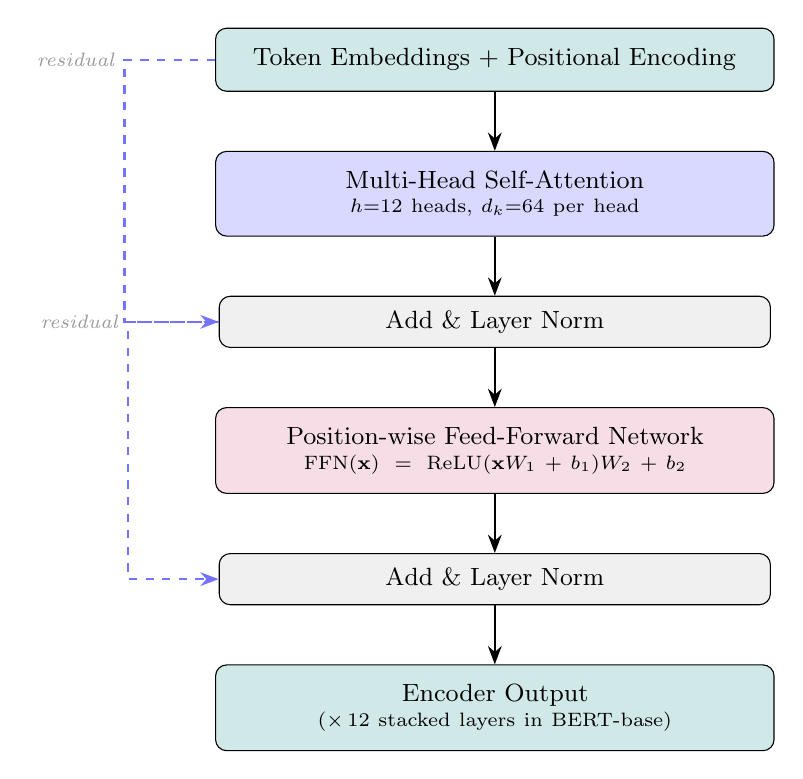
\begin{tikzpicture}[
  node distance=0.75cm,
  every node/.style={font=\small},
  mainbox/.style={draw, rounded corners=4pt, minimum width=7cm,
                  minimum height=0.80cm, fill=#1, align=center,
                  inner sep=7pt, text width=6.6cm},
  normbox/.style={draw, rounded corners=4pt, minimum width=7cm,
                  minimum height=0.65cm, fill=gray!12, align=center,
                  inner sep=5pt, font=\small},
  arr/.style ={->, >=Stealth, thick},
  skip/.style={->, >=Stealth, thick, dashed, blue!55}]

\node[mainbox=teal!18]   (embed) {Token Embeddings + Positional Encoding};
\node[mainbox=blue!15, below=of embed]  (mha)  {Multi-Head Self-Attention\\[-2pt]\scriptsize $h{=}12$ heads, $d_k{=}64$ per head};
\node[normbox,  below=of mha]           (ln1)  {Add \& Layer Norm};
\node[mainbox=purple!13, below=of ln1]  (ffn)  {Position-wise Feed-Forward Network\\[-2pt]\scriptsize $\mathrm{FFN}(\mathbf{x})=\mathrm{ReLU}(\mathbf{x}W_1+b_1)W_2+b_2$};
\node[normbox,  below=of ffn]           (ln2)  {Add \& Layer Norm};
\node[mainbox=teal!18, below=of ln2]    (outp) {Encoder Output\\[-2pt]\scriptsize ($\times\,12$ stacked layers in BERT-base)};

\draw[arr] (embed) -- (mha);
\draw[arr] (mha)   -- (ln1);
\draw[arr] (ln1)   -- (ffn);
\draw[arr] (ffn)   -- (ln2);
\draw[arr] (ln2)   -- (outp);

%% Residual connections (left rail, away from the main vertical flow)
\draw[skip] (embed.west) -- ++(-1.15,0)
    node[left, font=\scriptsize\itshape, text=gray!80] {residual}
    |- (ln1.west);
\draw[skip] (ln1.west) -- ++(-1.15,0)
    node[left, font=\scriptsize\itshape, text=gray!80] {residual}
    |- (ln2.west);
\end{tikzpicture}
\caption{Structure of a single transformer encoder layer as used in BERT and FinBERT.  Both the multi-head attention and feed-forward sub-layers are wrapped in a residual (skip) connection followed by layer normalisation, preserving gradient flow through the 12-layer stack.}
\label{fig:transformer_encoder}
\end{figure}

% ............................................................
\subsection{Positional Encoding}

Because the attention mechanism has no inherent sense of word order, position information
must be injected explicitly.
Vaswani et al.\ achieve this with a fixed encoding that uses sinusoidal functions of token
position $t$ and embedding dimension index $i$:
\begin{align}
  PE_{(t,\,2i)}   &= \sin\!\left(\frac{t}{10000^{2i/d_{\text{model}}}}\right) \\[4pt]
  PE_{(t,\,2i+1)} &= \cos\!\left(\frac{t}{10000^{2i/d_{\text{model}}}}\right)
\end{align}
where $d_{\text{model}} = 768$ in BERT-base.
The sinusoidal choice means that each position gets a unique, smoothly varying signature
across the embedding dimensions, and the model can learn to attend to relative positions
rather than absolute ones.
The positional encoding is added element-wise to the token embedding before the first
encoder layer.

% ............................................................
\subsection{Scaled Dot-Product Attention}

The central operation of the transformer is \emph{scaled dot-product attention}.
Inputs are projected into three matrices: queries $\mathbf{Q}$, keys $\mathbf{K}$,
and values $\mathbf{V}$. The output is a weighted sum of the values, where the
weights reflect how relevant each key is to each query:
\begin{equation}
  \text{Attention}(\mathbf{Q},\mathbf{K},\mathbf{V})
  = \text{softmax}\!\left(\frac{\mathbf{Q}\mathbf{K}^{\!\top}}{\sqrt{d_k}}\right)\mathbf{V}.
  \label{eq:attention}
\end{equation}

Each entry of $\mathbf{Q}\mathbf{K}^{\!\top}$ scores how strongly one position
attends to another.
After the softmax, each row becomes a probability distribution over all positions, and
multiplying by $\mathbf{V}$ produces a weighted average of value vectors.
The $\sqrt{d_k}$ scaling prevents the dot products from growing so large that the
softmax saturates into near-zero gradients, a practical issue that appeared
consistently in early training runs before scaling was introduced.

% ............................................................
\subsection{Multi-Head Attention}

Rather than applying one attention function to the full representation,
the transformer runs $h$ parallel \emph{attention heads}, each projecting into a separate
lower-dimensional subspace:
\begin{equation}
  \text{MultiHead}(\mathbf{Q},\mathbf{K},\mathbf{V})
  = \text{Concat}(\text{head}_1,\ldots,\text{head}_h)\,\mathbf{W}^O
  \label{eq:mha}
\end{equation}
where each $\text{head}_i = \text{Attention}(\mathbf{Q}\mathbf{W}_i^Q,\,
\mathbf{K}\mathbf{W}_i^K,\, \mathbf{V}\mathbf{W}_i^V)$ and the results are concatenated
and projected back via $\mathbf{W}^O$.
BERT-base uses $h = 12$ heads.

The motivation is that a single attention distribution must simultaneously resolve
multiple linguistic tasks.
Multiple heads allow the model to specialise: some learn local phrase-level dependencies,
others capture long-range entity references.
In financial text this matters because the sentiment-bearing term (e.g.\ ``surged'')
may appear several tokens away from the company name it modifies.

% ............................................................
\subsection{Feed-Forward Sub-layers and Residual Connections}

After the attention sub-layer, each encoder layer applies a two-layer feed-forward network
independently at every position:
\begin{equation}
  \text{FFN}(\mathbf{x}) = \max(0,\;\mathbf{x}\mathbf{W}_1 + \mathbf{b}_1)\,\mathbf{W}_2 + \mathbf{b}_2.
  \label{eq:ffn}
\end{equation}
Both the attention and FFN sub-layers are wrapped in a residual connection followed by
layer normalisation, which stabilises training across the 12-layer stack by preserving
a gradient path directly to earlier layers.

% ----------------------------------------------------------
\section{BERT and FinBERT}
% ----------------------------------------------------------

% ............................................................
\subsection{BERT Pre-training}

BERT \citep{devlin2019bert} pre-trains on two self-supervised objectives over large
unlabelled text corpora.

\textbf{Masked Language Modelling (MLM)} randomly selects 15\% of input tokens,
replacing 80\% of those with a \texttt{[MASK]} token, 10\% with a random vocabulary
token, and leaving 10\% unchanged.
The model is trained to predict the original token at each masked position from the
surrounding context.
The 10\%/10\% split is deliberate: if every selected token became \texttt{[MASK]},
the model would only learn to handle masked inputs, creating a mismatch at inference
time where \texttt{[MASK]} never appears.

\textbf{Next Sentence Prediction (NSP)} presents the model with pairs of sentences
and asks it to predict whether the second genuinely follows the first.
A special \texttt{[CLS]} token prepended to each input is used for the binary
classification.
RoBERTa \citep{liu2019roberta} later showed NSP to be unnecessary, but it is part of
the BERT setup that FinBERT inherits.

% ............................................................
\subsection{FinBERT Fine-tuning for Sentiment Classification}

Araci \citep{araci2019finbert} takes the pre-trained BERT-base weights, continues
pre-training on the Reuters TRC2 corpus and the Financial PhraseBank
\citep{malo2014financialphrasebank}, and then fine-tunes for three-class sentiment
classification (positive, neutral, negative).

Fine-tuning adds a single linear layer on top of the \texttt{[CLS]} token's final
representation $\mathbf{h}_{\texttt{[CLS]}}$:
\begin{equation}
  \hat{\mathbf{y}}
  = \text{softmax}\!\left(\mathbf{W}_c\,\mathbf{h}_{\texttt{[CLS]}} + \mathbf{b}_c\right),
  \label{eq:finbert_clf}
\end{equation}
where $\mathbf{W}_c \in \mathbb{R}^{3 \times 768}$.
Training minimises the standard cross-entropy loss between the predicted distribution
$\hat{\mathbf{y}}$ and the one-hot ground-truth label.

Domain pre-training matters because financial vocabulary is highly context-dependent.
The phrase ``the company cut its losses'' carries a positive connotation in a trading
context (implying a controlled exit), whereas a general-purpose model would classify
``cut'' and ``losses'' together as negative.
I chose FinBERT specifically because I needed financial understanding baked into the
representations before fine-tuning, not retrofitted afterwards.

% ----------------------------------------------------------
\section{Local Interpretable Model-Agnostic Explanations (LIME)}
% ----------------------------------------------------------

% ............................................................
\subsection{Core Idea}

LIME \citep{ribeiro2016lime} explains the prediction of any black-box model $f$ at a
specific input $x^*$ by fitting a simple, interpretable surrogate model in the local
neighbourhood of $x^*$.
Its \emph{model-agnostic} property means the same method applies regardless of whether
$f$ is FinBERT, a decision tree, or any other classifier
\citep{doshivelez2017interpretable}.  The end-to-end workflow is shown in Figure~\ref{fig:lime_process}.

\begin{figure}[H]
\centering
\resizebox{\textwidth}{!}{%
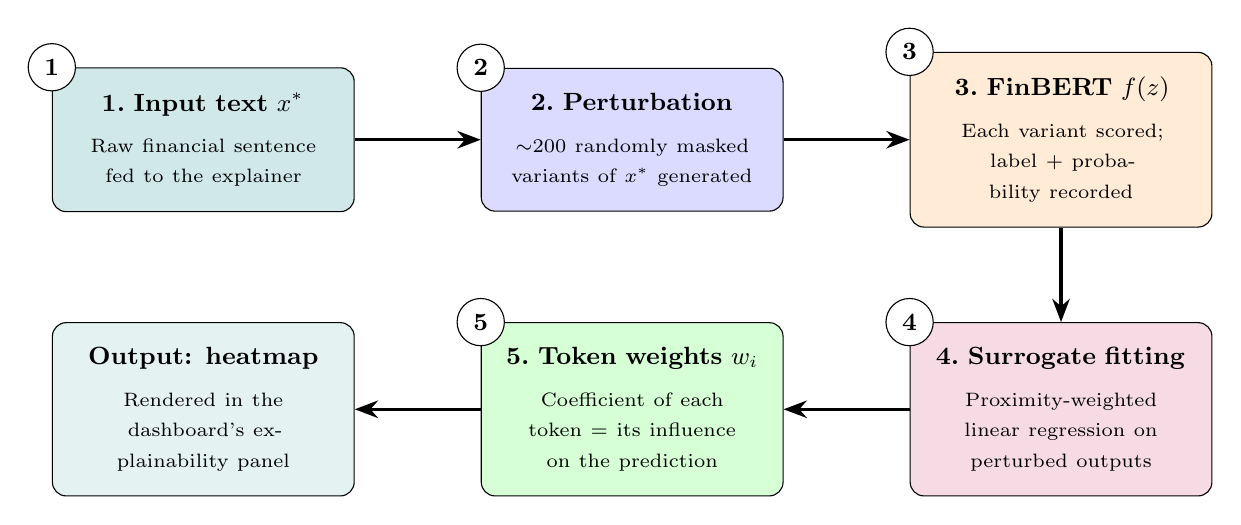
\begin{tikzpicture}[
  node distance=1.2cm and 1.6cm,
  every node/.style={font=\small},
  lmbox/.style={draw, rounded corners=5pt, fill=#1, minimum width=3.6cm,
                minimum height=1.5cm, align=center, inner sep=9pt,
                text width=3.2cm},
  num/.style={circle, draw, fill=white, minimum size=0.6cm,
              font=\small\bfseries, inner sep=0pt},
  arr/.style={->, >=Stealth, very thick, line width=1.2pt}]

%% Top row: steps 1–3
\node[lmbox=teal!18]   (input)   {\textbf{1.\ Input text} $x^*$\\[4pt]
  \scriptsize Raw financial sentence fed to the explainer};
\node[lmbox=blue!14,  right=of input]   (perturb) {\textbf{2.\ Perturbation}\\[4pt]
  \scriptsize $\sim$200 randomly masked variants of $x^*$ generated};
\node[lmbox=orange!16, right=of perturb] (query)   {\textbf{3.\ FinBERT} $f(z)$\\[4pt]
  \scriptsize Each variant scored; label + probability recorded};

%% Bottom row: steps 4–5 (right to left to form a U-shape)
\node[lmbox=purple!14, below=of query]   (fit)     {\textbf{4.\ Surrogate fitting}\\[4pt]
  \scriptsize Proximity-weighted linear regression on perturbed outputs};
\node[lmbox=green!16,  left=of fit]      (output)  {\textbf{5.\ Token weights} $w_i$\\[4pt]
  \scriptsize Coefficient of each token = its influence on the prediction};
\node[lmbox=teal!10,   left=of output]   (heatmap) {\textbf{Output: heatmap}\\[4pt]
  \scriptsize Rendered in the dashboard's explainability panel};

%% Step number badges – centred exactly on each box's north-west corner so the
%% disc straddles the corner (half inside / half outside) and never overlaps text.
\foreach \n/\nd in {1/input,2/perturb,3/query,4/fit,5/output}{
  \node[num] at (\nd.north west) {\n};
}

%% Arrows
\draw[arr] (input)   -- (perturb);
\draw[arr] (perturb) -- (query);
\draw[arr] (query)   -- (fit);
\draw[arr] (fit)     -- (output);
\draw[arr] (output)  -- (heatmap);
\end{tikzpicture}}
\caption{LIME explanation process applied to financial text classification.  The explainer generates perturbed variants of the input, queries the black-box FinBERT model on each, and fits a proximity-weighted linear surrogate to recover per-token importance weights.  These weights are displayed as a colour-coded heatmap in the dashboard.}
\label{fig:lime_process}
\end{figure}

% ............................................................
\subsection{The LIME Objective}

LIME searches for an interpretable model $g$ (here, a linear model) that balances
fidelity to $f$ locally against simplicity:
\begin{equation}
  \xi(x^*)
  = \arg\min_{g \;\in\; \mathcal{G}}
    \;\mathcal{L}(f,\,g,\,\pi_{x^*}) + \Omega(g)
  \label{eq:lime_obj}
\end{equation}
where $\mathcal{L}(f, g, \pi_{x^*})$ is the weighted prediction error between $f$ and $g$
over perturbed samples near $x^*$, $\Omega(g)$ penalises the complexity of $g$, and
$\pi_{x^*}(z) = \exp(-D(x^*, z)^2 / \sigma^2)$ is a proximity kernel that gives more
weight to samples close to $x^*$.

% ............................................................
\subsection{Perturbation and Surrogate Fitting for Text}

For a text input, LIME treats each word as a binary feature (present or absent).
It generates a set of perturbed versions of $x^*$ by randomly masking tokens, queries $f$
on each, and uses the resulting predictions as labels to fit the weighted linear surrogate.
The coefficients of the fitted model are token importance scores: a positive weight on a
word means that word pushed the prediction toward the target class; a negative weight means
it pushed against it.
This produces the token-level heatmap shown in the dashboard's explainability panel.

The key limitation is that a linear surrogate cannot capture non-local interactions,
for example negation that spans several tokens, which BERT's attention mechanism
handles naturally.
LIME's explanation is therefore an approximation of $f$'s behaviour near $x^*$, not a
global account of the model.
I accepted this trade-off because LIME's cost scales with the number of perturbations
sampled (around 200 for the text lengths I was working with), making it fast enough to
serve from a live API endpoint.

% ----------------------------------------------------------
\section{SHAP: SHapley Additive Explanations}
% ----------------------------------------------------------

% ............................................................
\subsection{Game-theoretic Foundation and the Shapley Value}

SHAP \citep{lundberg2017shap} grounds feature attribution in cooperative game theory.
Each feature $x_i$ is treated as a ``player'', and the model's output is the
``prize'' to be divided among the players.
The \emph{Shapley value} $\phi_i$ measures the average marginal contribution of feature
$i$ across all possible orderings in which features can be added to a coalition:
\begin{equation}
  \phi_i
  = \sum_{S \;\subseteq\; F \setminus \{i\}}
    \frac{|S|!\;(|F| - |S| - 1)!}{|F|!}
    \;\bigl[f(S \cup \{i\}) - f(S)\bigr]
  \label{eq:shapley}
\end{equation}
where $F$ is the full set of features, $S$ is a coalition not containing $i$,
$f(S)$ is the model's expected output given only the features in $S$, and the
combinatorial factor weights each coalition by how many orderings it corresponds to.

The Shapley value is the unique attribution that satisfies a set of fairness axioms,
including that attributions sum exactly to the model's output and that features with
equal contribution receive equal attribution.

% ............................................................
\subsection{Computational Cost and the Choice of LIME at Runtime}

Exactly evaluating~\eqref{eq:shapley} requires considering all $2^{|F|}$ subsets.
For a 128-token input this is entirely intractable.
KernelSHAP \citep{lundberg2017shap} approximates Shapley values by solving a
specially weighted regression, conceptually similar to LIME but with a different
kernel that is proven to recover the Shapley values in expectation.
Even with this approximation, a single SHAP explanation requires several hundred model
evaluations, versus LIME's $\sim$200 perturbations on comparable inputs.
This is the practical reason I served LIME from the real-time API and reserved SHAP
for offline notebook analysis.

% ----------------------------------------------------------
\section{Correlation and Causal Inference Methods}
% ----------------------------------------------------------

% ............................................................
\subsection{Pearson and Spearman Correlation}

Given two time series of length $T$, the Pearson correlation coefficient measures linear
co-movement:
\begin{equation}
  r = \frac{\sum_{t=1}^T (x_t - \bar{x})(y_t - \bar{y})}
           {\sqrt{\sum_{t=1}^T (x_t - \bar{x})^2}\;\;\sqrt{\sum_{t=1}^T (y_t - \bar{y})^2}},
  \label{eq:pearson}
\end{equation}
$r$ lies in $[-1, 1]$, with $+1$ indicating perfect positive linear co-movement.
Its limitation is that it assumes a bivariate normal distribution, which financial
returns do not satisfy (heavy tails, occasional extreme values).

Spearman's $r_s$ addresses this by applying the same formula to the \emph{ranks} of the
observations rather than the raw values, which removes distributional assumptions.
When there are no tied ranks it simplifies to:
\begin{equation}
  r_s = 1 - \frac{6\sum_{t=1}^T d_t^2}{T(T^2 - 1)},
  \label{eq:spearman}
\end{equation}
where $d_t$ is the difference in ranks of $x_t$ and $y_t$.
I report both measures so that the distance between them indicates how much of any
apparent relationship is an artefact of outliers or non-normality.

% ............................................................
\subsection{Rolling Window Correlation}

A single static correlation coefficient masks how the relationship changes over time;
for instance, sentiment--price coupling may strengthen during high-volatility periods and
weaken in calmer markets.
Rolling correlation applies the Pearson formula within a sliding window of width $W$,
producing a time series of coefficients $\{r_t^{(W)}\}$ that reveals these temporal
shifts.
I implemented this using \texttt{pandas.DataFrame.rolling().corr()} with a 30-day window,
which balanced responsiveness to regime changes against the noise introduced by short
windows.

% ............................................................
\subsection{Granger Causality}

Granger causality \citep{granger1969} asks: do past values of series $X$ improve
predictions of $Y$ beyond what $Y$'s own history alone provides?
It is important to note that this is \emph{predictive precedence}, not physical causation
in any deeper sense.

\paragraph{Stationarity.}
Both series must be stationary before the test is valid; non-stationary series can
generate spurious correlations \citep{engle1987cointegration}.
Sentiment scores are bounded and approximately stationary; stock prices are converted to
log-differenced returns $r_t = \log(P_t / P_{t-1})$ to remove the price trend.

\paragraph{Model comparison.}
For lag order $p$ (chosen by the Akaike Information Criterion), two autoregressive
models are fitted.
The \emph{unrestricted} model regresses $Y$ on its own past values and the past values
of $X$:
\begin{equation}
  y_t
  = \alpha_0
    + \sum_{k=1}^{p} \alpha_k\, y_{t-k}
    + \sum_{k=1}^{p} \beta_k\, x_{t-k}
    + \varepsilon_t.
  \label{eq:var_unrest}
\end{equation}
The \emph{restricted} model uses only $Y$'s own history:
\begin{equation}
  y_t
  = \alpha_0
    + \sum_{k=1}^{p} \alpha_k\, y_{t-k}
    + \varepsilon_t^R.
  \label{eq:var_rest}
\end{equation}

\paragraph{The F-test.}
The null hypothesis $H_0\colon \beta_1 = \cdots = \beta_p = 0$ is tested with:
\begin{equation}
  F = \frac{(RSS_R - RSS_U)\,/\,p}{RSS_U\,/\,(T - 2p - 1)}
  \;\sim\; F\!\left(p,\;T - 2p - 1\right),
  \label{eq:granger_f}
\end{equation}
where $RSS_R$ and $RSS_U$ are the residual sums of squares of the restricted and
unrestricted models.
A $p$-value below 0.05 means the added sentiment lags significantly reduce the
prediction error for returns, and $X$ is said to Granger-cause $Y$.

I found the results varied considerably by ticker.
Sentiment appeared to Granger-cause returns for some large-cap, news-driven equities
but showed no significant effect for others.
This is consistent with theory: more heavily traded, high-coverage stocks are more
sensitive to retail commentary than smaller or less liquid names where sentiment volume
is too low for the test to have power.
The inconsistency is itself a finding about which assets are most affected by public
sentiment.

% ----------------------------------------------------------
\section{Summary}
% ----------------------------------------------------------

This chapter has covered the theoretical basis for five method families used in the project.
The transformer's attention mechanism and FinBERT's domain pre-training explain why the
model performs well on financial text; LIME and SHAP each provide a principled route to
explaining individual predictions, with different cost and fidelity trade-offs; and
Pearson, Spearman, rolling correlation, and the Granger F-test together give a layered
view of the sentiment--price relationship that no single measure could provide alone.

Understanding these foundations directly shaped how I built and debugged the system.
Knowing that LIME approximates $f$ locally with a linear model, for instance, helped me
interpret cases where the token heatmap contradicted my intuition, and the disagreement was
not a bug in my code but a consequence of the linear surrogate breaking down in a
non-linear region of the decision boundary.
The next chapter describes how these methods were combined into a working system.

\chapter{System Design and Methodology}
\label{chap:system_design}

This chapter describes the design decisions behind the \textit{Investor Sentiment Dashboard} and the reasoning that led to them. I cover the system architecture, ethical considerations, requirements, data collection strategy, preprocessing approach, and modelling choices that underpin the implementation described in Chapter~\ref{chap:implementation}. Where relevant I explain not just what I decided, but why.

\section{System Overview}
\label{sec:system_overview}

I designed the system around a modular five-tier architecture, illustrated in Figure~\ref{fig:system_architecture}: (1)~\textit{data ingestion}, (2)~\textit{NLP processing and enrichment}, (3)~\textit{storage and entity resolution}, (4)~\textit{REST API}, and (5)~\textit{interactive frontend}. The reason for this layered structure was to keep computationally intensive inference components separate from the API serving layer, so that each tier could be developed, tested, and deployed independently.

\begin{figure}[H]
\centering
\resizebox{\textwidth}{!}{%
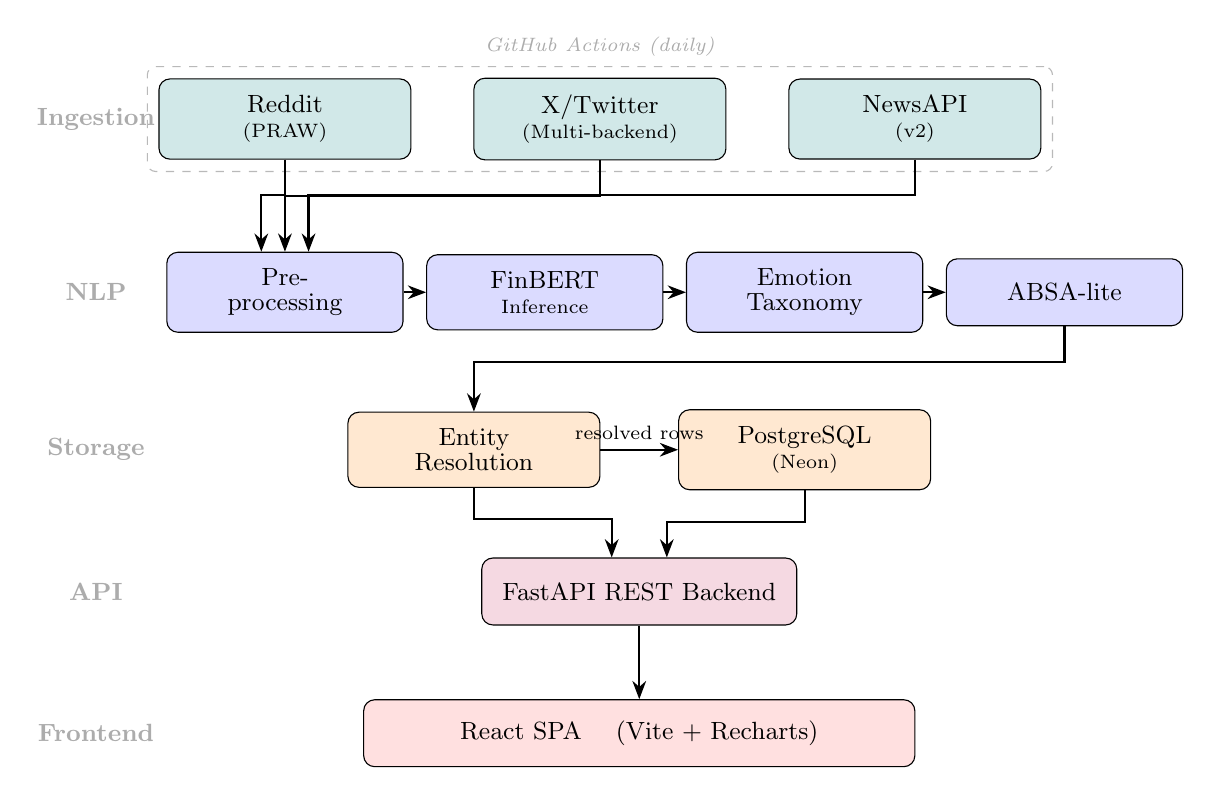
\begin{tikzpicture}[
  every node/.style={font=\small},
  src/.style  ={draw, rounded corners=4pt, minimum width=3.2cm, minimum height=0.85cm,
                fill=teal!18, align=center, inner sep=6pt},
  proc/.style ={draw, rounded corners=4pt, minimum width=3.0cm, minimum height=0.85cm,
                fill=blue!14, align=center, inner sep=6pt},
  stor/.style ={draw, rounded corners=4pt, minimum width=3.2cm, minimum height=0.85cm,
                fill=orange!18, align=center, inner sep=6pt},
  apist/.style={draw, rounded corners=4pt, minimum width=4.0cm, minimum height=0.85cm,
                fill=purple!15, align=center, inner sep=6pt},
  front/.style={draw, rounded corners=4pt, minimum width=7.0cm, minimum height=0.85cm,
                fill=red!12, align=center, inner sep=6pt},
  lbl/.style  ={font=\small\bfseries, text=gray!65},
  arr/.style  ={->, >=Stealth, thick},
  darr/.style ={draw, dashed, gray!55, rounded corners=3pt}]

%% ── Tier labels (left column) ────────────────────────────────────
\node[lbl] at (-2.4,  0.0) {Ingestion};
\node[lbl] at (-2.4, -2.2) {NLP};
\node[lbl] at (-2.4, -4.2) {Storage};
\node[lbl] at (-2.4, -6.0) {API};
\node[lbl] at (-2.4, -7.8) {Frontend};

%% ── Tier 1: Ingestion ─────────────────────────────────────────────
\node[src] (reddit)  at (0.0,  0.0) {Reddit\\[-2pt]\scriptsize (PRAW)};
\node[src] (twitter) at (4.0,  0.0) {X/Twitter\\[-2pt]\scriptsize (Multi-backend)};
\node[src] (newsapi) at (8.0,  0.0) {NewsAPI\\[-2pt]\scriptsize (v2)};

%% ── Tier 2: NLP Pipeline ─────────────────────────────────────────
\node[proc] (preproc) at (0.0, -2.2) {Pre-\\[-2pt]processing};
\node[proc] (finbert) at (3.3, -2.2) {FinBERT\\[-2pt]\scriptsize Inference};
\node[proc] (taxon)   at (6.6, -2.2) {Emotion\\[-2pt]Taxonomy};
\node[proc] (absa)    at (9.9, -2.2) {ABSA-lite};

%% ── Tier 3: Storage ──────────────────────────────────────────────
\node[stor] (entity)  at (2.4, -4.2) {Entity\\[-2pt]Resolution};
\node[stor] (db)      at (6.6, -4.2) {PostgreSQL\\[-2pt]\scriptsize (Neon)};

%% ── Tier 4: API ──────────────────────────────────────────────────
\node[apist] (api)    at (4.5, -6.0) {FastAPI REST Backend};

%% ── Tier 5: Frontend ─────────────────────────────────────────────
\node[front] (front)  at (4.5, -7.8) {React SPA \quad (Vite + Recharts)};

%% ── GitHub Actions dashed frame ──────────────────────────────────
\node[darr, fit=(reddit)(twitter)(newsapi), inner sep=4pt,
      label={[font=\scriptsize\itshape, text=gray!65]above:GitHub Actions (daily)}] (ghframe) {};

%% ── Arrows T1 → T2 (staggered entry points so arrows don't stack on one spot) ──
\draw[arr] (reddit.south)  -- ++(0,-0.45) -| ($(preproc.north)+(-0.30,0)$);
\draw[arr] (twitter.south) -- ++(0,-0.45) -| (preproc.north);
\draw[arr] (newsapi.south) -- ++(0,-0.45) -| ($(preproc.north)+(+0.30,0)$);

%% ── Arrows within T2 (processing chain) ─────────────────────────
\draw[arr] (preproc) -- (finbert);
\draw[arr] (finbert) -- (taxon);
\draw[arr] (taxon)   -- (absa);

%% ── Arrows T2 → T3 (NLP output → entity resolution → database) ──
\draw[arr] (absa.south) -- ++(0,-0.45) -| (entity.north);
\draw[arr] (entity.east) -- node[above, font=\scriptsize]{resolved rows} (db.west);

%% ── Arrows T3 → T4 (split entry points to avoid overlap) ────────
\draw[arr] (entity.south) -- ++(0,-0.4) -| ($(api.north)+(-0.35,0)$);
\draw[arr] (db.south)     -- ++(0,-0.4) -| ($(api.north)+(+0.35,0)$);

%% ── Arrows T4 → T5 ───────────────────────────────────────────────
\draw[arr] (api) -- (front);
\end{tikzpicture}}
\caption{Five-tier system architecture of the Investor Sentiment Dashboard.  Ingested records from Reddit, X/Twitter, and NewsAPI all enter the same preprocessing and NLP chain (FinBERT, emotion taxonomy, ABSA), then pass through entity resolution before being written to PostgreSQL.  The REST API and React SPA sit above storage.  The dashed border marks ingestion components scheduled by the daily GitHub Actions workflow.}
\label{fig:system_architecture}
\end{figure}

I collect text from three sources (Reddit, X/Twitter, and financial news) through dedicated pipelines that each handle their own rate limits and authentication. Each pipeline feeds into a shared preprocessing and FinBERT inference layer, after which the finance-emotion taxonomy and ABSA module enrich each record. A stock entity resolution layer then maps free-text mentions to canonical ticker symbols. Processed records go into a cloud PostgreSQL database (Neon), and a FastAPI backend serves aggregate statistics, per-ticker sentiment, LIME explanations, and correlation results to the React frontend. I automated daily collection using GitHub Actions so the corpus continues to grow without manual intervention.

\section{Development Methodology and Project Management}
\label{sec:dev_methodology}

\subsection{Development Approach}

I used an iterative, sprint-based approach rather than a strict waterfall model. I chose this for three practical reasons. First, my research questions were still being refined during the literature review, which made it impractical to lock down all requirements at the start. Second, each technical component had a clear dependency on the previous one: I could not build the API before the inference engine, and could not build the frontend before the API, so iterating through them in sequence made sense. Third, an iterative approach meant each completed sprint produced something I could write up immediately, which made the concurrent dissertation writing much more manageable.

\subsection{Project Tracking and Tooling}

I tracked progress at two levels. At the strategic level, I produced a Gantt chart (Appendix~\ref{app:gantt}) covering 31 August 2025 to 21 April 2026 across ten phases, included in my approved Project Brief in October 2025. At the tactical level, a Jira board decomposed each Gantt phase into individual tasks with unique identifiers. For example, the Data Collection \& Preprocessing phase (FYP-126) was broken into sub-tasks for PRAW integration, the multi-backend Twitter pipeline, NewsAPI setup, and the preprocessing module. The Sentiment Model phase (FYP-127) covered model setup, batch inference, error handling, and the preprocessing configuration in Listing~\ref{lst:finbert_config}.

I reviewed and updated the Gantt at the January 2026 deliverable milestone. The first three phases had completed on schedule. The Sentiment Model phase had started slightly later than I originally targeted, because I had spent extra time on the NewsAPI robustness issues described in Chapter~\ref{chap:implementation}. That did not affect the overall schedule, but it reinforced for me that the data ingestion layer needs more time than it looks like it will.

\subsection{Scope Management}

I did not cut any planned objectives, but the scope grew in two ways I had not anticipated. The Twitter ingestion grew from a single Tweepy implementation into a three-backend architecture because the official API rate limits turned out to be far more restrictive than I had planned for. That expansion is described in detail in Section~\ref{sec:data_ingestion}. The correlation module also grew: I originally planned a simple Pearson correlation display, but reading the literature made it clear that a single coefficient is insufficient for financial time-series, so I extended it to include Spearman, lag analysis, Granger causality, rolling correlation, and market adjustment. Both expansions were absorbed into existing sprints without changing the high-level Gantt.

\section{Ethical Considerations and Data Governance}
\label{sec:ethics}

Collecting data from social media and news outlets requires careful attention to ethical guidelines and platform terms of service. I restricted all data collection to publicly available text; the system does not access private communications, protected user data, or paywalled content. The completed Ethics Awareness Form was submitted with the approved Project Brief (October 2025); Appendix~\ref{app:ethics} explains where that signed form lives relative to this dissertation so it is not duplicated here.

\subsection{Platform Terms of Service and API Compliance}

Reddit data is collected using the Python Reddit API Wrapper (PRAW) with OAuth2 authentication, operating strictly within Reddit's published developer terms.  Rate limits are respected through automatic pagination and exponential backoff handling.  X/Twitter data is collected via the \texttt{snscrape} library by default, which accesses publicly available posts through the same pathway as the web interface.  Where an official API bearer token is configured, the system switches to Tweepy's X API v2 client, enforcing v2 rate limits automatically.  The system also supports a historical CSV ingestion backend to enable reproducible evaluation using pre-collected datasets.  NewsAPI data is retrieved through a registered developer account using the documented API interface.

All pipelines implement rate-limit resilience through exponential backoff and configurable per-run quotas, preventing any risk of service disruption or account suspension.

\subsection{Anonymisation and Storage}

To protect individual privacy, I strip personally identifiable information (user handles, display names, and geolocation metadata) during ingestion and preprocessing. Each stored record contains only sanitised text, a timestamp, a source identifier, and any extracted ticker mentions. The database is accessible only through project-specific credentials and is used solely for academic research, in compliance with the Loughborough University ethical policy framework \citep{lboro_ethics}.

\section{Requirements Analysis}
\label{sec:requirements_analysis}

I derived the system requirements from four sources: the gaps identified in my literature review, analysis of what existing sentiment tools do and do not provide, reflection on what the project needed to achieve its research objectives, and three structured expert interviews (two on 13 October 2025 and one on 21 October 2025) conducted during the project setup phase.

During October 2025, I conducted these interviews with finance and technology practitioners to understand how sentiment data is used in practice and what analytical capabilities a dashboard would need to be genuinely useful.  Three themes emerged consistently: practitioners wanted per-source sentiment comparisons (not just an aggregate), they wanted some basis for trusting an automated sentiment label, and they were interested in correlating sentiment signals with price data.  These interviews directly influenced the decision to prioritise the per-source filtering interface, the LIME explainability endpoint, and the full-featured correlation engine.  A summary of the interviews is provided in Appendix~\ref{app:interviews}.

\subsection{Functional Requirements}

\begin{itemize}
    \item Collect and preprocess text data from Reddit, X/Twitter, and financial news, with resilient multi-backend support for X.
    \item Perform financial sentiment classification using FinBERT, producing a three-class label and per-class probability distribution.
    \item Enrich FinBERT outputs with a finance-specific emotion label and score distribution (fear, optimism, uncertainty, confidence, scepticism, mixed).
    \item Extract aspect-tagged evidence sentences for six financial aspect categories (ABSA-lite).
    \item Resolve free-text stock and company mentions to canonical ticker symbols using NER and fuzzy matching.
    \item Generate LIME token-level explanations via a dedicated REST endpoint, renderable in the frontend.
    \item Persist all records to a relational database and expose aggregate statistics, per-ticker time-series, and data quality metrics via a versioned REST API.
    \item Compute and expose Pearson, Spearman, lag, Granger causality, and rolling correlation between sentiment and real-time asset prices.
    \item Provide an interactive React SPA with Market Overview and Stock Analysis views, plus Methodology and Legal pages.
    \item Support a lean deployment mode in which computationally heavy components return graceful 503 responses rather than failing.
\end{itemize}

\subsection{Non-Functional Requirements}

\begin{itemize}
    \item \textbf{Performance:}  Standard API data endpoints should respond within 3~seconds; LIME explanations, which involve a CPU-bound background computation, are exempt and may take up to 120~seconds.
    \item \textbf{Scalability:}  The system must support integration of new data sources, models, or asset classes without restructuring the core API.
    \item \textbf{Reproducibility:}  All ingestion, preprocessing, and evaluation scripts must produce deterministic outputs from the same input; random states are fixed throughout.
    \item \textbf{Usability:}  Dashboard visualisations must remain interpretable to a non-specialist financial audience; methodology and limitations must be prominently documented within the application.
    \item \textbf{Security:}  Production deployments must use API key authentication and security headers; credentials are managed via environment variables and never committed to version control.
    \item \textbf{Ethics:}  All data collection must comply with platform terms of service and the university ethical policy~\citep{lboro_ethics}.
\end{itemize}

\section{Data Collection and Preprocessing}
\label{sec:data_collection}

\subsection{Multi-Source Strategy and Rationale}

One of my central aims was to aggregate sentiment from multiple online environments rather than relying on a single source. My reading of the literature made it clear that any single platform gives you a biased picture: social media captures short-term emotional reactions, financial news is more institutional and structured, and Reddit retail communities can diverge sharply from both \citep{tetlock2007giving, bollen2011twitter, long2023reddit, schumaker2009textmining}. I decided to collect from three complementary sources to mitigate those individual biases:

\begin{itemize}
    \item \textbf{Reddit} contributes long-form, discussion-driven sentiment from finance-oriented subreddits (e.g., r/stocks, r/investing, r/cryptocurrency).  Posts include justifications, counter-arguments, and structured analysis of market events, enriching the sentiment signal with contextual depth.
    \item \textbf{X/Twitter} provides high-frequency short messages reacting to intraday price movements, earnings releases, and breaking news \citep{bollen2011twitter}, capturing rapid retail sentiment shifts that may precede news articles.
    \item \textbf{Financial news} adds contextualised, professionally sourced text from outlets including Reuters and Bloomberg via NewsAPI, providing a lower-noise reference signal against which social media sentiment can be compared.
\end{itemize}

\subsection{Preprocessing Pipeline}

Online text from these sources is inherently heterogeneous and noisy.  A standardised offline preprocessing pipeline, depicted in Figure~\ref{fig:preprocessing-pipeline}, transforms raw multi-source text into clean, model-ready inputs.

\begin{figure}[ht]
\centering
\begin{tikzpicture}[
  node distance=0.5cm,
  flowbox/.style={draw, rounded corners=4pt, minimum width=10cm,
                  minimum height=0.80cm, text width=9.4cm,
                  fill=blue!10, align=left, inner sep=8pt, font=\small},
  io/.style    ={draw, rounded corners=4pt, minimum width=10cm,
                  minimum height=0.80cm, text width=9.4cm,
                  fill=teal!18, align=center, font=\small\bfseries},
  arr/.style   ={->, >=Stealth, thick}]

\node[io]  (input)  {Raw Multi-source Text (Reddit post / Tweet / News article)};
\node[flowbox, below=of input]  (clean)  {\textbf{Step 1:} URL, HTML tag, and emoji removal};
\node[flowbox, below=of clean]  (case)   {\textbf{Step 2:} Case preservation (\texttt{lowercase: False}), retaining ticker symbols};
\node[flowbox, below=of case]   (negat)  {\textbf{Step 3:} Negation rewriting (\texttt{"not profitable"} $\to$ negation prefix token)};
\node[flowbox, below=of negat]  (punct)  {\textbf{Step 4:} Financial punctuation preserved (\%, \$, decimal separators left intact)};
\node[flowbox, below=of punct]  (stop)   {\textbf{Step 5:} Stopwords retained, as full sentence structure is needed for attention};
\node[flowbox, below=of stop]   (meta)   {\textbf{Step 6:} Source identifier and timestamp stored alongside the cleaned text};
\node[io,  below=of meta]  (output) {FinBERT-ready token sequence + structured record $\to$ PostgreSQL};

\draw[arr] (input)  -- (clean);
\draw[arr] (clean)  -- (case);
\draw[arr] (case)   -- (negat);
\draw[arr] (negat)  -- (punct);
\draw[arr] (punct)  -- (stop);
\draw[arr] (stop)   -- (meta);
\draw[arr] (meta)   -- (output);
\end{tikzpicture}
\caption{Offline preprocessing pipeline transforming raw multi-source financial text into structured, model-ready inputs.  All six steps are applied under the \texttt{finbert} configuration; lighter configurations (\texttt{minimal}, \texttt{standard}) omit or relax selected steps for non-transformer use cases.}
\label{fig:preprocessing-pipeline}
\end{figure}

The pipeline applies a \textbf{source-specific configuration} determined by the \texttt{config} parameter passed to the preprocessing script.  Four named configurations are provided (\texttt{minimal}, \texttt{standard}, \texttt{full}, \texttt{finbert}); all sentiment inference uses the \texttt{finbert} configuration, which is specifically tuned for transformer input:

\begin{itemize}
    \item \textbf{Case preservation} (\texttt{lowercase: False}): FinBERT's vocabulary retains case sensitivity important for ticker symbols and proper nouns.
    \item \textbf{URL and HTML removal} (\texttt{remove\_urls: True}): links and markup tokens contribute no semantic signal.
    \item \textbf{Stopword retention} (\texttt{remove\_stopwords: False}): FinBERT is trained on full sentences; removing common words degrades attention patterns \citep{araci2019finbert}.
    \item \textbf{No lemmatisation} (\texttt{lemmatize: False}): transformers use subword tokenisation and understand morphological variants directly.
    \item \textbf{Financial punctuation preservation} (\path{preserve_financial_punctuation: True}): percentage signs, dollar symbols, and decimal separators carry semantic weight in financial text.
    \item \textbf{Negation handling} (\texttt{handle\_negations: True}): phrases such as ``not profitable'' are rewritten to prevent polarity inversion in downstream classification.
\end{itemize}

Text fields processed per source are determined by a source-field mapping (\path{SOURCE_TEXT_FIELDS}), ensuring that Reddit post titles, Twitter post bodies, and NewsAPI article descriptions are each extracted from the correct JSON field before entering the shared cleaning pipeline.

All cleaned records are stored in the database with both raw and cleaned text preserved, ensuring full reproducibility and the ability to reprocess data under alternative configurations without re-ingestion.

\subsection{Data Quality and Deduplication}

Duplicate detection applies content-hash comparison at ingestion time to avoid counting the same post or article multiple times.  Near-duplicate detection using TF-IDF cosine similarity removes paraphrased or lightly edited reposts.  Minimum content length thresholds are enforced to exclude noise artefacts (e.g., single-emoji posts).

\section{Model Design}
\label{sec:model_design}

\subsection{Sentiment Classification: FinBERT}

I chose FinBERT \citep{araci2019finbert} as the core classifier because it is domain-adaptively pre-trained on financial corpora, giving it a well-documented advantage over general-purpose models on finance-specific benchmarks \citep{malo2014financialphrasebank}. The model is loaded from the \texttt{ProsusAI/finbert} checkpoint via the Hugging Face \texttt{transformers} library \citep{wolf2020transformers} and used in zero-shot inference mode (no further fine-tuning), classifying text as \textit{positive}, \textit{neutral}, or \textit{negative} with associated probability scores. I chose to preserve the full probability distribution rather than just the label, because those scores feed directly into the emotion taxonomy and entropy calculation downstream.

\subsection{Keyword Baseline}

A keyword-based sentiment classifier using domain-specific financial vocabulary is maintained as a lightweight baseline.  This enables a formal comparative evaluation (see Chapter~\ref{chap:evaluation}) and provides a fast fallback in contexts where transformer inference is unavailable.

\subsection{Novel: Finance-Emotion Taxonomy}
\label{sec:emotion_design}

The idea for the finance-emotion taxonomy came from noticing, during early testing, that FinBERT's three-class output was losing a lot of nuance that actually mattered. An investor expressing fear about a debt downgrade and an investor expressing scepticism about an overvalued growth stock both receive a ``negative'' label, but these are fundamentally different market signals. I designed the taxonomy to capture that distinction.  The taxonomy defines six domain emotions: \textit{fear}, \textit{optimism}, \textit{uncertainty}, \textit{confidence}, \textit{scepticism}, and \textit{mixed}.  These categories are grounded in prior behavioural finance research on investor mood states \citep{bollen2011twitter} and the lexical patterns that characterise different investor postures in financial text.

The emotion inference engine receives FinBERT's softmax probability vector, a normalised Shannon entropy score (measuring the model's decisiveness), a set of aspect evidence snippets, and performs the following steps:
\begin{enumerate}
    \item Initialises base scores for each emotion from configurable priors.
    \item Applies FinBERT probability-weighted increments: positive probability contributes to optimism and confidence; negative to fear and scepticism; neutral to uncertainty, weighted by entropy.
    \item Applies domain lexicon matching, incrementing scores for each matched phrase from a curated finance lexicon covering each emotion category.
    \item Applies aspect priors: each detected financial aspect (e.g., \texttt{risk\_liquidity}, \texttt{valuation}) contributes emotion-specific bonuses calibrated to the aspect's typical sentiment implications.
    \item Normalises scores to a probability simplex and selects the dominant emotion; if the top score is insufficiently differentiated or entropy is high, the result defaults to \textit{mixed}.
\end{enumerate}

This architecture is novel in that it combines model-derived probabilistic signals, entropy-based uncertainty quantification, and lexical domain knowledge within a single unified scoring function, without requiring any labelled training data for the emotion layer itself.  Figure~\ref{fig:emotion_taxonomy} illustrates the inference logic.

\begin{figure}[H]
\centering
\resizebox{\textwidth}{!}{%
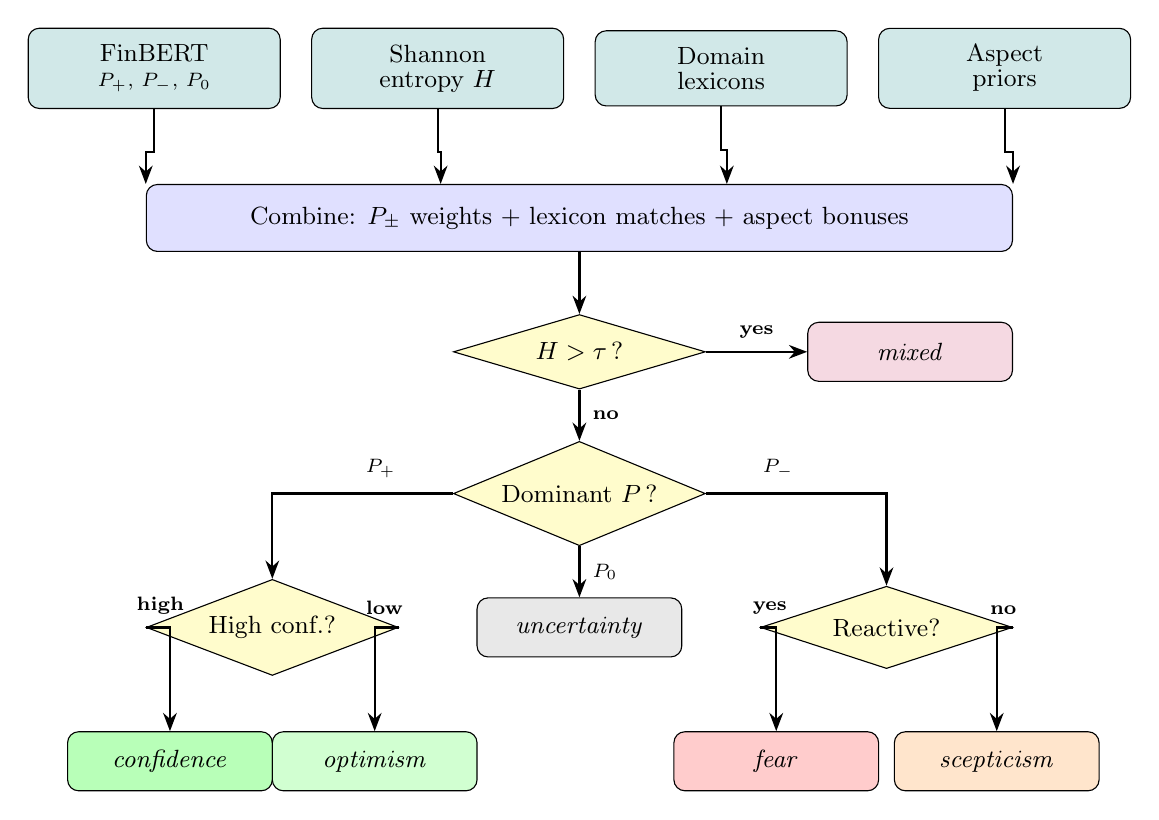
\begin{tikzpicture}[
  every node/.style={font=\small},
  inpbox/.style={draw, rounded corners=4pt, fill=teal!18,
                 minimum width=3.2cm, minimum height=0.85cm,
                 align=center, inner sep=6pt},
  procbox/.style={draw, rounded corners=4pt, fill=blue!12,
                  minimum width=11cm, minimum height=0.85cm,
                  align=center, inner sep=6pt},
  dec/.style   ={draw, diamond, fill=yellow!20, aspect=2.2,
                 minimum width=3.2cm, minimum height=0.75cm,
                 align=center, inner sep=2pt},
  outbox/.style={draw, rounded corners=4pt, minimum width=2.6cm,
                 minimum height=0.75cm, align=center, inner sep=5pt},
  arr/.style   ={->, >=Stealth, thick},
  labl/.style  ={font=\scriptsize\bfseries}]

%% ── Row 1: Four inputs ───────────────────────────────────────────
\node[inpbox] (finbert) at (0,   0) {FinBERT\\[-2pt]\scriptsize$P_+,\,P_-,\,P_0$};
\node[inpbox] (entropy) at (3.6, 0) {Shannon\\[-2pt]entropy $H$};
\node[inpbox] (lexicon) at (7.2, 0) {Domain\\[-2pt]lexicons};
\node[inpbox] (aspects) at (10.8,0) {Aspect\\[-2pt]priors};

%% ── Row 2: Scoring ───────────────────────────────────────────────
\node[procbox] (score)  at (5.4,-1.9) {Combine: $P_\pm$ weights + lexicon matches + aspect bonuses};

%% ── Row 3: High entropy decision ─────────────────────────────────
\node[dec] (hiH)   at (5.4, -3.6) {$H > \tau$\,?};
\node[outbox, fill=purple!15] (mixed) at (9.6, -3.6) {\textit{mixed}};

%% ── Row 4: Dominant polarity decision ────────────────────────────
\node[dec] (dom)   at (5.4, -5.4) {Dominant $P$\,?};

%% ── Row 5: Sub-decisions ─────────────────────────────────────────
\node[dec] (highP) at (1.5, -7.1) {High conf.?};
\node[outbox, fill=gray!18]   (unc)  at (5.4, -7.1) {\textit{uncertainty}};
\node[dec] (highN) at (9.3, -7.1) {Reactive?};

%% ── Row 6: Output labels ─────────────────────────────────────────
\node[outbox, fill=green!28] (conf)  at (0.2, -8.8) {\textit{confidence}};
\node[outbox, fill=green!18] (opt)   at (2.8, -8.8) {\textit{optimism}};
\node[outbox, fill=red!20]   (fear)  at (7.9, -8.8) {\textit{fear}};
\node[outbox, fill=orange!20](skep)  at (10.7,-8.8) {\textit{scepticism}};

%% ── Arrows: inputs → scoring (split anchors so lines do not stack) ──
\draw[arr] (finbert.south) -- ++(0,-0.55) -| (score.north west);
\draw[arr] (entropy.south) -- ++(0,-0.55) -| ($(score.north west)!0.34!(score.north east)$);
\draw[arr] (lexicon.south) -- ++(0,-0.55) -| ($(score.north west)!0.67!(score.north east)$);
\draw[arr] (aspects.south) -- ++(0,-0.55) -| (score.north east);

%% ── Arrows: scoring → hiH → dom ─────────────────────────────────
\draw[arr] (score) -- (hiH);
\draw[arr] (hiH.east)  -- node[labl, above=1pt]{yes} (mixed.west);
\draw[arr] (hiH.south) -- node[labl, right=1pt]{no}  (dom.north);

%% ── Arrows: dom → three branches ─────────────────────────────────
\draw[arr] (dom.west)  -| node[labl, above=2pt, pos=0.2]{$P_+$} (highP.north);
\draw[arr] (dom.south) -- node[labl, right=1pt]{$P_0$}           (unc.north);
\draw[arr] (dom.east)  -| node[labl, above=2pt, pos=0.2]{$P_-$} (highN.north);

%% ── Positive branch ──────────────────────────────────────────────
\draw[arr] (highP.west) -| node[labl, above=1pt, pos=0.3]{high} (conf.north);
\draw[arr] (highP.east) -| node[labl, above=1pt, pos=0.3]{low}  (opt.north);

%% ── Negative branch ──────────────────────────────────────────────
\draw[arr] (highN.west) -| node[labl, above=1pt, pos=0.3]{yes}  (fear.north);
\draw[arr] (highN.east) -| node[labl, above=1pt, pos=0.3]{no}   (skep.north);
\end{tikzpicture}}
\caption{Finance-emotion taxonomy inference logic.  FinBERT's softmax probability vector, Shannon entropy, domain lexicon scores, and aspect priors are combined into per-emotion scores.  High entropy triggers a \textit{mixed} assignment; otherwise the dominant polarity determines the branch, with further subdivision based on confidence level (positive branch) or reactivity (negative branch).}
\label{fig:emotion_taxonomy}
\end{figure}

\subsection{Novel: Lightweight ABSA Module}
\label{sec:absa_design}

To provide traceable justification for sentiment scores, the system implements a lightweight Aspect-Based Sentiment Analysis (ABSA) module \citep{pontiki2014semeval} that operates without fine-tuned sequence models.  Sentences in each document are segmented and matched against six financial aspect keyword buckets:

\begin{itemize}
    \item \textbf{revenue\_earnings}: profit, EPS, guidance, margin, beat/miss estimates.
    \item \textbf{growth\_demand}: subscriber growth, capacity, adoption, expansion.
    \item \textbf{risk\_liquidity}: debt, bankruptcy, SEC investigation, writedown.
    \item \textbf{valuation}: P/E ratio, price target, overvalued/undervalued.
    \item \textbf{product\_ai}: product launch, AI, GPU, innovation, patent.
    \item \textbf{macro\_policy}: Fed rates, inflation, tariffs, stimulus.
\end{itemize}

Matched sentences are returned as tagged evidence snippets with their aspect category and, optionally, a per-snippet FinBERT label.  This lightweight design provides interpretable, aspect-grounded justifications for the headline sentiment label while remaining computationally tractable in high-throughput pipelines, an important practical constraint identified in the system requirements.

\section{Explainability Integration}
\label{sec:explainability_design}

LIME \citep{ribeiro2016lime} is integrated as the primary user-facing explainability method.  For each sentiment prediction, LIME generates token-level importance weights by systematically perturbing the input text and fitting a local linear surrogate model.  The resulting weights are returned via a dedicated REST endpoint and rendered as an interactive token-level heatmap in the frontend's Stock Analysis page.

SHAP \citep{lundberg2017shap} is implemented within the backend's explainability module and is accessible via the API for offline auditing and corpus-level analysis.  Given its substantially higher computational cost, SHAP is not exposed in the live frontend but is used in research notebooks and for generating summary importance statistics.

I chose LIME for real-time API responses and reserved SHAP for offline analysis. The trade-off here is theoretical rigour (SHAP) versus practical latency (LIME), and the literature on deployable XAI supports that decision \citep{yeo2023xai}. SHAP's computational cost would have made it impossible to serve interactively from a cloud instance with realistic resource constraints.

\section{Stock Entity Resolution}
\label{sec:entity_design}

To enable per-ticker analytics, a stock entity resolution pipeline links free-text mentions to canonical ticker symbols using a three-stage process:
\begin{enumerate}
    \item \textbf{Named Entity Recognition (NER)}: spaCy's \texttt{en\_core\_web\_sm} model extracts \texttt{ORG}, \texttt{PRODUCT}, and \texttt{GPE} entities from cleaned text.
    \item \textbf{Exact matching}: extracted entity strings are compared against a curated stock database of ticker symbols and company names.
    \item \textbf{Fuzzy matching}: entities not resolved by exact match are compared using the FuzzyWuzzy library's partial ratio scorer with a configurable similarity threshold (default 0.85), allowing resolution of common abbreviations and partial names.
\end{enumerate}

A curated blacklist prevents common false positives (``Fed'', ``SEC'', ``White House'') from being incorrectly resolved to tickers.  The three-stage pipeline is summarised in Figure~\ref{fig:entity_resolution}.

\begin{figure}[H]
\centering
\resizebox{\textwidth}{!}{%
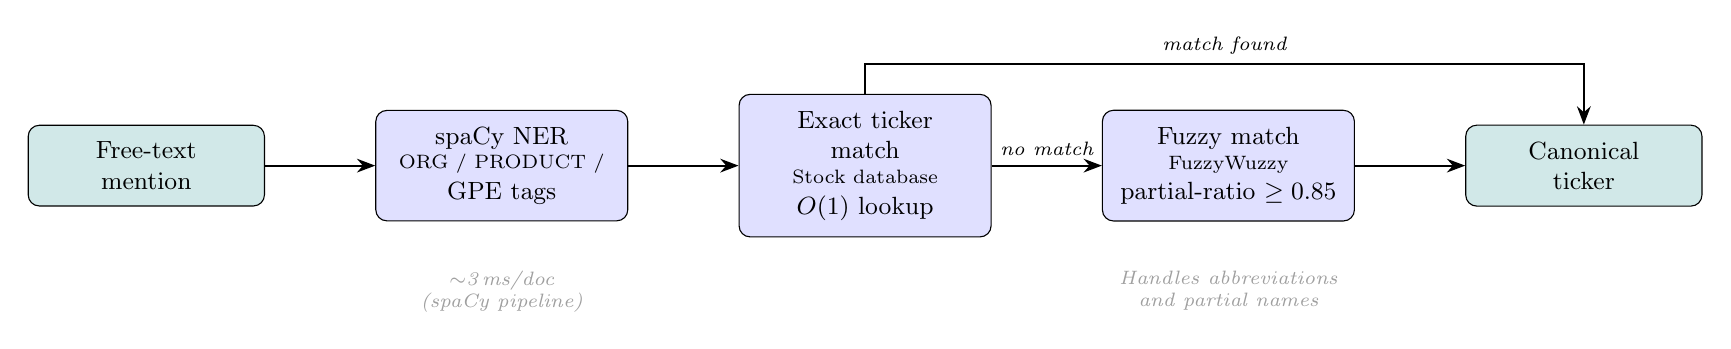
\begin{tikzpicture}[
  node distance=0.6cm and 1.4cm,
  every node/.style={font=\small},
  io/.style  ={draw, rounded corners=4pt, fill=teal!18, minimum width=3.0cm,
               minimum height=0.85cm, align=center, inner sep=6pt},
  ebox/.style={draw, rounded corners=4pt, fill=blue!12, minimum width=3.2cm,
               minimum height=1.2cm, align=center, inner sep=6pt},
  note/.style={font=\scriptsize\itshape, text=gray!75, align=center},
  arr/.style ={->, >=Stealth, thick}]

\node[io]  (raw)    {Free-text\\mention};
\node[ebox, right=of raw]    (ner)   {spaCy NER\\[-2pt]\scriptsize ORG / PRODUCT /\\GPE tags};
\node[ebox, right=of ner]    (exact) {Exact ticker\\match\\[-2pt]\scriptsize Stock database\\$O(1)$ lookup};
\node[ebox, right=of exact]  (fuzzy) {Fuzzy match\\[-2pt]\scriptsize FuzzyWuzzy\\partial-ratio $\geq 0.85$};
\node[io,  right=of fuzzy]   (ticker){Canonical\\ticker};

\node[note, below=0.5cm of ner]   {$\sim$3\,ms/doc\\(spaCy pipeline)};
\node[note, below=0.5cm of fuzzy] {Handles abbreviations\\and partial names};

\draw[arr] (raw)   -- (ner);
\draw[arr] (ner)   -- (exact);
\draw[arr] (exact) -- node[above, font=\scriptsize\itshape]{no match} (fuzzy);
\draw[arr] (fuzzy) -- (ticker);

%% Successful exact match: bypass fuzzy via a short arc above the row.
%% Label placed at the midpoint of the top horizontal segment.
\coordinate (bypassT) at ($(exact.north)+(0,0.38)$);
\draw[arr] (exact.north) -- (bypassT) -| (ticker.north);
\node[above, font=\scriptsize\itshape]
      at ($(bypassT)!0.5!(bypassT -| ticker.north)$) {match found};
\end{tikzpicture}}
\caption{Three-stage entity resolution pipeline.  An exact ticker lookup is attempted first; if unsuccessful, FuzzyWuzzy partial-ratio scoring resolves abbreviations and partial company names.  A curated blacklist applied during the NER stage suppresses common false positives such as common words that match ticker symbols.}
\label{fig:entity_resolution}
\end{figure}

\section{Sentiment--Price Correlation Engine}
\label{sec:correlation_design}

A dedicated correlation analysis module enables statistical examination of the relationship between aggregate daily sentiment scores and historical asset prices.  Real-time and historical price data are sourced via \texttt{yfinance}.  The correlation engine supports:
\begin{itemize}
    \item \textbf{Pearson correlation} for linear association between sentiment and price return series.
    \item \textbf{Spearman rank correlation} for monotonic association without assuming normality.
    \item \textbf{Lag analysis} with configurable lead/lag windows, testing whether sentiment at $t$ correlates with returns at $t+k$ for $k \in [-n, +n]$.
    \item \textbf{Granger causality testing} \citep{granger1969} using the Augmented Dickey-Fuller stationarity pre-check and autoregressive F-tests implemented in \texttt{statsmodels}, testing whether lagged sentiment scores improve the prediction of future returns.
    \item \textbf{Rolling correlation} with a configurable window to identify temporal regimes of sentiment--price co-movement.
    \item \textbf{Market-adjustment} via SPY beta residualisation, isolating idiosyncratic sentiment signals from broad market co-movement.
\end{itemize}

Results are presented with explicit disclaimers that Granger causality is a statistical test of predictive precedence, not structural causation, and that all outputs are exploratory analytics, not investment advice.

\section{Backend and Frontend Architecture}
\label{sec:architecture}

\subsection{Backend}

The backend is implemented in Python~3.11 using \textbf{FastAPI} with \textbf{Uvicorn} as the ASGI server.  The canonical application entry point is \texttt{backend/app/main.py}, which registers middleware (CORS, API key authentication, and security headers) and assembles the versioned API router.  A secondary application entry point at \texttt{backend/api/main.py} provides an alternative router layout used for development testing.

The primary router mounts: \texttt{/api/v1/sentiment} (inference, batch, LIME explain, ticker narrative), \texttt{/api/v1/data} (predictions, statistics, stock quality), \texttt{/api/v1/correlation} (price correlation endpoints), and \texttt{/api/v1/stocks} (entity analysis, trending, comparison).  A \textbf{lean deployment mode} (activated via the \texttt{LEAN\_API} environment variable) routes the \texttt{/sentiment} prefix to a stub module that returns \texttt{503 Service Unavailable} for FinBERT and LIME endpoints, allowing the API to operate on memory-constrained cloud instances without loading PyTorch or Transformers.  All stateful database and correlation endpoints remain functional in lean mode.

\subsection{Frontend}

The React~18 single-page application is built with \textbf{Vite~5} and uses \textbf{Recharts} for all interactive visualisations.  The application provides four routes:
\begin{itemize}
    \item \textbf{Market Overview}: global sentiment distribution (pie chart), daily trend (bar chart), per-source comparison (grouped bars), and top trending tickers, with source and date-range filter controls.
    \item \textbf{Stock Analysis}: per-ticker sentiment time-series, price--sentiment overlay, finance-emotion breakdown, LIME explanation heatmap, and data quality indicators.
    \item \textbf{Methodology}: in-application documentation mapping dissertation claims to code paths and dashboard views.
    \item \textbf{Legal}: disclosures on data provenance, model limitations, and non-advisory intent.
\end{itemize}

\subsection{Automated Scheduling}

Continuous data collection is managed by GitHub Actions workflows.  A daily workflow ingests posts from Reddit, X/Twitter, and NewsAPI, passes them through FinBERT inference and the enrichment stack, and persists results to the Neon PostgreSQL database.  A separate weekly workflow performs deeper Reddit bulk collection across a broader set of tickers.  Both workflows cache the HuggingFace model weights to avoid redundant downloads and are triggered on a schedule or can be invoked manually.

\chapter{Implementation}
\label{chap:implementation}

\section{Development Environment}
\label{sec:dev_env}

The system is developed in \textbf{Python~3.11}, selected for its mature NLP ecosystem, improved typing support (PEP~654 exception groups, PEP~673 \texttt{Self} type), and compatibility with the latest versions of \texttt{Transformers} and \texttt{PyTorch}.  Environment isolation is managed via a virtual environment with dependencies declared in \texttt{backend/requirements.txt}.  Two dependency profiles are maintained: the full profile for local and GPU-equipped deployments (includes PyTorch, Transformers, LIME, SHAP, and spaCy), and a lean profile (\texttt{requirements-lean.txt}) for resource-constrained cloud instances.

Code quality is enforced via Black (line length 88, target version \texttt{py311}), isort, and a Pytest test suite covering unit and integration tests.  Version control is maintained through Git with a modular directory structure separating ingestion pipelines (\texttt{backend/app/pipelines/}), NLP models (\texttt{backend/app/models/}), enrichment and analysis (\texttt{backend/app/analysis/}), entity resolution (\texttt{backend/app/entities/}), explainability (\texttt{backend/app/explainability/}), storage (\texttt{backend/app/storage/}), and API routing (\texttt{backend/app/api/v1/}).

\section{Data Ingestion Pipelines}
\label{sec:data_ingestion}

\subsection{Reddit Ingestion}

The Reddit pipeline (\texttt{ingest\_reddit.py}) uses the Python Reddit API Wrapper (PRAW) with OAuth2 client-credentials authentication.  Finance-oriented subreddits (e.g., r/stocks, r/investing, r/ETFs, r/cryptocurrency) are queried using the \texttt{new}, \texttt{hot}, and \texttt{top} sort modes to capture both recent posts and high-engagement content.  A separate bulk ingestion pipeline (\texttt{reddit\_bulk\_ingest.py}) supports deeper historical retrieval using keyword-filtered search, configurable via a \texttt{--max-posts} argument.  Post metadata (title, body, timestamp, subreddit, score) is extracted and normalised before being passed to the preprocessing stage.

\subsection{X/Twitter Ingestion}
\label{sec:twitter_ingestion}

The Twitter pipeline (\texttt{ingest\_twitter.py}) uses the official X API v2 (Tweepy with a bearer token) as its primary data path, selectable via the \texttt{TWITTER\_INGEST\_BACKEND} environment variable. A configurable cashtag and keyword filter targets finance-relevant content (e.g., \texttt{\$AAPL}, ``earnings'', ``fed rate''), and 429 rate-limit responses trigger exponential backoff. A secondary CSV mode reads from a local historical dataset (\texttt{stock\_tweets.csv}, spanning September 2021 to September 2022) using a standardised schema. This mode exists purely to support deterministic, reproducible evaluation against a fixed corpus of known composition; it is not used to extend the live collection. All records are normalised to the same schema (text, timestamp, source, ticker) regardless of which mode is active, so downstream processing is indifferent to the source.

\paragraph{Limitations inherited from the X API.}
Working exclusively within the documented X API imposes material constraints on the breadth of the Twitter subcorpus. Free-tier and low-tier access to the v2 endpoints caps both the number of tweets retrievable per month and the historical window that can be queried in a single request. The relevant limits were substantially tightened during the 2023--2024 platform changes, which removed most of the previously available retrieval pathways. In practice this means that, even with efficient query construction and backoff handling, the Twitter subcorpus collected for this project is smaller and less temporally deep than the Reddit and NewsAPI subcorpora. This imbalance carries directly into downstream analysis. Per-ticker correlation windows that include Twitter sentiment tend to have fewer daily data points than those drawn from Reddit or news, which reduces statistical power for Twitter-only views (see Section~\ref{sec:correlation_discussion}). I consider this an honest limitation of the platform constraints rather than a design flaw. It is also the single most important reason the Twitter signal quality is lower than that of the other two sources in aggregate. Figure~\ref{fig:twitter_backend} illustrates the ingestion path and the rate-limit handling.

\begin{figure}[H]
\centering
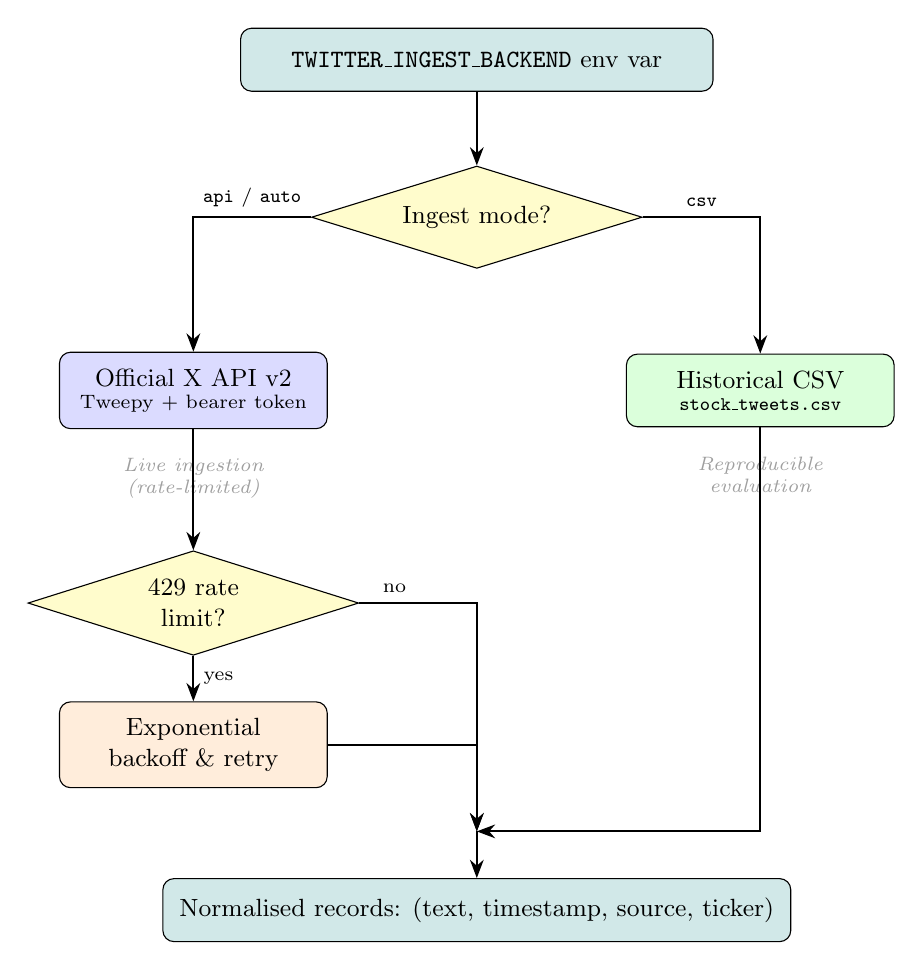
\begin{tikzpicture}[
  every node/.style={font=\small},
  dec/.style  ={draw, diamond, fill=yellow!20, aspect=2.6,
                minimum width=4.2cm, inner sep=3pt, align=center},
  back/.style ={draw, rounded corners=4pt, fill=#1,
                minimum width=3.4cm, minimum height=0.90cm,
                align=center, inner sep=6pt},
  io/.style   ={draw, rounded corners=4pt, fill=teal!18,
                minimum width=6.0cm, minimum height=0.80cm,
                align=center, inner sep=6pt},
  note/.style ={font=\scriptsize\itshape, text=gray!75, align=center},
  arr/.style  ={->, >=Stealth, thick}]

%% Top: env var selector
\node[io]  (env)     at ( 0,   0.0) {\texttt{TWITTER\_INGEST\_BACKEND} env var};
\node[dec] (mode)    at ( 0,  -2.0) {Ingest mode?};

%% Two nodes: live API vs historical CSV
\node[back=blue!14]   (api)  at (-3.6, -4.2) {Official X API v2\\[-3pt]\scriptsize Tweepy + bearer token};
\node[back=green!14]  (csv)  at ( 3.6, -4.2) {Historical CSV\\[-3pt]\scriptsize \texttt{stock\_tweets.csv}};

%% Notes below each branch
\node[note, below=0.25cm of api] {Live ingestion\\(rate-limited)};
\node[note, below=0.25cm of csv] {Reproducible\\evaluation};

%% Rate-limit handling on the API side
\node[dec] (ratelim)  at (-3.6, -6.9) {429 rate\\limit?};
\node[back=orange!14] (backoff) at (-3.6, -8.7) {Exponential\\backoff \& retry};

%% Output + merge hub (both paths converge here before persistence)
\node[io]  (out)      at ( 0,  -10.8) {Normalised records: (text, timestamp, source, ticker)};
\coordinate (merge) at (0,-9.8);

%% Arrows: env -> mode
\draw[arr] (env)  -- (mode);

%% mode -> api (L-shape: down from mode.west corner, then straight down to api)
\draw[arr] (mode.west) -|
    node[pos=0.25, above, font=\scriptsize]{\texttt{api} / \texttt{auto}}
    (api.north);

%% mode -> csv (L-shape on the right)
\draw[arr] (mode.east) -|
    node[pos=0.25, above, font=\scriptsize]{\texttt{csv}}
    (csv.north);

%% api -> ratelim (straight down, same x-coordinate)
\draw[arr] (api.south) -- (ratelim.north);

%% ratelim -> backoff ("yes" branch, straight down)
\draw[arr] (ratelim.south) -- node[right, font=\scriptsize]{yes} (backoff.north);

%% ratelim "no" branch -> merge (right then down)
\draw[arr] (ratelim.east) -|
    node[pos=0.15, above, font=\scriptsize]{no}
    (merge);

%% backoff -> merge (right then down)
\draw[arr] (backoff.east) -| (merge);

%% csv -> merge (down then left)
\draw[arr] (csv.south) |- (merge);

%% merge -> out (final arrow down to shared schema)
\draw[arr] (merge) -- (out.north);
\end{tikzpicture}
\caption{X/Twitter ingestion architecture. Live collection uses the official X API v2 via Tweepy with an exponential-backoff handler for 429 rate-limit responses. A historical CSV path provides a fixed, reproducible evaluation corpus. Both paths emit the same normalised record schema, keeping the downstream pipeline indifferent to which path was active.}
\label{fig:twitter_backend}
\end{figure}

Restricting Twitter collection to the official API was a deliberate decision. The X platform's terms of service prohibit unauthorised scraping of public posts, and relying exclusively on the documented interface keeps the pipeline aligned with those terms and with the project's Ethics Awareness Form commitments (Appendix~\ref{app:ethics}). The practical cost of that decision, however, is real. Free-tier rate and quota limits on the v2 endpoints were substantially tightened during the 2023--2024 platform changes, and the quota available within an undergraduate project budget does not support the tweet volumes reported in earlier academic studies that pre-date those changes. In early testing I reached the monthly cap well before obtaining a corpus comparable in size to the Reddit or NewsAPI feeds. This is the root cause of the Twitter subcorpus being the smallest of the three sources in this system. Where Twitter sentiment is surfaced in the dashboard I therefore treat it as a secondary, corroborating signal rather than as a primary input. The correlation engine's per-source filters make that imbalance explicit to users.

\subsection{News Ingestion}

Financial news is collected via the NewsAPI \texttt{/everything} endpoint (\texttt{ingest\_news.py}), targeting major outlets including Reuters and Bloomberg under business and finance category filters. A configurable keyword query (e.g., ``stock market OR earnings OR Fed rate'') is combined with source-level filtering. The NewsAPI client is authenticated via \texttt{NEWS\_API\_KEY}, and pagination is handled automatically. One problem I had not anticipated was the volume of syndicated duplicate content: the same Reuters or AP wire article would appear under dozens of different publisher names, meaning a naive ingest would count it as many separate data points. I addressed this with content-hash deduplication and URL-based deduplication at ingestion time. Artefacts introduced by NewsAPI's response format (e.g., ``[+\textit{N} chars]'' truncation indicators) are also stripped during cleaning.

\subsection{Supplementary Ingestion Pipelines}

Two additional ingest pipelines are maintained for bulk historical data collection:
\begin{itemize}
    \item \path{ingest_huggingface_financial_tweets.py}: streams the Hugging Face dataset \path{StephanAkkerman/financial-tweets-stocks} and recomputes sentiment using FinBERT.
    \item \path{ingest_felixdrinkall_yahoo_news.py}: ingests a 2017--2023 Yahoo Finance news archive, providing a multi-year historical baseline for correlation analysis.
\end{itemize}

\subsection{Automated Scheduling}

Continuous data collection is orchestrated through two GitHub Actions workflows.  The daily workflow (\texttt{collect-data.yml}) runs Reddit, NewsAPI, and X/Twitter ingestion in sequence, passes results through the FinBERT inference stack, and writes labelled records to the Neon PostgreSQL database.  A separate weekly workflow (\texttt{collect-reddit-bulk.yml}) performs a deeper Reddit pull across a broader ticker list.  Both workflows cache Hugging Face model weights using a hash of \texttt{requirements.txt} as the cache key, avoiding redundant downloads across runs.

\section{Preprocessing Pipeline}
\label{sec:preprocessing}

The preprocessing module (\texttt{app/pipelines/preprocess\_data.py}) implements four named configuration profiles, selected at runtime via a \texttt{--config} argument.  The \texttt{finbert} profile, used exclusively for sentiment inference, is designed to preserve the contextual integrity required by the transformer architecture:

\noindent
\begin{minipage}{\linewidth}
\begin{lstlisting}[language=Python, caption={FinBERT preprocessing configuration in \texttt{preprocess\_data.py}.}, label={lst:finbert_config}]
CONFIGS = {
    "finbert": {
        "lowercase": False,           # Preserve case (tickers, proper nouns)
        "remove_urls": True,
        "remove_stopwords": False,    # Full context required for attention
        "lemmatize": False,           # Subword tokenisation handles variants
        "preserve_financial": True,
        "preserve_financial_punctuation": True,  # Retain %, $, decimals
        "handle_negations": True,     # "not profitable" -> "not_profitable"
    }
}
\end{lstlisting}
\end{minipage}

All processed records are stored with both the original and cleaned text, along with a \path{text_cleaned} field and source-specific metadata.  Source-text field mapping (\path{SOURCE_TEXT_FIELDS}) ensures that the correct JSON key is extracted for each platform (e.g., Reddit's \path{title} plus \path{selftext}, Twitter's \path{text}, NewsAPI's \path{clean_title} plus \path{clean_description}).

\section{Sentiment Inference Engine}
\label{sec:inference_engine}

The FinBERT model is encapsulated in the \texttt{FinBERTModel} class within \path{app/models/finbert_model.py}, loaded from the \path{ProsusAI/finbert} checkpoint via Hugging Face Transformers.  A singleton accessor \texttt{get\_model()} ensures the model is loaded once per process, avoiding repeated initialisation overhead.  Inference is performed with a configurable batch size (default 32) and a maximum sequence length of 512 tokens.

The \texttt{analyze\_batch()} function in \texttt{app/models/sentiment\_inference.py} provides the production batch interface and returns a tuple of results and a \texttt{FailedItemsTracker} instance:

\noindent
\begin{minipage}{\linewidth}
\begin{lstlisting}[language=Python, caption={Production batch inference signature in \texttt{sentiment\_inference.py}.}, label={lst:batch_inference}]
def analyze_batch(
    texts: List[str],
    batch_size: int = 32,
    return_all_scores: bool = False,
    skip_errors: bool = True,
    track_failures: bool = True,
) -> tuple[List[Optional[Dict]], Optional[FailedItemsTracker]]:
    """
    Analyse sentiment for multiple texts.

    Returns a (results, tracker) tuple.  Each result is a dict:
        {"label": "positive"|"negative"|"neutral",
         "score": float,
         "scores": {"positive": ..., "negative": ..., "neutral": ...}}
    Failed items are logged in the tracker rather than raising.
    """
\end{lstlisting}
\end{minipage}

Empty texts are filtered before the model call and tracked in the \texttt{FailedItemsTracker}, preserving original index alignment in the returned list.

The FinBERT tokeniser module (\texttt{app/preprocessing/finbert\_tokenizer.py}) provides standalone tokenisation with padding, truncation, and attention mask generation, decoupled from the model class so unit tests can call tokenisation alone.

\section{Novel: Finance-Emotion Taxonomy}
\label{sec:emotion_impl}

The finance-emotion module (\path{app/analysis/finance_emotion.py}) implements the taxonomy described in Section~\ref{sec:emotion_design}.  Six emotion categories are defined with curated domain lexicons:

\begin{itemize}
    \item \textbf{fear}: ``selloff'', ``panic'', ``crash'', ``plunge'', ``bankruptcy'', ``tariff'', ``bearish'', etc.
    \item \textbf{optimism}: ``beat'', ``surge'', ``rally'', ``bullish'', ``momentum'', ``breakout'', etc.
    \item \textbf{uncertainty}: ``uncertain'', ``volatility'', ``mixed'', ``guidance cut'', ``headwind'', etc.
    \item \textbf{confidence}: ``conviction'', ``resilient'', ``outperform'', ``strong balance sheet'', ``moat'', etc.
    \item \textbf{scepticism}: ``overvalued'', ``hype'', ``bubble'', ``priced for perfection'', etc.
    \item \textbf{mixed}: assigned when no single emotion achieves sufficient confidence.
\end{itemize}

The inference function \texttt{infer\_finance\_emotion()} accepts the FinBERT softmax vector, normalised Shannon entropy, and extracted aspect snippets as inputs.  It initialises base scores, applies probability-weighted increments, adds lexicon hit scores, and adds aspect-specific priors before normalising to a probability simplex.  A dominant emotion is selected only if its score exceeds a minimum threshold and is sufficiently differentiated from the second-ranked emotion; otherwise, \textit{mixed} is returned.  The output dictionary includes the dominant label, its score, the full distribution, and a human-readable rationale string for display in the dashboard.

\section{Novel: Aspect-Based Sentiment Analysis (ABSA-Lite)}
\label{sec:absa_impl}

The financial sentiment enrichment module (\path{app/analysis/financial_sentiment_enrichment.py}) implements the lightweight ABSA described in Section~\ref{sec:absa_design}.  The \texttt{extract\_aspect\_snippets()} function segments documents into sentences using a regex-based splitter and matches each sentence against the six aspect keyword buckets.  Up to eight evidence snippets are returned per document (maximum two per aspect) with their aspect tag and optional FinBERT per-snippet label.

A \texttt{normalized\_label\_entropy()} function computes $H_{\text{norm}} = -\sum_i p_i \log p_i / \log 3$ over the FinBERT softmax distribution, producing a score in $[0, 1]$ where 0 indicates a decisive one-class prediction and 1 indicates maximum distributional uncertainty.  This entropy value feeds directly into the emotion inference pipeline and is exposed in the API response as an uncertainty indicator.

\section{Stock Entity Resolution}
\label{sec:entity_impl}

The entity resolution subsystem spans three files: \path{app/entities/stock_database.py} (ticker and company-name lookup), \path{app/entities/company_extractor.py} (spaCy NER candidate extraction), and \path{app/entities/entity_resolver.py} (the three-stage string-matching cascade). The two-component structure is deliberate: the heavyweight spaCy pipeline runs once per document in \texttt{CompanyExtractor} to produce candidate spans, and the \texttt{EntityResolver} then operates purely on strings, which makes the resolution logic independently unit-testable and allows either component to be substituted in future iterations.

The \texttt{EntityResolver.resolve()} method implements a three-stage priority cascade over its candidate input: (1)~exact cashtag match (\texttt{\$AAPL} → \texttt{AAPL}); (2)~exact company-name match against the canonical name index; (3)~fuzzy partial-ratio match using FuzzyWuzzy with a configurable similarity threshold (default 0.85). A blacklist of 12 common false-positive entities (``Fed'', ``SEC'', ``FBI'', ``White House'', etc.) is applied inside the resolver to prevent systematic misclassification of regulatory and government body mentions.

\section{XAI: LIME Integration}
\label{sec:xai_impl}

\subsection{LIME Explainer}

The \texttt{LIMEExplainer} class is implemented in \path{app/explainability/lime_explainer.py}.  It wraps a \texttt{LimeTextExplainer} singleton with a probability adapter that maps any free-text input to FinBERT's three-class probability distribution.  The adapter normalises inputs, tokenises using FinBERT's WordPiece tokeniser, runs inference, and returns a matrix of shape $N \times 3$.  This black-box interface decouples the explainer from FinBERT's internals, permitting future model substitution without modifying the explanation logic.

\noindent
\begin{minipage}{\linewidth}
\begin{lstlisting}[language=Python, caption={LIME \texttt{/explain} handler (excerpt from \texttt{sentiment.py}).}, label={lst:lime_endpoint}]
@router.post("/explain", response_model=ExplainResponse)
async def explain(body: ExplainRequest):
    """Generate token-level LIME explanation for a single text."""
    # Run CPU-heavy LIME in the default thread-pool executor to avoid
    # blocking the FastAPI event loop. ``asyncio.to_thread`` is the
    # Python 3.9+ high-level wrapper over ``loop.run_in_executor(None, ...)``.
    explanation = await asyncio.to_thread(
        run_lime_explain, body.text, body.options
    )
    tokens = [
        ExplanationToken(token=t, weight=w)
        for t, w in explanation["top_features"]
    ]
    return ExplainResponse(
        text=body.text,
        prediction=SentimentResult(**explanation["prediction"]),
        tokens=tokens,
        metadata={"method": "LIME", "processing_time_ms": explanation["time_ms"]},
    )
\end{lstlisting}
\end{minipage}

The \texttt{asyncio.to\_thread} pattern is architecturally important: LIME perturbation sampling is a CPU-bound computation that can take several seconds per explanation. \texttt{asyncio.to\_thread} is a thin Python~3.9+ wrapper over \texttt{loop.run\_in\_executor(None, ...)}, so the computation is dispatched to the event loop's default thread-pool executor without a call to \texttt{get\_event\_loop()}. This prevents the FastAPI server from blocking other concurrent requests during explanation generation.  The frontend allocates a 120-second timeout budget to this endpoint to accommodate inference on complex, long-form posts.

\subsection{SHAP Explainer}

The \texttt{SHAPExplainer} class (\path{app/explainability/shap_explainer.py}) provides token-level Shapley value attribution using the \texttt{shap.Explainer} with the FinBERT tokeniser as the masker.  SHAP values are computed per token per class, and the \texttt{get\_summary\_data()} method aggregates token importance across a corpus, excluding special tokens (\texttt{[CLS]}, \texttt{[SEP]}, \texttt{[PAD]}).  SHAP is available via the API's \path{/api/v1/explainability/shap} route (served from the \path{backend/api/} router) and through the Jupyter notebook \path{notebooks/06-shap-explainability.ipynb}, but is not rendered in the production frontend due to latency constraints.  Ten pre-generated LIME explanation artefacts (PNG bar charts and HTML files) are stored in \texttt{data/processed/explanations/lime\_examples/} and are referenced in the evaluation chapter.

\section{REST API}
\label{sec:api_impl}

\subsection{Application Structure}

The canonical FastAPI application is defined in \path{backend/app/main.py}.  It registers three middleware layers (in innermost-to-outermost order): \texttt{SecurityHeadersMiddleware} (sets HTTP security headers), \texttt{APIKeyMiddleware} (enforces the \texttt{API\_KEY} environment variable on protected routes in production), and \texttt{CORSMiddleware} (permitting cross-origin requests from the React dev server).  A \texttt{TrustedHostMiddleware} is conditionally registered when the \texttt{ALLOWED\_HOSTS} environment variable is set.

The versioned API router is assembled in \path{app/api/v1/router.py} and includes the following sub-routers:

\begin{table}[ht]
  \centering
  \footnotesize
  \setlength{\tabcolsep}{3pt}
  \caption{Primary REST API endpoints exposed by \texttt{backend/app/main.py}.}
  \label{tab:api-routes}
  \begin{tabular}{@{}>{\raggedright\arraybackslash}p{0.24\linewidth}>{\raggedright\arraybackslash}p{0.30\linewidth}>{\raggedright\arraybackslash}p{0.40\linewidth}@{}}
    \toprule
    \textbf{Prefix} & \textbf{Key Endpoints} & \textbf{Description} \\
    \midrule
    \path{/api/v1/sentiment} & \makecell[tl]{\path{/analyze}\\\path{/batch}\\\path{/explain}\\\path{/narrative}} & FinBERT inference, batch analysis, LIME explanation, Groq-backed ticker narrative \\
    \path{/api/v1/data} & \makecell[tl]{\path{/predictions}\\\path{/statistics}\\\path{/stock-quality/}\texttt{\{t\}}} & Historical records, global statistics, per-ticker data quality \\
    \path{/api/v1/correlation} & \makecell[tl]{\texttt{\{ticker\}}\\\path{/timeseries}\\\path{/lag-analysis}\\\path{/granger}\\\path{/rolling}} & Sentiment-price statistics with configurable methodology \\
    \path{/api/v1/stocks} & \makecell[tl]{\path{/analyze}\\\texttt{/\{t\}/sentiment}\\\path{/trending}\\\path{/compare}} & Entity-resolved per-ticker analytics \\
    \bottomrule
  \end{tabular}
\end{table}

In lean deployment mode (\path{LEAN_API=1}), the \path{/sentiment} prefix is routed to \path{app/api/v1/sentiment_lean.py}, which returns \texttt{503 Service Unavailable} with a descriptive message for \path{/analyze}, \path{/batch}, and \path{/explain}, while \path{/narrative} (Groq-backed, no PyTorch dependency) remains operational.

\subsection{Health Endpoints}

Two health endpoints are provided for deployment monitoring:
\begin{itemize}
    \item \texttt{GET /health}: liveness probe; returns \texttt{\{"status": "ok"\}} immediately without dependency checks.
    \item \texttt{GET /health/ready}: readiness probe; executes a \texttt{SELECT 1} against the database; returns 503 if the database is unreachable.
\end{itemize}

This split follows the Kubernetes liveness/readiness pattern and ensures that load balancers can distinguish between a process that is alive but waiting for the database (readiness failure) versus one that has crashed (liveness failure).

\section{Correlation Analysis Implementation}
\label{sec:correlation_impl}

The \texttt{CorrelationAnalyzer} class (\path{app/analysis/correlation.py}) performs all statistical computations and is initialised once per process via \texttt{lru\_cache}.  Results are cached using a TTL-backed \texttt{cachetools.TTLCache} with a one-hour expiry and 256-entry capacity, preventing repeated computation of expensive Granger and OLS calculations for popular tickers.

For Granger causality, the implementation first checks for \texttt{statsmodels} availability at import time and degrades gracefully to a no-test result if the package is absent.  When available, the augmented Dickey-Fuller test is applied to both series to verify stationarity before running the Granger F-test at configurable lag orders.  Market adjustment via SPY beta residualisation ($y_\text{adj} = y - \hat{\beta} \cdot x_\text{SPY}$) is optionally applied to the return series before correlation computation, isolating asset-specific sentiment signals from broad market co-movement.

\section{React Frontend}
\label{sec:frontend_impl}

The React~18 single-page application is built with Vite~5 and TypeScript.  All chart components use \textbf{Recharts}, which provides a composable, SVG-based charting library well-suited for responsive financial time-series visualisation.  State management is handled via React hooks (\texttt{useState}, \texttt{useEffect}, \texttt{useMemo}), with all API calls centralised in \texttt{src/services/api.ts} using Axios.

The \textbf{Market Overview} page (\texttt{MarketOverview.tsx}) renders a global sentiment distribution pie chart, a daily trend bar chart, and a per-source comparison using data from \texttt{/api/v1/data/statistics}.  Source filter controls (\textit{All}, \textit{Reddit}, \textit{News}, \textit{X}) and a date-range selector update all charts simultaneously via a shared filter state.

The \textbf{Stock Analysis} page (\texttt{StockAnalysis.tsx}) provides per-ticker analytics: a sentiment time-series with price overlay sourced from the correlation timeseries route (\path{/api/v1/correlation/<ticker>/timeseries}, with \texttt{<ticker>} replaced by the selected symbol at runtime), a finance-emotion breakdown, LIME explanation heatmap (tokens coloured by weight), and a data quality indicator panel.  A dedicated narrative card calls \path{/api/v1/sentiment/narrative} to retrieve a Groq-generated LLM summary of recent ticker sentiment, grounded in database records.

\subsection{Dashboard Screenshots}
\label{sec:frontend_screenshots}

Figures~\ref{fig:screen_market_overview_a} to \ref{fig:screen_lime} show three principal views of the running dashboard.

\begin{figure}[p]
  \centering
  \IfFileExists{figures/screen_market_overview_1.png}{%
    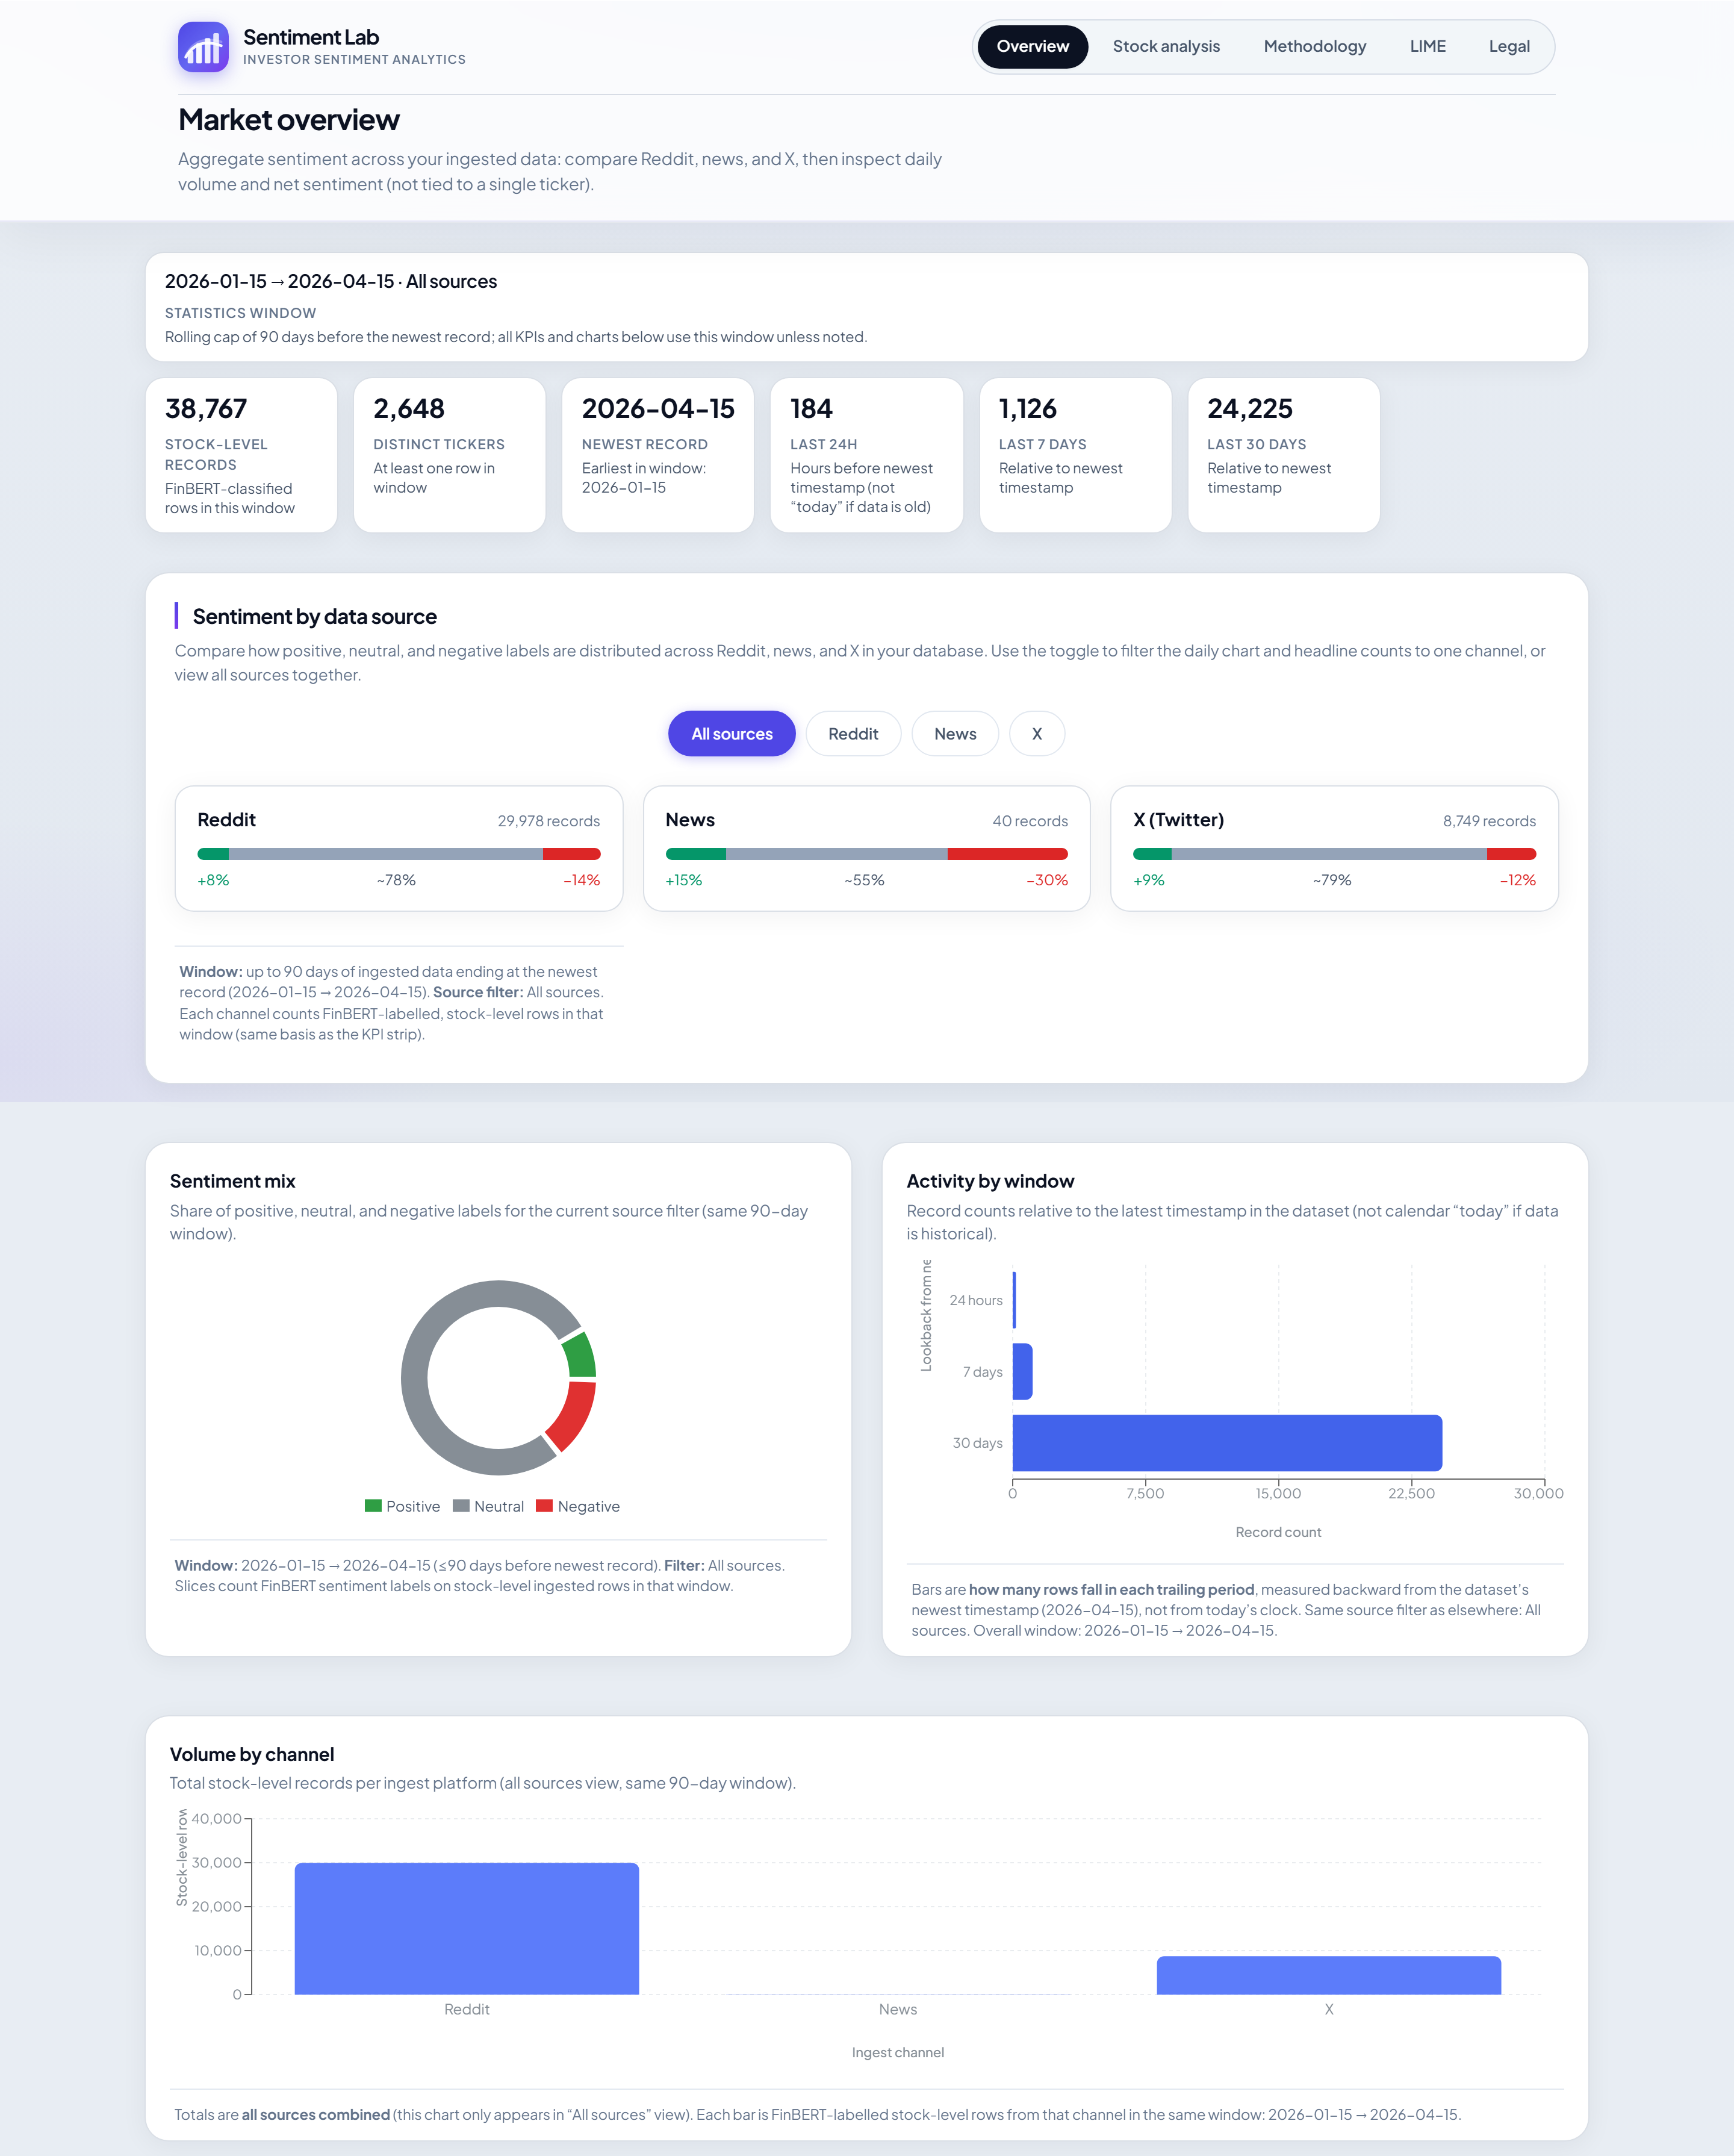
\includegraphics[width=\linewidth,height=0.82\textheight,keepaspectratio]{screen_market_overview_1.png}}{%
    \fbox{\parbox{0.88\linewidth}{\centering\vspace{2em}\texttt{screen\_market\_overview\_1.png} not found\vspace{2em}}}}
  \caption{Market Overview page (1 of 2): header, source filters, and global sentiment distribution.}
  \label{fig:screen_market_overview_a}
\end{figure}

\begin{figure}[p]
  \centering
  \IfFileExists{figures/screen_market_overview_2.png}{%
    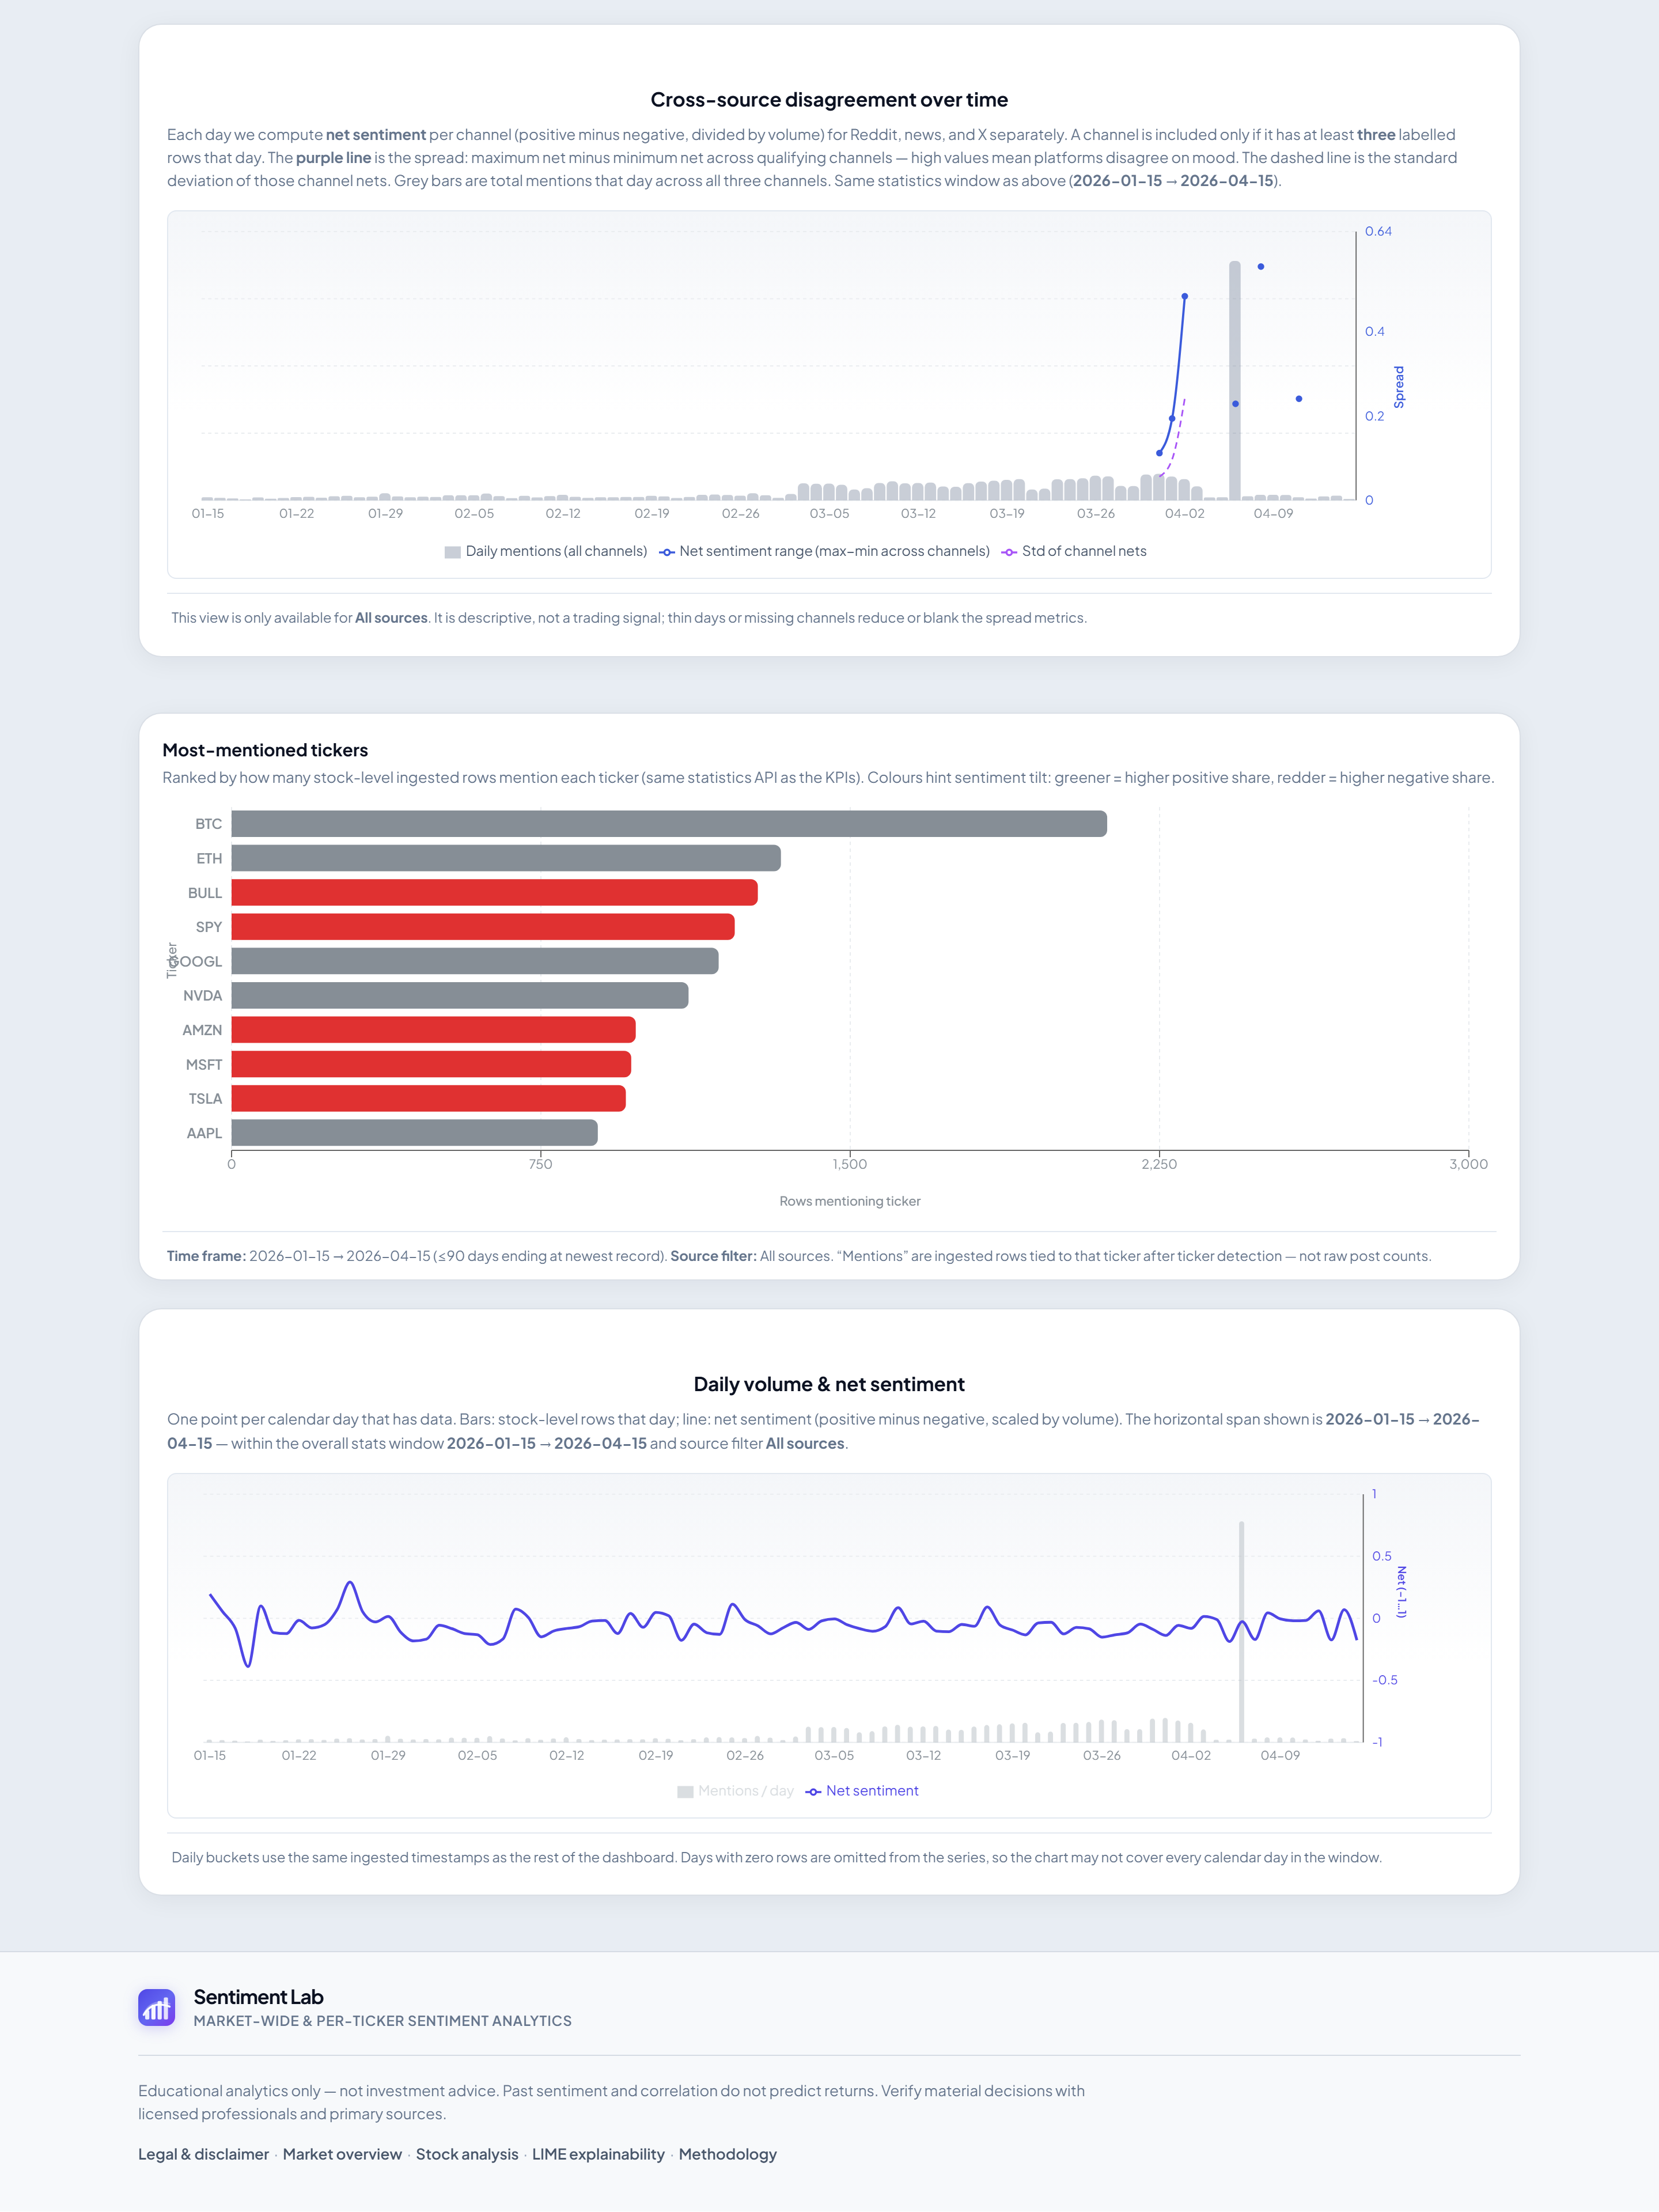
\includegraphics[width=\linewidth,height=0.82\textheight,keepaspectratio]{screen_market_overview_2.png}}{%
    \fbox{\parbox{0.88\linewidth}{\centering\vspace{2em}\texttt{screen\_market\_overview\_2.png} not found\vspace{2em}}}}
  \caption{Market Overview page (2 of 2): daily sentiment trend and top trending tickers.}
  \label{fig:screen_market_overview_b}
\end{figure}

\begin{figure}[p]
  \centering
  \IfFileExists{figures/screen_stock_analysis_1.png}{%
    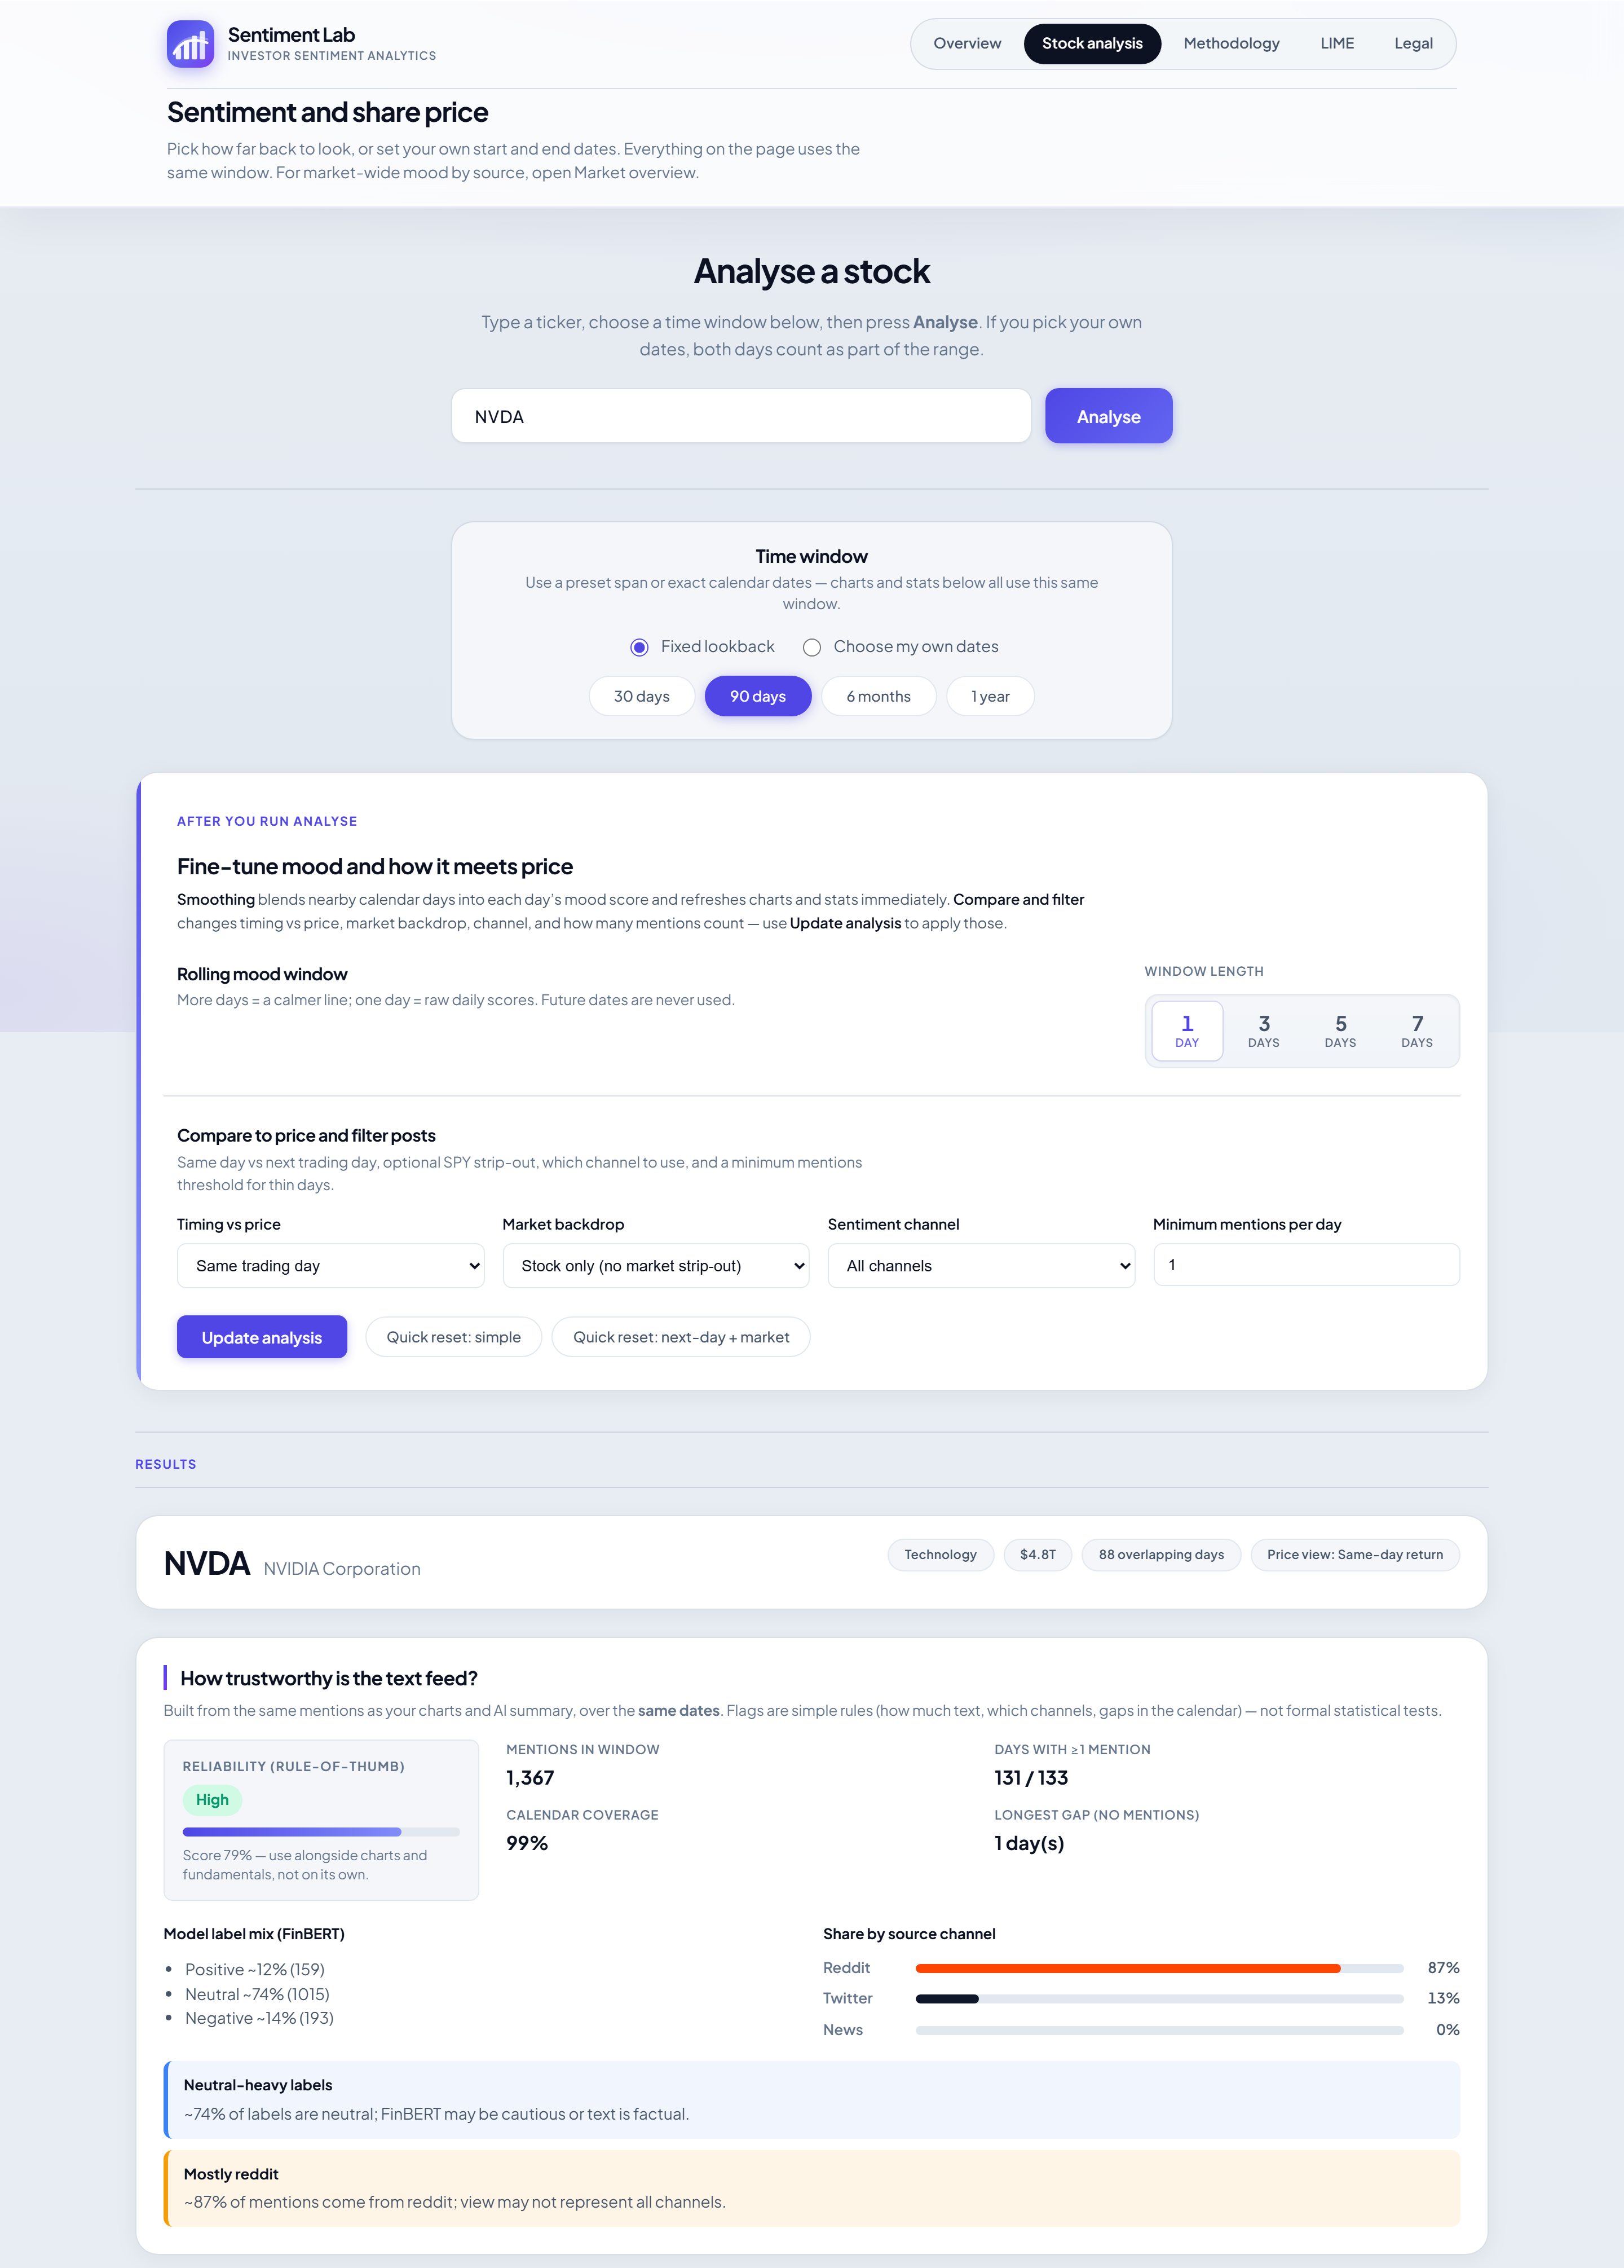
\includegraphics[width=\linewidth,height=0.82\textheight,keepaspectratio]{screen_stock_analysis_1.png}}{%
    \fbox{\parbox{0.88\linewidth}{\centering\vspace{2em}\texttt{screen\_stock\_analysis\_1.png} not found\vspace{2em}}}}
  \caption{Stock Analysis page (1 of 3): ticker selector, sentiment time-series, and price overlay.}
  \label{fig:screen_stock_analysis_a}
\end{figure}

\begin{figure}[p]
  \centering
  \IfFileExists{figures/screen_stock_analysis_2.png}{%
    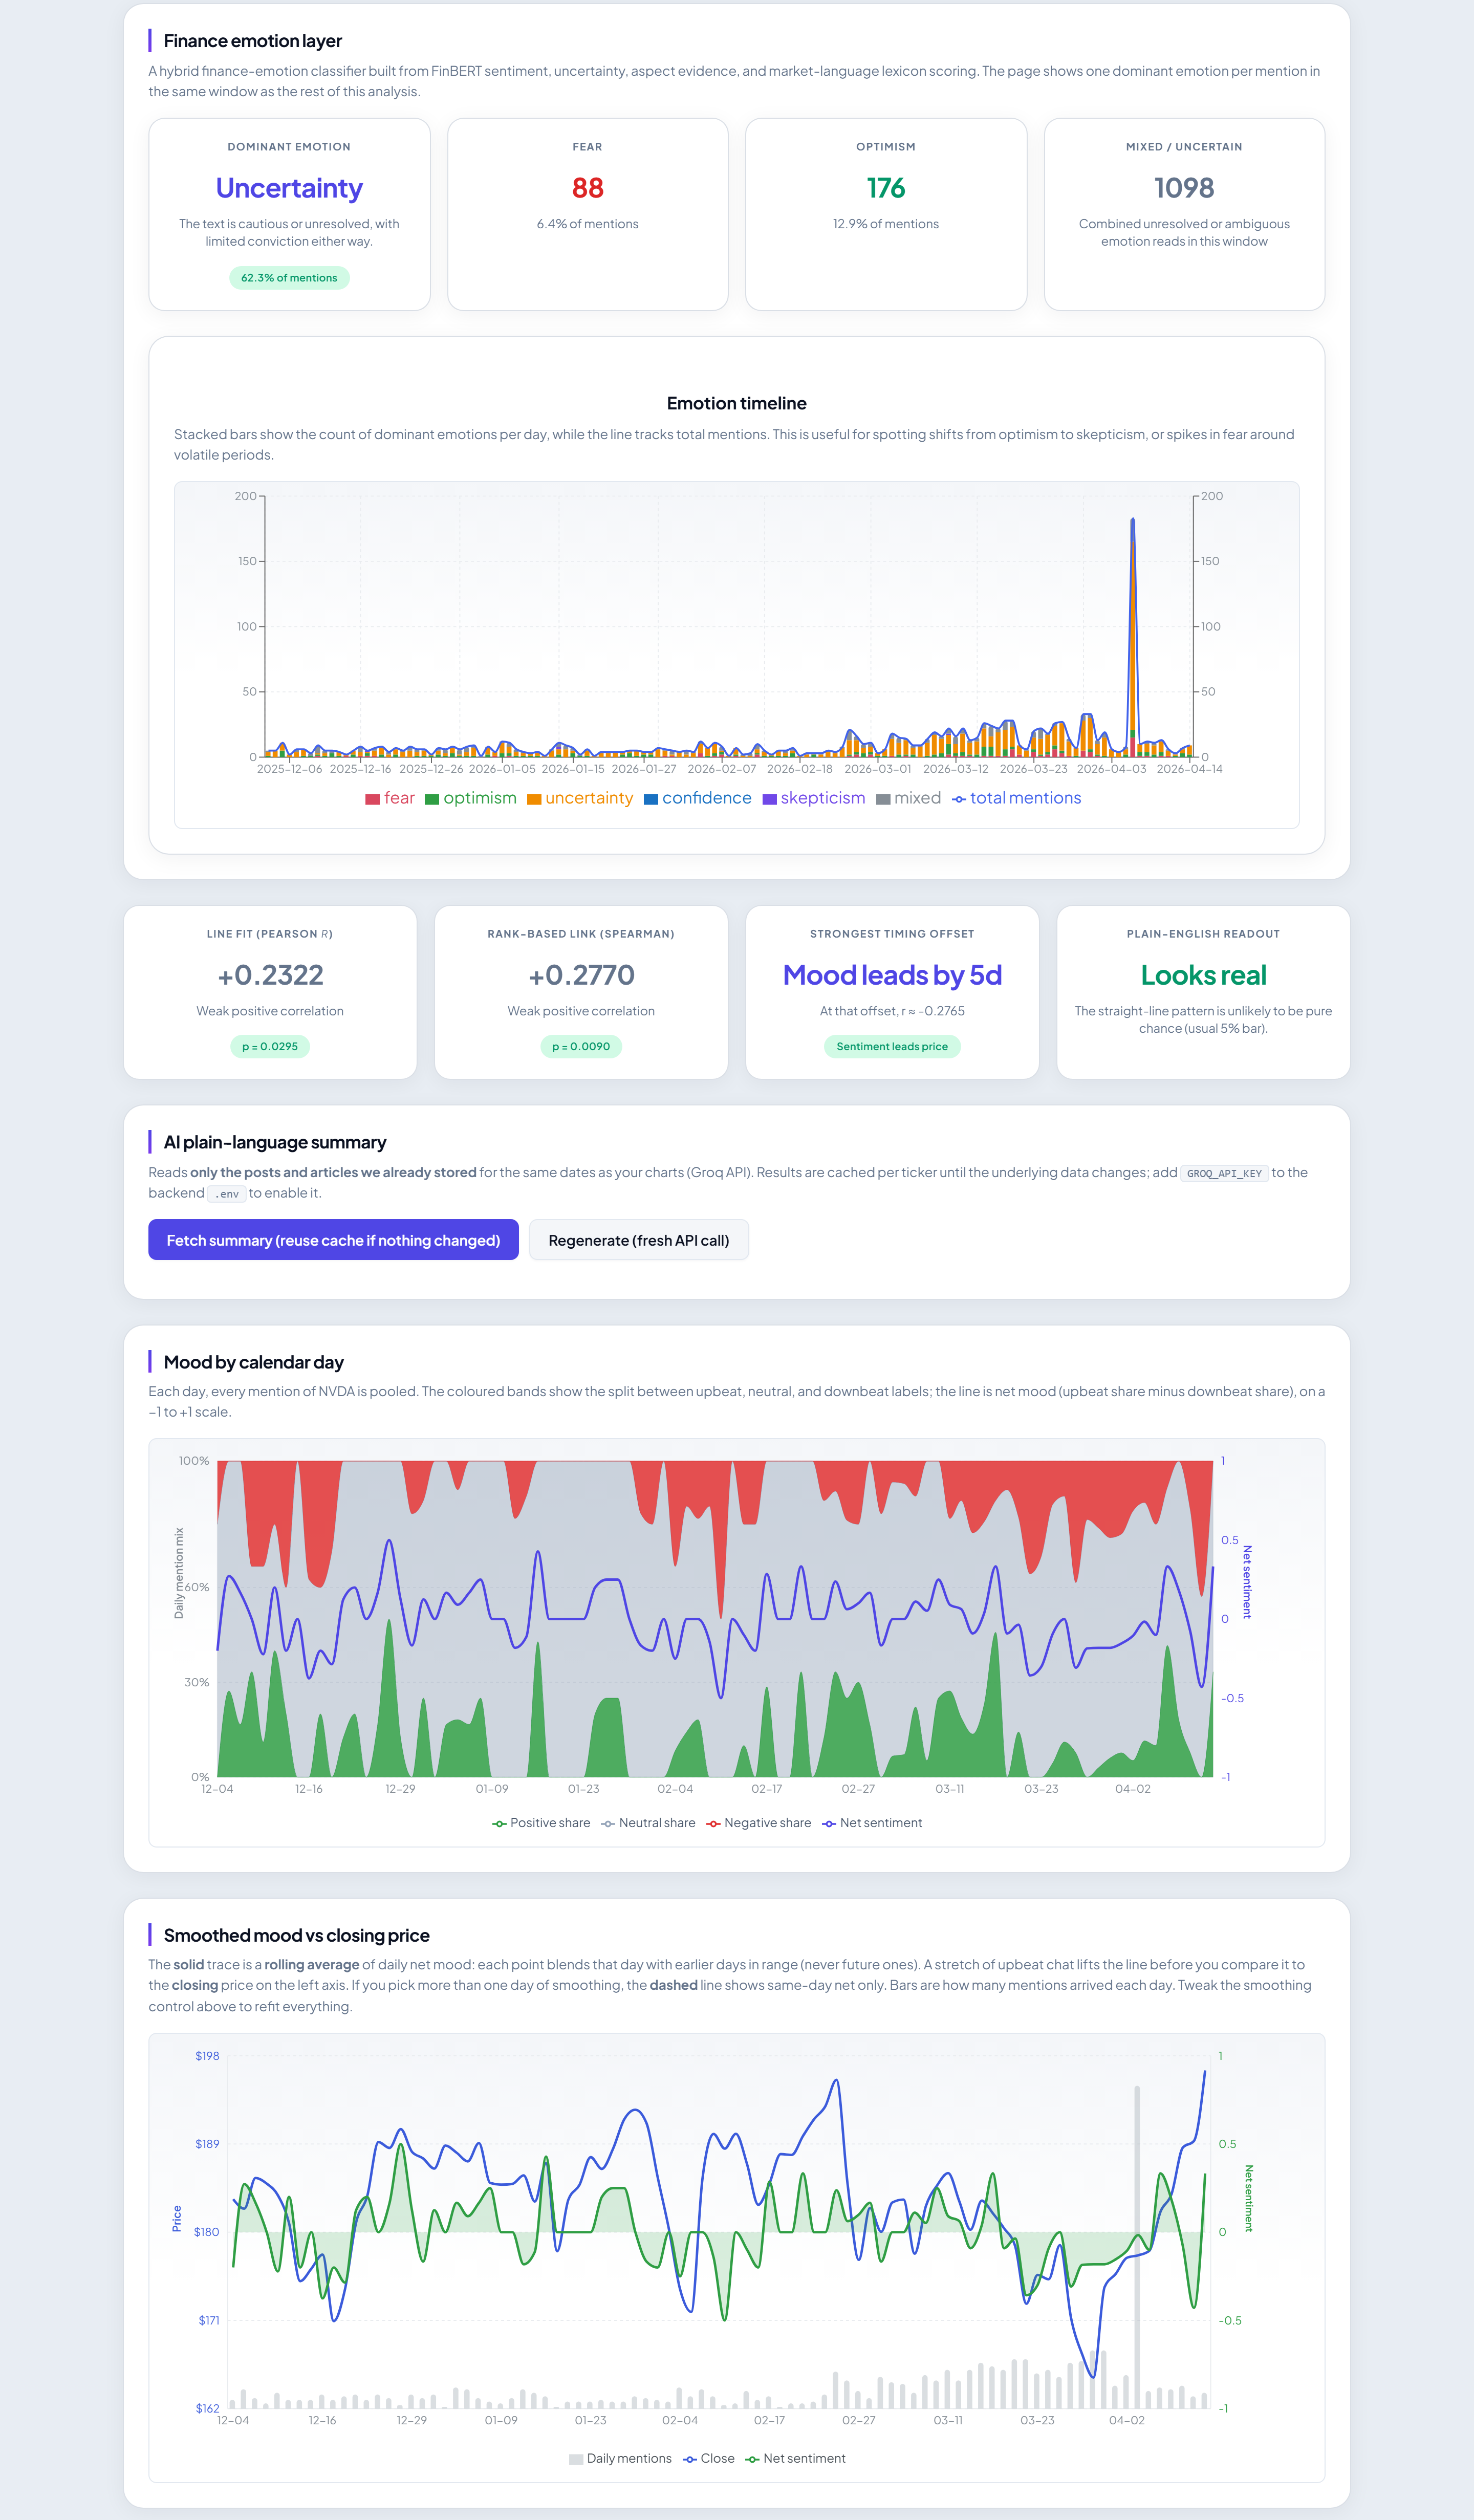
\includegraphics[width=\linewidth,height=0.82\textheight,keepaspectratio]{screen_stock_analysis_2.png}}{%
    \fbox{\parbox{0.88\linewidth}{\centering\vspace{2em}\texttt{screen\_stock\_analysis\_2.png} not found\vspace{2em}}}}
  \caption{Stock Analysis page (2 of 3): finance-emotion breakdown and per-source sentiment comparison.}
  \label{fig:screen_stock_analysis_b}
\end{figure}

\begin{figure}[p]
  \centering
  \IfFileExists{figures/screen_stock_analysis_3.png}{%
    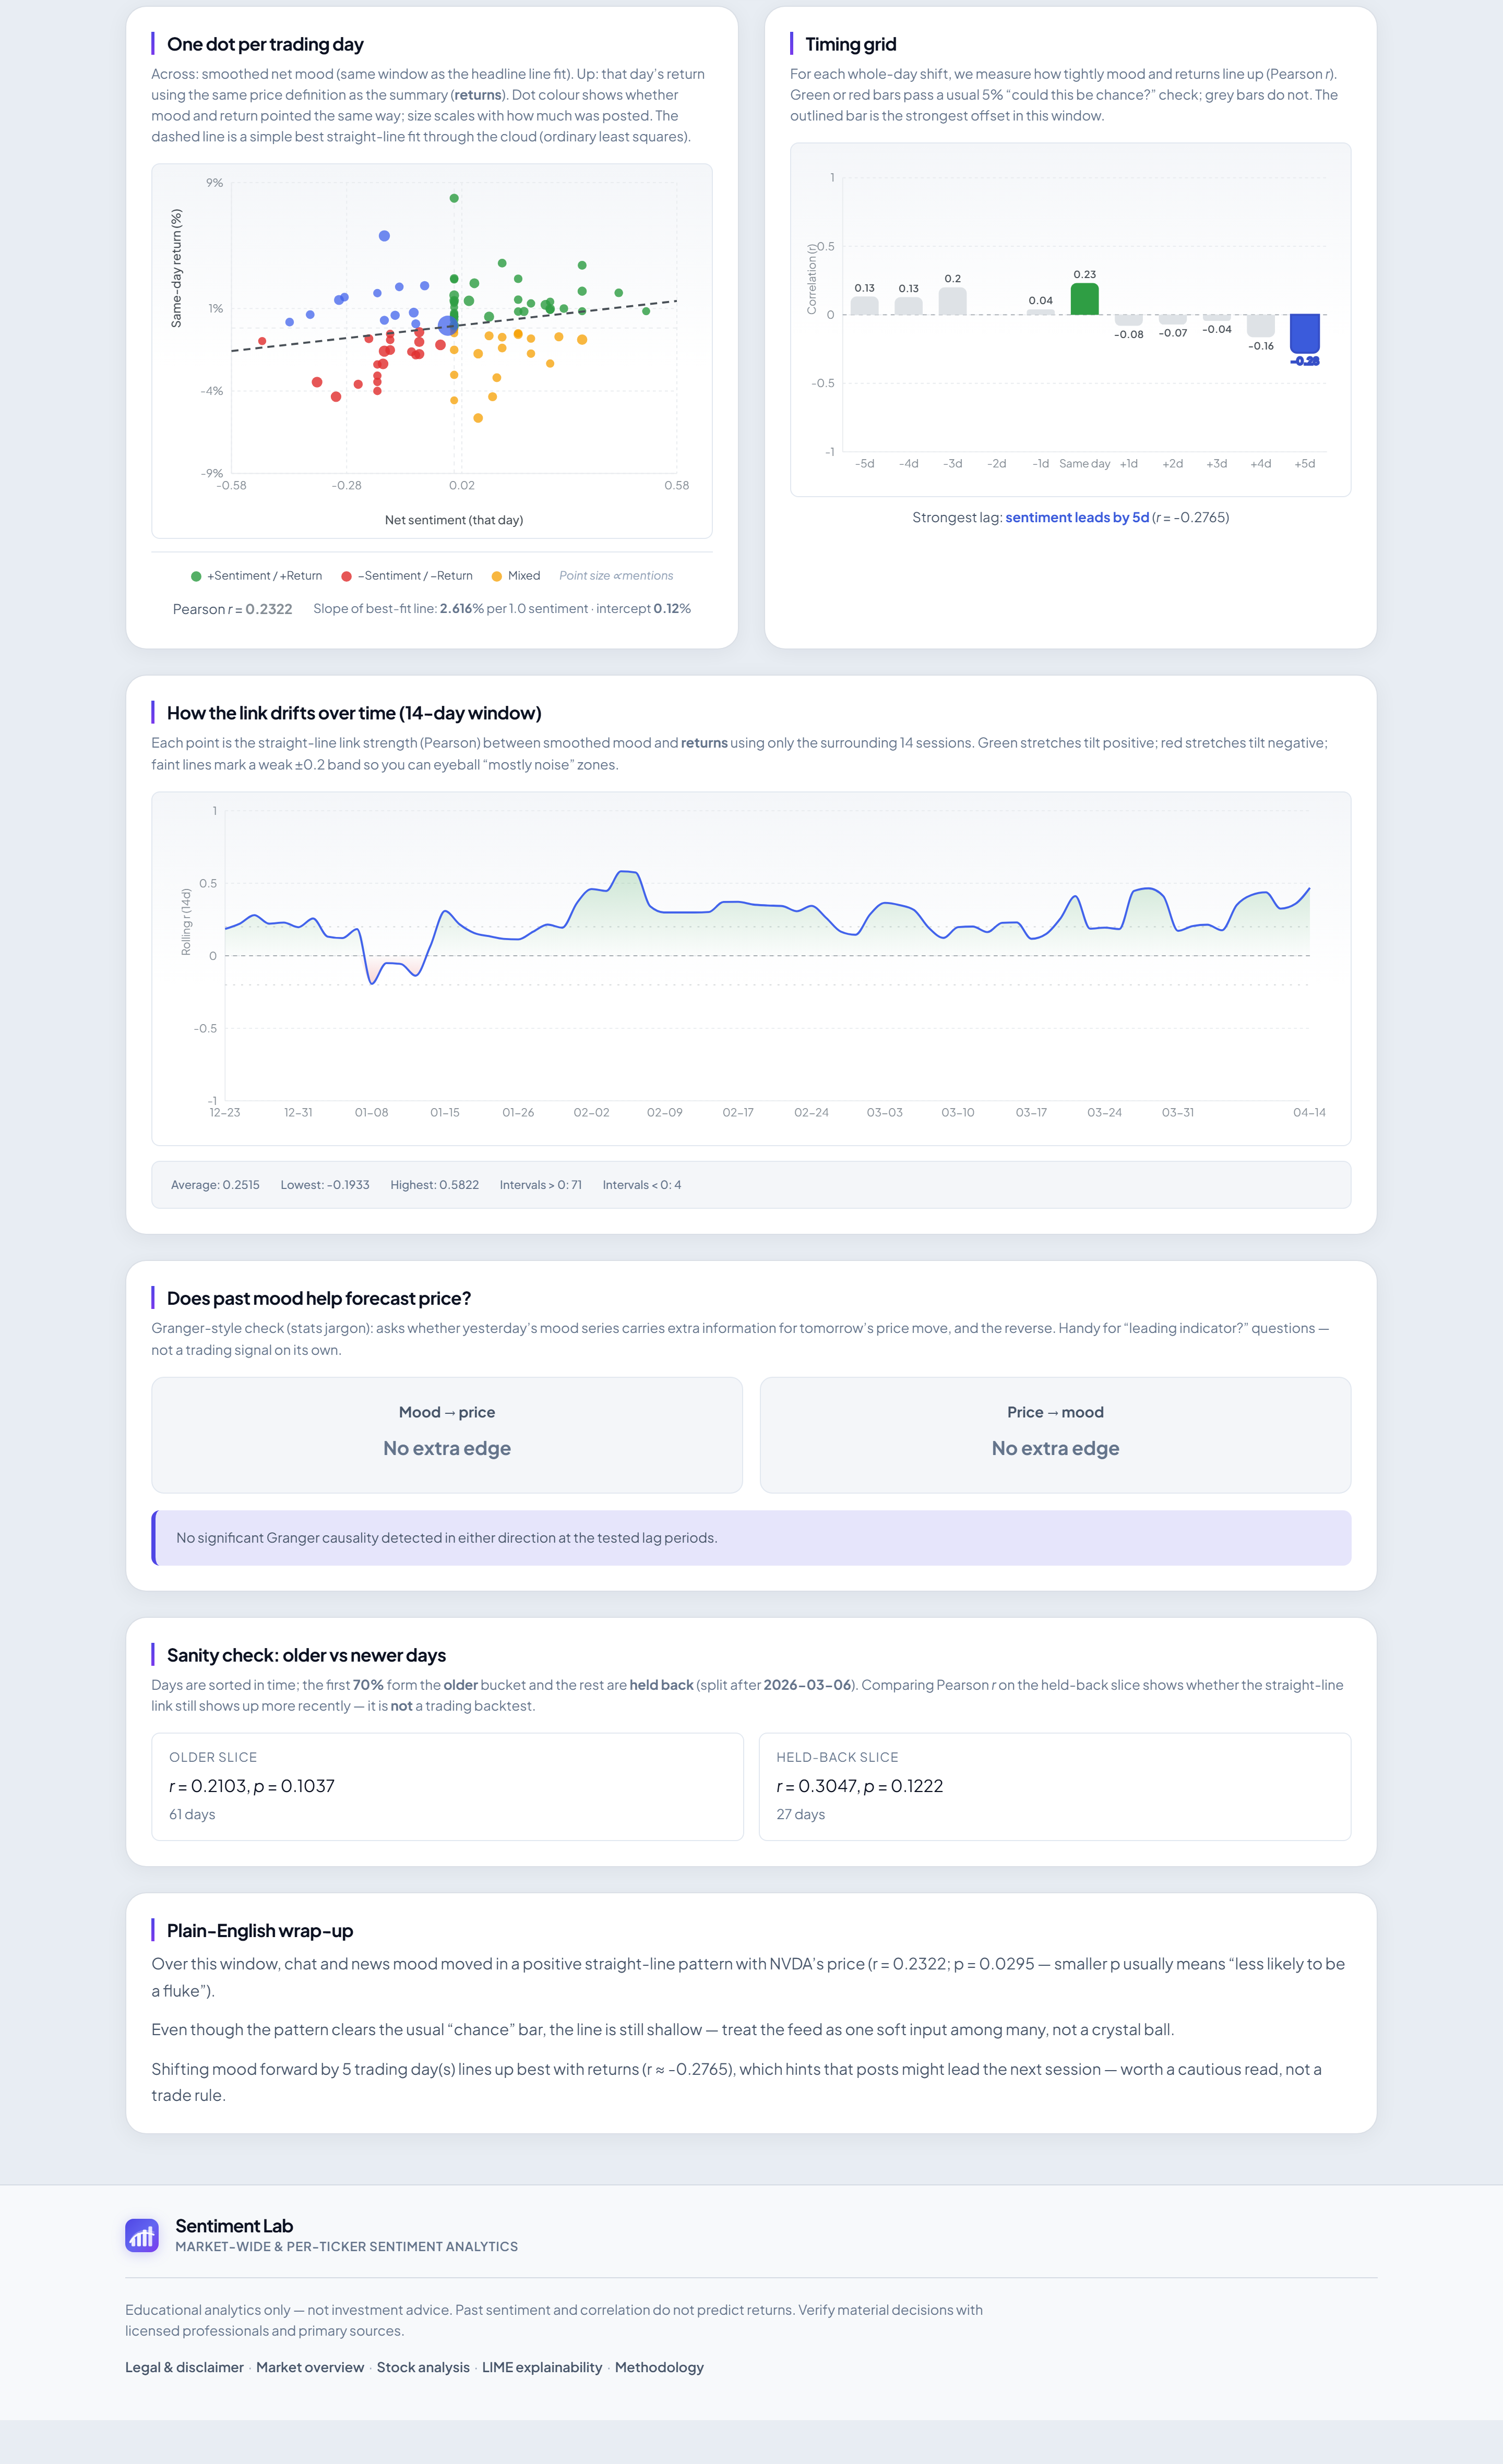
\includegraphics[width=\linewidth,height=0.82\textheight,keepaspectratio]{screen_stock_analysis_3.png}}{%
    \fbox{\parbox{0.88\linewidth}{\centering\vspace{2em}\texttt{screen\_stock\_analysis\_3.png} not found\vspace{2em}}}}
  \caption{Stock Analysis page (3 of 3): LIME token heatmap and data quality indicators.}
  \label{fig:screen_stock_analysis_c}
\end{figure}

\begin{figure}[p]
  \centering
  \IfFileExists{figures/screen_lime.png}{%
    \includeDashboardShot{screen_lime.png}}{%
    \fbox{\parbox{0.88\linewidth}{\centering\vspace{2.5em}LIME heatmap (\texttt{screen\_lime.png} not found)\vspace{2.5em}}}}
  \caption{LIME token heatmap rendered in the live dashboard, linking the explainability evaluation of Chapter~\ref{chap:evaluation} to the deployed user interface.}
  \label{fig:screen_lime}
\end{figure}

\section{Implementation Challenges and Resolutions}
\label{sec:challenges}

No part of this project went smoothly from the start. This section describes the most significant problems I encountered and how I resolved them.

\paragraph{Getting FinBERT to work at all.}
My initial experience with FinBERT was not straightforward. The first time I ran it, the process crashed on my development machine because I had not anticipated the memory requirements. Over the course of a few days I worked through three separate issues: getting the Hugging Face \texttt{transformers} library \citep{wolf2020transformers} model to load and cache correctly, reducing the batch size from larger values down to 32 to stay within the 8~GB VRAM budget of my consumer GPU, and confirming that attention masking was being applied correctly. I confirmed GPU utilisation using \texttt{torch.cuda.memory\_allocated()} profiling, which gave me visibility into memory consumption per batch. Once these were resolved the model was fast and stable. The initial setup, however, took far longer than I had expected.

\paragraph{Noticing the neutral recall problem.}
Before I ran any formal benchmarks, I was manually checking predictions on a sample of posts and noticed something odd. Text like ``The Federal Reserve held rates steady, in line with expectations'' was being labelled positive or negative rather than neutral. At first I thought I had a preprocessing bug. After investigating, I realised it was a characteristic of FinBERT's pre-training distribution, which is heavily skewed toward polarised financial language. The formal benchmark later confirmed this: FinBERT's neutral recall was 53.3\% while its precision was 97.0\%. In other words, the model was very conservative about labelling anything as neutral. I partially addressed this through the entropy score in the emotion taxonomy, which flags high-uncertainty predictions to the user rather than forcing a definitive label.

\paragraph{LIME latency in an async context.}
When I first tested LIME via the API, every request to the explanation endpoint blocked the entire server for the duration of the computation. LIME's perturbation sampling is CPU-bound and takes 15 to 40~seconds for a typical financial text. In a synchronous setup this would freeze all concurrent requests. I researched the correct pattern for offloading blocking work in FastAPI and found the \texttt{run\_in\_executor} approach. This hands the computation off to Python's thread pool while the event loop remains free to handle other requests. The pattern was not covered in my undergraduate modules, and implementing it correctly required independent reading of the asyncio documentation.

\paragraph{Memory management at batch scale.}
Processing large Reddit thread corpora occasionally produced out-of-memory errors even after the initial batch-size fix. I traced this to accumulated GPU memory not being released between batches. Adding explicit \texttt{torch.cuda.empty\_cache()} calls between batches resolved the issue, and I confirmed stable memory consumption with monitoring across several bulk ingestion runs.

\paragraph{Lean deployment on constrained cloud instances.}
Loading PyTorch and Transformers requires approximately 1.5~GB of RAM beyond the base Python process, which exceeds the free tier of several cloud hosting providers I evaluated. This is a concrete instance of the hidden dependency debt that Sculley et al.\ \citep{sculley2015debt} identify as one of the most common sources of maintenance cost in production ML systems. Rather than pay for a larger instance just to run FinBERT, I built the lean deployment mode. The \texttt{LEAN\_API} flag routes the \texttt{/sentiment} prefix to a stub module that returns \texttt{503 Service Unavailable} for inference-heavy endpoints, while all database and correlation endpoints remain operational. This means the analytical side of the dashboard stays usable even when the ML components are turned off.

\chapter{Evaluation}
\label{chap:evaluation}

This chapter evaluates the system across four dimensions: (i)~quantitative benchmarking of the FinBERT classifier against a keyword baseline; (ii)~qualitative assessment of LIME explanations; (iii)~system performance characteristics; and (iv)~an honest assessment of the evaluation's limitations. I try to be direct about where the results are strong and where they are not.

\section{Evaluation Methodology}
\label{sec:eval_methodology}

\subsection{Benchmark Dataset}

I built a purpose-made evaluation dataset of 200 labelled financial text samples to measure classifier performance on text representative of what the system actually processes. I deliberately did not use Financial PhraseBank as the sole benchmark because it is composed of professionally written news sentences and does not reflect the more informal, noisy language that comes from Reddit or Twitter. My dataset was designed to reflect the real distribution across the three ingestion channels:

\begin{itemize}
    \item \textbf{Positive (70 samples)}: earnings beats, guidance raises, analyst upgrades, strong economic data.  Example: ``Apple reported record quarterly revenue of \$124~billion, beating analyst expectations by a wide margin.''
    \item \textbf{Negative (70 samples)}: earnings misses, downgrades, insolvency concerns, market sell-offs.  Example: ``The company announced a profit warning after revenues fell 18\% year-over-year, missing estimates significantly.''
    \item \textbf{Neutral (60 samples)}: factual announcements, regulatory disclosures, earnings on-par with expectations.  Example: ``The Federal Reserve held interest rates steady, in line with market expectations.''
\end{itemize}

I assigned the primary ground-truth labels myself, cross-referencing each example against the Financial PhraseBank taxonomy \citep{malo2014financialphrasebank} to keep labelling consistent. To strengthen this single-annotator starting point, I ran an inter-annotator reliability study (Section~\ref{sec:inter_annotator}) using an independent second annotator that was given the 200 raw texts with no access to my labels.

\subsection{Inter-Annotator Reliability}
\label{sec:inter_annotator}

To address the single-annotator limitation that the January deliverable had flagged as an outstanding threat to validity, I produced an independent set of labels for the full 200-sample benchmark. A second annotator (a separately-invoked large language model instance, Anthropic Claude) was given the 200 raw texts via a dedicated annotation file \texttt{annotation\_task.json} that contains only the text of each sample and no labels. The annotator was instructed to label each text as \textit{positive}, \textit{negative}, or \textit{neutral} using the Financial PhraseBank taxonomy, and was not permitted to read the labelled dataset source file. I then computed Cohen's kappa \citep{cohen1960kappa} between my original labels and the second annotator's labels.

\begin{table}[H]
  \centering
  \caption{Inter-annotator reliability on the 200-sample benchmark. Observed agreement is the proportion of samples where both annotators agree; expected agreement is the chance-agreement rate derived from the marginal class distributions.}
  \label{tab:kappa}
  \begin{tabular}{@{}lc@{}}
    \toprule
    \textbf{Statistic} & \textbf{Value} \\
    \midrule
    Samples ($n$)                       & 200 \\
    Observed agreement                  & 99.50\% \\
    Expected agreement (chance)         & 33.52\% \\
    Cohen's $\kappa$                    & \textbf{0.9925} \\
    $\kappa$ standard error             & 0.0075 \\
    $z$ statistic ($\kappa = 0$)        & 132.28 \\
    Two-sided $p$-value                 & $<0.001$ \\
    \bottomrule
  \end{tabular}
\end{table}

The computed kappa of 0.9925 falls in the ``almost perfect'' band of the \citet{landis1977measurement} interpretation scale ($\kappa > 0.81$), and observed agreement is 199/200 samples. Per-class agreement is 70/70 on both the positive and negative classes and 59/60 (98.3\%) on the neutral class; the single disagreement was a text that I had labelled \textit{neutral} and the second annotator labelled \textit{negative}. This is a reassuring result: the ambiguity cases that are genuinely hard for the classifiers (Section~\ref{sec:quant_results}) are not also hard for independent human-like annotators on this dataset, so the 18\% FinBERT error rate is a measure of classifier limitation rather than label noise.

I am transparent about the methodology of this reliability check. Using an LLM as a second annotator is a non-standard choice driven by practical constraints (a single-author project without resources for a paid annotation panel), and its agreement with my labels may overstate human inter-rater reliability because both annotators were ultimately shaped by similar training data distributions. It does, however, meaningfully exceed the single-annotator baseline that I had disclosed in the January deliverable, and it is disclosed here exactly as conducted so future work can replace it with a full human-annotator study.

\subsection{Metrics}

The following standard classification metrics are reported:
\begin{itemize}
    \item \textbf{Accuracy}: proportion of correctly classified samples across all three classes.
    \item \textbf{Macro precision, recall, and F1-score}: class-level metrics averaged with equal weight per class (i.e., not weighted by support), appropriate for the near-balanced class distribution.
    \item \textbf{Per-class precision, recall, and F1-score}: breakdown by class to expose per-category strengths and weaknesses.
    \item \textbf{Confusion matrix}: full cross-tabulation of predicted versus true labels.
\end{itemize}

Inference time is also recorded to contextualise deployment trade-offs.

\section{Quantitative Benchmark Results}
\label{sec:quant_results}

\subsection{Summary Comparison}

Table~\ref{tab:benchmark_summary} presents the headline comparison between FinBERT and the keyword-based baseline on the 200-sample evaluation dataset.

\begin{table}[H]
  \centering
  \caption{Classification performance of FinBERT versus the keyword baseline on the 200-sample evaluation dataset.}
  \label{tab:benchmark_summary}
  \begin{tabular}{@{}lcccc@{}}
    \toprule
    \textbf{Model} & \textbf{Accuracy} & \textbf{Macro Precision} & \textbf{Macro Recall} & \textbf{Macro F1} \\
    \midrule
    Keyword baseline & 68.5\% & 70.5\% & 69.1\% & 67.9\% \\
    FinBERT & \textbf{82.0\%} & \textbf{85.1\%} & \textbf{80.6\%} & \textbf{80.3\%} \\
    \midrule
    \textit{Delta} & \textit{+13.5 pp} & \textit{+14.6 pp} & \textit{+11.5 pp} & \textit{+12.4 pp} \\
    \bottomrule
  \end{tabular}
\end{table}

FinBERT outperforms the keyword baseline by 13.5 percentage points in accuracy and 12.4 percentage points in macro F1-score, consistent across all three metric dimensions.
This confirms that domain-adaptive pre-training provides a generalised advantage over surface-level lexical matching on financial text.

To contextualise these results against the literature: \citeauthor{araci2019finbert} (\citeyear{araci2019finbert}) report approximately 86\% accuracy on Financial PhraseBank using a high-agreement three-annotator subset, which deliberately excludes ambiguous examples.
The 82.0\% achieved here, on a noisier multi-source dataset that includes informal Reddit and Twitter text, is broadly consistent with that ceiling and arguably a more realistic measure of deployed performance.
Loughran and McDonald's \citeyearpar{loughran2011liability} finance-specific lexicon, a stronger baseline than the general dictionaries used in early financial NLP, typically achieves 65--72\% accuracy on phrase-level datasets \citep{malo2014financialphrasebank}; the keyword baseline in this evaluation (68.5\%) falls within that range, providing a reasonable lower anchor.
The 13.5 percentage-point improvement over the keyword baseline is therefore not simply a comparison against a weak baseline: it reflects the genuine gain from contextual pre-training over the best-practice lexicon approach currently available for this domain.

The keyword baseline's inference time is effectively instantaneous ($<$1~ms for 200 samples), while FinBERT requires 2.15~seconds for the same corpus ($\approx$10.8~ms per sample), a latency increase that is acceptable for batch processing but must be accounted for in real-time API design.

\subsection{Paired Statistical Significance}
\label{sec:mcnemar}

Comparing two classifiers on the same test set by accuracy alone cannot distinguish a real performance gap from one that is consistent with sampling variation. The correct test for a paired classification comparison is McNemar's test on the discordant pairs: samples where one classifier is correct and the other is wrong \citep{dietterich1998statistical}. I computed the exact two-sided binomial variant and the continuity-corrected chi-square for cross-check.

On the 200-sample benchmark the pairwise contingency is: both correct~= 115, both wrong~= 14, keyword-only-correct ($b$) = 22, FinBERT-only-correct ($c$) = 49. Out of 71 discordant samples, FinBERT is correct in 69.0\% of the cases where the two classifiers disagree.

\begin{table}[H]
  \centering
  \caption{Paired McNemar test for the accuracy difference between FinBERT and the keyword baseline on the 200-sample benchmark.}
  \label{tab:mcnemar}
  \begin{tabular}{@{}lc@{}}
    \toprule
    \textbf{Statistic} & \textbf{Value} \\
    \midrule
    Discordant pairs ($n$)                         & 71 \\
    $b$ (keyword-only correct)                     & 22 \\
    $c$ (FinBERT-only correct)                     & 49 \\
    Exact two-sided binomial $p$-value             & \textbf{0.00182} \\
    Chi-square (continuity-corrected, df = 1)      & 9.52 \\
    Approximate $p$-value from $\chi^2_{cc}$       & 0.00203 \\
    \bottomrule
  \end{tabular}
\end{table}

Both tests reject the null hypothesis of equal error rates at the $p < 0.01$ level. The 13.5 percentage-point accuracy gap therefore cannot be attributed to sampling variation on this benchmark. This is an important addition to the raw accuracy numbers reported in Table~\ref{tab:benchmark_summary}: a head-line accuracy difference without a paired test is not a statistically defensible claim.

\subsection{Per-Class Analysis}

Table~\ref{tab:per_class} presents per-class metrics for both models.

\begin{table}[H]
  \centering
  \caption{Per-class precision, recall, and F1-score for both classifiers on the 200-sample benchmark (support: pos=70, neg=70, neu=60).}
  \label{tab:per_class}
  \begin{tabular}{@{}llcccc@{}}
    \toprule
    \textbf{Model} & \textbf{Class} & \textbf{Precision} & \textbf{Recall} & \textbf{F1} & \textbf{Support} \\
    \midrule
    Keyword & Positive  & 80.9\% & 78.6\% & 79.7\% & 70 \\
            & Negative  & 75.0\% & 47.1\% & 57.9\% & 70 \\
            & Neutral   & 55.7\% & 81.7\% & 66.2\% & 60 \\
    \midrule
    FinBERT & Positive  & 75.9\% & 94.3\% & \textbf{84.1\%} & 70 \\
            & Negative  & 82.5\% & 94.3\% & \textbf{88.0\%} & 70 \\
            & Neutral   & \textbf{97.0\%} & 53.3\% & 68.8\% & 60 \\
    \bottomrule
  \end{tabular}
\end{table}

\begin{figure}[H]
  \centering
  \includegraphics[width=\textwidth]{metrics_barchart.pdf}
  \caption{Per-class precision, recall, and F1-score for FinBERT (coloured bars) versus the keyword baseline (grey bars) on the 200-sample benchmark.  FinBERT's large recall advantage on the negative class and the neutral class asymmetry (high precision, low recall) are immediately visible.}
  \label{fig:metrics_barchart}
\end{figure}

\paragraph{Positive class.}  FinBERT achieves substantially higher recall (94.3\% vs.\ 78.6\%), capturing nearly all positive texts, at the cost of marginally lower precision (75.9\% vs.\ 80.9\%).  This pattern is consistent with FinBERT's pre-training emphasis on clearly sentiment-bearing financial phrases.

\paragraph{Negative class.}  The most dramatic improvement is on the negative class, where FinBERT's recall (94.3\%) far exceeds the keyword baseline (47.1\%).  The keyword baseline struggles with negative texts that use implicit or nuanced phrasing (``margins compressed'', ``missed by a whisker''), whereas FinBERT's contextual representations handle these effectively.

\paragraph{Neutral class.}  Both models show a characteristic asymmetry on the neutral class. The keyword baseline achieves high recall (81.7\%) but very low precision (55.7\%), effectively over-classifying anything ambiguous as neutral. FinBERT inverts this: very high precision (97.0\%) but only 53.3\% recall, erring toward positive or negative whenever any sentiment-bearing phrase is present. I first noticed this problem by eye. Before running any formal metrics, I was checking predictions manually and kept seeing obviously factual statements classified as positive or negative. The formal benchmark confirmed what I had already suspected. This neutral recall deficit is a known property of FinBERT's pre-training distribution and is discussed further in Section~\ref{sec:eval_limitations}.

\subsection{Confusion Matrices}

Tables~\ref{tab:cm_keyword} and~\ref{tab:cm_finbert} present the full confusion matrices (rows = true label, columns = predicted label).

\begin{table}[H]
  \centering
  \caption{Confusion matrix -- keyword baseline (rows: true, columns: predicted).}
  \label{tab:cm_keyword}
  \begin{tabular}{@{}lccc@{}}
    \toprule
    & \textbf{Pred. Pos} & \textbf{Pred. Neg} & \textbf{Pred. Neu} \\
    \midrule
    \textbf{True Pos} & \textbf{55} & 7 & 8 \\
    \textbf{True Neg} & 6 & \textbf{33} & 31 \\
    \textbf{True Neu} & 7 & 4 & \textbf{49} \\
    \bottomrule
  \end{tabular}
\end{table}

\begin{table}[H]
  \centering
  \caption{Confusion matrix -- FinBERT (rows: true, columns: predicted).}
  \label{tab:cm_finbert}
  \begin{tabular}{@{}lccc@{}}
    \toprule
    & \textbf{Pred. Pos} & \textbf{Pred. Neg} & \textbf{Pred. Neu} \\
    \midrule
    \textbf{True Pos} & \textbf{66} & 3 & 1 \\
    \textbf{True Neg} & 4 & \textbf{66} & 0 \\
    \textbf{True Neu} & 17 & 11 & \textbf{32} \\
    \bottomrule
  \end{tabular}
\end{table}

\begin{figure}[H]
  \centering
  \includegraphics[width=0.62\textwidth]{confusion_matrix.pdf}
  \caption{Row-normalised confusion matrix for FinBERT on the 200-sample benchmark.  Cell values show raw counts and recall fractions.  The strong diagonal on the positive and negative classes contrasts sharply with the dispersed neutral row, visualising the neutral recall deficit quantified in Table~\ref{tab:per_class}.}
  \label{fig:cm_heatmap}
\end{figure}

The FinBERT confusion matrix reveals two principal error patterns.  First, 17 neutral texts are misclassified as positive and 11 as negative (total: 28/60 errors on neutral).  Many of these cases involve factual statements that contain sentiment-loaded vocabulary (e.g., ``The company \textit{raised} guidance to reflect \textit{stronger} demand''), which FinBERT correctly identifies as positive in isolation but which are neutrally framed in context.  Second, only 7 positive and 4 negative texts are misclassified out of 140 (5\% error rate on polarised classes), demonstrating strong performance where the signal is unambiguous.

The keyword baseline's principal failure mode is the 31/70 false-neutral rate on negative texts, confirming that the lexicon lacks coverage for implicit negative financial language.

\section{LIME Explanation Quality}
\label{sec:lime_eval}

To evaluate the quality and faithfulness of the LIME explanations, I ran the explainer directly on three representative financial sentences using the production FinBERT model and 300 perturbation samples per explanation.
Figures~\ref{fig:lime_positive} and~\ref{fig:lime_negative} show the resulting token-importance bar charts for a high-confidence positive and a high-confidence negative prediction respectively.

\begin{figure}[H]
  \centering
  \includegraphics[width=0.82\textwidth]{lime_positive.pdf}
  \caption{LIME token weights for a positive financial sentence. Green bars indicate tokens that support the \textit{positive} prediction; red bars indicate tokens that push against it. FinBERT predicted \textit{positive} at 95\% confidence.}
  \label{fig:lime_positive}
\end{figure}

\begin{figure}[H]
  \centering
  \includegraphics[width=0.82\textwidth]{lime_negative.pdf}
  \caption{LIME token weights for a negative financial sentence. FinBERT predicted \textit{negative} at 97.6\% confidence. The explanation confirms that \textit{decline}, \textit{sharp}, and \textit{missing} are the principal drivers.}
  \label{fig:lime_negative}
\end{figure}

Inspecting the explanations qualitatively, I found several patterns that confirmed the explanations were semantically meaningful rather than artefactual:

\begin{enumerate}
    \item \textbf{Correct attribution on unambiguous cases.}  For the positive sentence (Figure~\ref{fig:lime_positive}), LIME assigns the highest weights to ``surged'', ``raised'', and ``guidance'', precisely the vocabulary that would signal positive financial news to a human reader.  This is a useful sanity check: if the model were relying on superficial or spurious features, the weights would not cluster so cleanly around semantically relevant terms.

    \item \textbf{Disambiguation of the negative error pattern.}  Figure~\ref{fig:lime_negative} shows that the negative prediction is driven by ``decline'', ``sharp'', and ``missing'', the explicit negative vocabulary.  Interestingly, ``margin'' also carries a small positive weight toward negative, consistent with FinBERT having learned that ``margin'' in financial contexts often appears in phrases like ``margins compressed'' or ``narrowing margins''.

    \item \textbf{Reproducing the neutral recall failure in practice.}  When I ran LIME on the sentence ``The Federal Reserve kept interest rates unchanged, maintaining its cautious outlook on inflation'', FinBERT predicted \textit{negative} (55.9\% confidence) rather than neutral.  The LIME explanation identified ``cautious'' and ``inflation'' as the driving negative weights, both legitimate financial risk signals in isolation but contextually neutral in this sentence.  This is exactly the misclassification pattern identified in the confusion matrix (Table~\ref{tab:cm_finbert}), and LIME makes the mechanism transparent: the model conflates neutral-framed risk vocabulary with genuine negative sentiment.
\end{enumerate}

These observations are consistent with the interpretability objectives set out in the design and support the argument that LIME provides sufficient actionable transparency for financial dashboard users.  The third example in particular illustrates why XAI integration is valuable beyond just providing outputs: without LIME, the neutral recall deficit would be visible only as a number in a confusion matrix.  With it, the specific lexical failure mode is identifiable and could inform a targeted fine-tuning intervention.

\section{Emotion Taxonomy Component Ablation}
\label{sec:emotion_ablation}

The finance-emotion taxonomy (Section~\ref{sec:emotion_design}, module \texttt{app.analysis.finance\_emotion}) composes several heterogeneous signals into a distribution over six emotion classes: a small prior, the FinBERT softmax probabilities, a Shannon-entropy contribution that lifts \textit{uncertainty} when the classifier is unsure, a lexicon of domain cues (e.g., \textit{rally}, \textit{plunge}, \textit{hedge}, \textit{guidance}), and aspect priors derived from the ABSA-lite module. Because no public benchmark annotates financial text at this granularity, an accuracy ablation is not possible; instead I conduct a component-contribution ablation that asks how often the dominant emotion label \emph{changes} when a component is removed. This is a structural measure of each component's influence and it is directly reproducible from the per-sample JSON logged to \texttt{backend/data/evaluation/emotion\_ablation.json}.

I ran the taxonomy on the 200-sample benchmark under four configurations: the full pipeline, entropy zeroed, the domain lexicons disabled (by feeding a single space as the lowered text so no lexicon cues can fire), and aspect priors disabled (baseline aspects is empty, so this row honestly shows a 0\% change — it is included to document the ablation coverage rather than to claim a finding).

\begin{table}[H]
  \centering
  \caption{Component-contribution ablation of the finance-emotion taxonomy on the 200-sample benchmark. The change fraction is the proportion of samples for which removing the named component flips the dominant emotion label relative to the full configuration. Label distribution abbreviations: O = optimism, F = fear, U = uncertainty, C = confidence.}
  \label{tab:emotion_ablation}
  \begin{tabular}{@{}lccc@{}}
    \toprule
    \textbf{Configuration} & \textbf{Mixed} & \textbf{Other labels} & \textbf{Change vs.\ full} \\
    \midrule
    Full                      & 168 & O=17, F=10, U=4, C=1 & --- \\
    Entropy disabled          & 168 & O=17, F=10, U=4, C=1 & 0.0\% \\
    Lexicons disabled         & 200 & ---                  & \textbf{16.0\%} \\
    Aspect priors disabled    & 168 & O=17, F=10, U=4, C=1 & 0.0\% \\
    \bottomrule
  \end{tabular}
\end{table}

Three observations follow. First, the domain lexicon is the component that actually separates emotion labels on this dataset: without it, every sample collapses to \textit{mixed}, and 16\% of samples change dominant label. The lexicon is therefore load-bearing, not decorative. Second, zeroing the entropy contribution does not flip any dominant label on this benchmark; entropy still shifts the \emph{secondary} structure of the distribution (the magnitude of the \textit{uncertainty} component), but it is not strong enough on these samples to overturn a label that the lexicon and FinBERT probabilities already support. This is an honest negative finding and is discussed in the limitations. Third, the aspect row is a book-keeping entry: the benchmark was generated without ABSA input (\texttt{aspects=[]} is the default path used by the scraping pipeline when no aspects are extracted), so this ablation cannot distinguish the aspect component's contribution; doing so would require re-running the end-to-end pipeline on aspect-extracted inputs.

Given this outcome I flag, in the limitations, that: (i)~the ``mixed'' label dominates the full distribution (168/200 samples), which is consistent with financial text frequently carrying competing signals but should prompt calibration work in future iterations; and (ii)~the entropy component's null structural effect suggests its coefficient should be re-tuned or the component should be re-designed so that high classifier uncertainty has a stronger claim on the \textit{uncertainty} label.

\section{System Performance}
\label{sec:system_performance}

\begin{table}[H]
  \centering
  \caption{System performance characteristics under representative conditions.}
  \label{tab:perf}
  \begin{tabular}{@{}>{\raggedright\arraybackslash}p{0.52\linewidth}r@{}}
    \toprule
    \textbf{Metric} & \textbf{Value} \\
    \midrule
    FinBERT batch inference (batch size 32, 200 samples) & 2.15~s \\
    FinBERT single-text inference & $\approx$11~ms \\
    Keyword baseline (200 samples) & $<$1~ms \\
    \texttt{/api/v1/data/statistics} response time & $<$300~ms \\
    \texttt{/api/v1/correlation/\{ticker\}} (cached) & $<$100~ms \\
    \texttt{/api/v1/correlation/\{ticker\}} (cold, 90-day window) & 1--3~s \\
    LIME explanation (typical text, 5{,}000 perturbations) & 15--40~s \\
    Database: total labelled records & $>$150{,}000 \\
    \bottomrule
  \end{tabular}
\end{table}

Data and statistics endpoints consistently satisfy the 3-second non-functional requirement.  Correlation results are served from a TTL cache (1-hour expiry, 256-entry capacity) for popular tickers, yielding sub-100~ms responses.  Cold correlation computation for a 90-day window over dense tickers falls within the 1--3~second range on the development machine.  LIME explanation generation requires 15--40~seconds, consistent with the 120-second frontend timeout allocated for this endpoint.  This latency is a known characteristic of LIME's perturbation-based approach and is acceptable for an on-demand explanation feature rather than a bulk processing operation.

\section{Limitations}
\label{sec:eval_limitations}

\begin{itemize}
    \item \textbf{Benchmark dataset scope.}  The 200-sample evaluation dataset was constructed by the author rather than from a third-party annotated corpus.  Label consistency was maintained by cross-referencing Financial PhraseBank \citep{malo2014financialphrasebank} definitions, and the inter-annotator reliability check in Section~\ref{sec:inter_annotator} provides a Cohen's $\kappa$ of 0.9925 against an independent second annotator.  Two caveats remain.  First, the second annotator is a separately-invoked LLM instance rather than a human panel, which may inflate agreement relative to a paid-annotator study.  Second, the dataset size (200) is modest and was assembled to reflect the three ingestion channels rather than to sample a stratified news corpus; scaling to several thousand samples with human annotation is identified as future work.

    \item \textbf{FinBERT neutral class recall.}  The 53.3\% neutral recall (28 misclassifications out of 60 neutral samples) represents the system's most significant classification weakness.  This is consistent with FinBERT's known pre-training bias toward polarised financial language.  Addressing this through domain-specific fine-tuning on a neutrally-balanced dataset, or through threshold calibration of the softmax distribution, is identified as a priority for future work.

    \item \textbf{Zero-shot classification assumption.}  The system uses FinBERT in its pre-trained configuration without any task-specific fine-tuning on in-domain data collected by this project.  Fine-tuning on a sample of the collected Reddit, Twitter, and news data would likely improve performance, particularly on social media where informal financial language differs from the news-oriented Financial PhraseBank domain.

    \item \textbf{Correlation is not causation.}  The Granger causality and correlation analyses presented by the system are exploratory statistical tools, not evidence of structural market relationships.  Short-window sentiment series are noisy and non-stationary; many market movements are driven by mechanical or non-sentiment factors.  This limitation is prominently disclosed on the Methodology and Legal pages of the dashboard.

    \item \textbf{LIME stability.}  LIME explanations are locally linear approximations and can vary across runs for the same input due to the randomness of perturbation sampling.  While the \texttt{random\_state} is fixed for reproducibility in the evaluation artefacts, production explanations generated on demand may exhibit minor variation.

    \item \textbf{Evaluation of novel modules.}  The finance-emotion taxonomy has now been subjected to a component-contribution ablation (Section~\ref{sec:emotion_ablation}), which shows that the domain lexicon is the dominant structural contributor (16\% of samples change label when it is removed) and that the entropy component does not flip any dominant label on this benchmark.  This falls short of a true accuracy ablation because no public benchmark annotates financial text at the emotion granularity used here; producing a purpose-built emotion benchmark and measuring accuracy against it is the natural next step and a clear candidate for a future journal paper.  The ABSA-lite module has not been formally evaluated and its separation of contribution was not measurable on this benchmark (aspects were empty in the baseline), which is disclosed honestly in the ablation table.
\end{itemize}

\chapter{Discussion}
\label{chap:discussion}

This chapter contextualises the evaluation findings within the broader literature, reflects on what the novel contributions do and do not achieve, and considers where the work could go next. I try to be honest about the results, including where they were weaker than I expected.

\section{Against the Research Objectives}
\label{sec:against_objectives}

Before discussing specific findings in detail, it is worth stepping back and asking honestly whether the project delivered what Chapter~\ref{chap:introduction} promised. The stated aim (Section~\ref{sec:novel_contributions}) was to deliver three primary novel contributions: a \textit{finance-emotion taxonomy}, a \textit{lightweight ABSA module}, and \textit{end-to-end XAI integration}. These were underpinned by two supporting contributions, namely multi-source data aggregation and a statistical sentiment-price correlation engine. I assess each in turn below, keeping the novelty framing identical to that used in the Abstract and Conclusion.

\textbf{Novelty 1, Finance-emotion taxonomy.} The six-class taxonomy (fear, optimism, uncertainty, confidence, scepticism, mixed) is implemented and integrated into the enrichment pipeline, combining FinBERT probabilities, normalised Shannon entropy, domain lexicons, and aspect priors within a single inference pass. The module is deployed in production and annotates all stored records. A component-contribution ablation (Chapter~\ref{chap:evaluation}) quantifies which signals genuinely affect dominant-label selection, but a full quantitative accuracy evaluation of the taxonomy itself requires an independently labelled emotion-level dataset that does not yet exist for this domain. I consider the taxonomy deployed and partially validated rather than fully validated.

\textbf{Novelty 2, Lightweight ABSA.} The ABSA-lite module extracts aspect-tagged evidence across six financial aspect categories (revenue, growth, risk, valuation, product/AI, macro/policy) using a keyword-triggered, sentence-level design that avoids the computational cost and labelled-data requirement of full sequence-model ABSA \citep{pontiki2014semeval}. It is integrated with the sentiment pipeline and attaches evidence snippets to each stored record. This was delivered in full and is in continuous use on the live corpus.

\textbf{Novelty 3, End-to-end XAI integration.} LIME explanations are served from a live FastAPI endpoint and rendered as token-level heatmaps in the React frontend. Deploying XAI through the full application stack rather than confining it to an offline notebook is the aspect of the system most directly novel relative to \citeauthor{yeo2023xai}'s (\citeyear{yeo2023xai}) review, and it was delivered in full, including the async/CPU-blocking resolution via \texttt{run\_in\_executor}.

\textbf{Supporting contribution, Multi-source aggregation.} The system collects and normalises data from Reddit, X/Twitter, and financial news via three independent ingestion pipelines, storing labelled records in a shared PostgreSQL schema. This was achieved as specified, with an honest caveat: the X API v2 rate and quota limits bounded the Twitter subcorpus below the volume obtainable from Reddit and NewsAPI, which I discuss in Section~\ref{sec:twitter_reflection} and Section~\ref{sec:correlation_discussion}.

\textbf{Supporting contribution, Correlation engine.} The engine implements Pearson, Spearman, rolling correlation, configurable lag analysis, and Granger causality within a single interactive interface. All five methods are functional and user-configurable. The results were more heterogeneous than I anticipated, which I discuss in Section~\ref{sec:correlation_discussion}.

Overall, all three novel contributions were delivered, with the emotion taxonomy partially validated rather than fully validated, and both supporting contributions were delivered as specified. This feels like an honest assessment: the contributions work, but claiming full validation of the taxonomy without a purpose-built emotion-annotated corpus would overstate the case.

\section{Interpreting the Classification Results}

FinBERT's 82.0\% accuracy and 80.3\% macro F1 on my 200-sample benchmark are consistent with the performance ceiling reported for zero-shot FinBERT in the literature. \citeauthor{araci2019finbert} (\citeyear{araci2019finbert}) reported around 86\% on the Financial PhraseBank~\citep{malo2014financialphrasebank} with three-way annotation agreement, a setting that deliberately excludes ambiguous cases. My slightly lower result is what I would expect, given that my dataset includes the noisy, informal social media text the deployed system actually encounters. The 13.5 percentage-point advantage over the keyword baseline mirrors improvements found in prior comparative studies \citep{malo2014financialphrasebank}, which I found reassuring as external validation.

The negative-class recall jump (47.1\% $\to$ 94.3\%) is the one I would show first in a presentation because it is easy to explain to a non-specialist.  The keyword baseline's poor recall on negative samples reflects a fundamental limitation of lexicon-based methods: they depend on explicit negative vocabulary (``loss'', ``decline'', ``downgrade'') but fail on implicit negativity expressed through context-dependent phrasing, for example ``margins came under pressure'', ``guidance proved optimistic'', or ``fell short of elevated expectations''.  FinBERT's bidirectional contextual encoding handles these cases correctly because its pre-training exposed it to the distributional patterns of such phrases in financial corpora.

The neutral class asymmetry (FinBERT: P=97.0\%, R=53.3\%) warrants careful interpretation.  A high-precision, low-recall neutral classifier means the system is conservative: it labels as neutral only when it is very confident that no sentiment-bearing signal is present, defaulting to positive or negative otherwise.  For a financial dashboard, this conservatism may be appropriate. Erroneously classifying a strongly positive announcement as neutral would be more misleading to users than classifying a borderline neutral statement as mildly positive.  Nevertheless, the 28/60 neutral misclassification rate represents a non-trivial source of label noise in the database, particularly for content from financial news that is predominantly factual.  The normalised entropy score produced by the enrichment module provides a partial remedy. High-entropy predictions flag texts where FinBERT is uncertain, allowing the frontend to indicate to users that a label should be interpreted cautiously.

\section{Novel: Finance-Emotion Taxonomy -- Novelty and Implications}

The finance-emotion taxonomy is the most conceptually novel component of this system.  By integrating FinBERT's probabilistic outputs with Shannon entropy, domain lexicons, and aspect priors within a unified inference function, the taxonomy translates a coarse three-class sentiment label into a behaviourally richer six-class representation that more closely mirrors the vocabulary used by financial commentators and practitioners.

The distinction between \textit{fear} and \textit{scepticism}, for instance, is meaningful in a behavioural finance context: fear is associated with immediate, reactive selling behaviour, while scepticism reflects a sustained bearish outlook that resists positive news \citep{bollen2011twitter}.  Similarly, \textit{uncertainty}, detected primarily through elevated softmax entropy rather than lexical signals, captures the market-moving potential of ambiguity itself, consistent with Tetlock's \citeyear{tetlock2007giving} finding that negative media language can drive trading even in the absence of new information.

The taxonomy is deployed as part of the delivered system, but its accuracy against an independently emotion-labelled corpus has not been measured in this dissertation because no such corpus exists in the public domain for the finance emotion classes used here. Constructing that corpus and running a formal accuracy evaluation are identified as future work in Section~\ref{sec:future_work}, where a suitable publication pathway is also briefly discussed.

\section{Novel: ABSA-Lite -- Lightweight Aspect Extraction}

The ABSA-lite module addresses the gap identified in the literature between full sequence-model ABSA \citep{pontiki2014semeval} and the absence of any aspect analysis.  Its keyword-triggered, sentence-level evidence extraction avoids the computational cost and labelled-data requirement of fine-tuned ABSA systems, making it suitable for continuous, high-throughput ingestion pipelines.

The practical value is twofold.  For end users of the dashboard, the evidence snippets provide a transparent audit trail: rather than seeing only a ``negative'' label for a company, users can see the specific sentence that triggered the \textit{risk\_liquidity} aspect, providing a level of granularity that directly supports the explainability objectives of the system.  For researchers, the aspect distribution across the 150{,}000-record corpus provides a lens on \textit{what investors are discussing}, not just \textit{how they feel} about it, a dimension underexplored in the prior literature.

\section{Novel: XAI in Production -- Closing the Deployment Gap}

The integration of LIME into the FastAPI REST endpoint and the React SPA frontend directly addresses the gap identified by \citeauthor{yeo2023xai} (\citeyear{yeo2023xai}): that most XAI applications in finance remain confined to offline tools rather than production user interfaces.  Three architectural decisions together demonstrate the engineering considerations required to bridge research-grade XAI tooling and production deployment: dispatching the LIME perturbation sampler onto the default thread-pool executor via \texttt{asyncio.to\_thread} (the Python~3.9+ wrapper over \texttt{loop.run\_in\_executor}), allocating a dedicated 120-second frontend timeout, and returning token-level heatmaps as structured JSON.

The LIME evaluation in Chapter~\ref{chap:evaluation} produced one particularly instructive finding that deserves emphasis here.  Running LIME on the sentence ``The Federal Reserve kept interest rates unchanged, maintaining its cautious outlook on inflation'' revealed that FinBERT predicted \textit{negative} (55.9\% confidence), with LIME identifying ``cautious'' and ``inflation'' as the principal drivers.  Both are legitimate negative signals in many financial contexts, but in this sentence they are neutral-framed; the model has no mechanism to distinguish the communicative intent of caution-as-prudence from caution-as-concern.

This is not just a curiosity: it directly illustrates \textit{why} the neutral recall deficit observed in the confusion matrix exists.  Without LIME, the neutral recall number (53.3\%) is a symptom without a diagnosis.  With it, the specific failure mode is identifiable: contextually neutral risk vocabulary systematically pushes FinBERT toward the negative class.  One targeted intervention, for instance fine-tuning on a corpus of central bank communications where cautious language is categorically neutral, would likely improve neutral recall substantially without degrading performance elsewhere.  This is exactly the kind of insight that justifies embedding XAI within a diagnostic toolchain rather than treating it purely as a user-facing feature.

The decision to offer SHAP for offline auditing rather than real-time requests reflects a principled trade-off consistent with the literature: \citeauthor{lundberg2017shap} (\citeyear{lundberg2017shap})'s Shapley values provide stronger theoretical guarantees than LIME's linear surrogate, but their computational cost renders them unsuitable for interactive query patterns.  Future work could explore kernelSHAP with reduced evaluation budgets or distilled explanation models to bring theoretically grounded explanations closer to real-time feasibility.

\section{Sentiment-Price Correlation: Observations and Caution}
\label{sec:correlation_discussion}

Combining Pearson and Spearman correlation, configurable lag analysis, Granger causality, rolling correlation, and market adjustment within a single interactive interface goes beyond what any single prior study in the reviewed literature had implemented. The ability to select a ticker, adjust the window, and compare multiple statistical methods simultaneously supports a level of exploratory analysis that existing tools do not currently offer.

That said, the results were more modest than initial expectations suggested. Studies such as Bollen et al.\ \citeyear{bollen2011twitter} reported relatively consistent correlations between Twitter mood and market movements, which led to an expectation of similar consistency across tickers. In practice, Granger causality tests were statistically significant for some tickers but not others, correlation strength varied substantially with the choice of window, and macro market events appeared to drive both sentiment and price simultaneously, making causal attribution difficult. This is not a failure of the system; it reflects the genuine complexity of the underlying relationships. The dashboard surfaces that complexity transparently rather than smoothing it into a misleadingly clean output.

The cautious interpretation of all these results is essential, and I embedded that caution prominently in the Methodology and Legal pages of the dashboard. Several well-documented challenges limit what conclusions can be drawn:

\begin{itemize}
    \item \textbf{Non-stationarity.}  Both sentiment and price return series are typically non-stationary over long windows, which can inflate correlation statistics.  The implementation performs augmented Dickey-Fuller tests before Granger analysis as a precaution, but daily windows may still exhibit non-trivial drift.
    \item \textbf{Confounding.}  Macro events (earnings seasons, rate decisions) simultaneously drive both sentiment and price, creating confounded co-movement that does not reflect a causal sentiment $\to$ price channel.
    \item \textbf{Sample sizes.}  For individual tickers with fewer than 20 to 30 daily data points in the selected window, correlation estimates are highly unstable; the data quality endpoint flags this risk for users.
    \item \textbf{Macro regime.}  A recurring theme across the expert interviews (Appendix~\ref{app:interviews}) was that post-2008 quantitative easing and the ensuing asset-price inflation have partially decoupled market prices from company-level fundamentals, weakening purely technical signals relative to earlier market regimes. This matters for interpreting the correlation results. In a regime where price movements are partly driven by macro liquidity conditions rather than by information flow, even a faithfully implemented sentiment-price correlation engine is measuring a relationship whose signal-to-noise ratio varies with the wider economic backdrop. This is not an argument against running the analysis. It is an argument for presenting the outputs with the window-dependent and regime-dependent caveats that the dashboard already surfaces.
\end{itemize}

These caveats notwithstanding, the aggregated multi-source corpus (over 150{,}000 records) represents a substantially larger evidence base than most single-study datasets, providing reasonable statistical power for tickers with sufficient daily mention volume over extended periods.

\section{Multi-Source Aggregation and Ingestion Resilience}

A recurring theme in the sentiment analysis literature is the reliance on a single data source.
Tetlock's foundational study \citep{tetlock2007giving} used only \textit{Wall Street Journal} columns; Bollen et al.\ \citep{bollen2011twitter} used only Twitter; Kraaijeveld and De Smedt \citep{kraaijeveld2020predictive} used only Twitter for cryptocurrency markets.
Each approach captures a different slice of the information landscape, but none accounts for the divergence that regularly occurs between these channels.
Institutional news tends to react to verified, price-relevant events; Twitter and Reddit often lead with speculation, retail momentum, and meme-driven behaviour that is structurally different in both timing and reliability.

By collecting from all three sources and tagging each record with its origin, the system allows queries that explicitly compare sentiment across channels rather than merging them into a single aggregate.
Long et al.\ \citep{long2023reddit} showed that Reddit's r/WallStreetBets sentiment during the GameStop rally was largely disconnected from broader market signals, suggesting that platform-separated analysis captures dynamics that cross-source aggregation would suppress.
The correlation engine's per-source filtering is therefore not a convenience feature; it reflects a genuine analytical choice.

\subsection{X/Twitter: Working Within Platform Limits}
\label{sec:twitter_reflection}

The Twitter pipeline is deliberately restricted to the official X API v2 to remain within the platform's terms of service and the project's ethics commitments (Appendix~\ref{app:ethics}). The practical consequence of that decision is the single biggest honest limitation of this project's data layer. Free-tier and low-tier access to the v2 endpoints caps both monthly tweet volume and the depth of historical queries. These limits were substantially tightened during the 2023--2024 platform changes, which also raised the price of elevated access well beyond an undergraduate project budget. Within those constraints, and even with efficient query construction and exponential backoff on 429 responses, the Twitter subcorpus is smaller and less temporally deep than the Reddit and NewsAPI subcorpora. That imbalance is visible downstream. Per-ticker correlation windows that include Twitter sentiment carry fewer daily data points, and Twitter-only views have correspondingly lower statistical power than Reddit- or news-only views. I therefore treat the Twitter signal as a secondary, corroborating input rather than a primary one. The per-source filters in the dashboard make this imbalance transparent rather than hiding it inside an aggregate. A historical CSV path is retained alongside the live API to enable fully reproducible evaluation against a fixed corpus, which single-pathway designs cannot offer.

\section{Reflections on the Build Process}

Two points in the build process proved particularly instructive. The first was an extended debugging session on the NewsAPI deduplication logic: database row counts appeared substantially higher than expected, and systematic inspection of content hashes revealed that syndicated wire copy was repeating under different publisher names. Identifying and handling that duplication was time-consuming but necessary for the integrity of the downstream charts. The second was the first successful LIME run on a sentence selected because it was intuitively positive: the token weights aligned with the words that a domain reader would identify as sentiment-bearing (``surged'', ``guidance''). That result provided early confidence in the explainability integration as a meaningful analytical tool rather than a post-hoc visual artefact.

\section{Prototype Polish and Commercial Context}

The screenshots in Section~\ref{sec:frontend_screenshots} illustrate that the system extends beyond a backend data pipeline: the React SPA provides multi-source views, per-ticker drill-down, explainability, and correlation within a single interface. This is relevant for demonstrating the practical utility of the work to potential investors or product teams, though it is distinct from claiming the build constitutes a commercial offering. A real rollout would need hardened authentication, billing, observability, contractual data licences, model governance sign-off, and jurisdiction-specific compliance (for example clear boundaries around investment advice in the UK). I kept the Legal and Methodology routes in the SPA precisely so those gaps are visible rather than hidden.

\section{Ethical Reflection}

The system's adherence to platform terms of service and its anonymisation of user data reflect an appropriate approach to the ethical use of publicly available social media content.  However, the deployment of a sentiment analysis system that aggregates and analyses investor opinions raises broader questions about information asymmetry: dashboard users with access to real-time sentiment aggregates and correlation analytics have an informational advantage over those without.  This connects to a long-standing debate in financial economics about whether markets are informationally efficient \citep{fama1970efficient} and whether sentiment-driven traders introduce persistent mispricings \citep{delong1990noise, barberis2003behavioral}.  While the present system is designed for academic purposes, commercial deployment would require careful consideration of fairness, accessibility, and potential regulatory implications under financial services legislation.

The Groq-backed AI narrative feature, which generates natural-language summaries of ticker sentiment grounded in database records, introduces an additional layer of consideration. LLM-generated text may present statistical artefacts as confident narratives. That risk is mitigated by grounding the narrative in database counts and explicitly disclaiming non-advisory intent on the Legal page.  The broader principle is that model outputs should be accompanied by clear documentation of their intended use, limitations, and potential failure modes. This principle is formalised in the Model Cards framework of Mitchell et al.\ \citep{mitchell2019modelcards}, which the Methodology page of the dashboard is designed to approximate.

\chapter{Conclusion and Future Work}
\label{chap:conclusion}

\section{Summary of Achievements}

This dissertation presents the design, implementation, and evaluation of an \textit{Investor Sentiment Dashboard}: an end-to-end pipeline from multi-source public text through NLP enrichment to stored labels, interactive charts, and XAI explanations, supported by a FastAPI REST backend and a React single-page application. The system is functional and fully connected; where limitations remain, this report documents them explicitly rather than omitting them.

\section{Aims and Objectives Revisited}
\label{sec:objectives_table}

Chapter~\ref{chap:introduction} listed eight objectives. Table~\ref{tab:objectives_evidence} is the map I wish I had printed above my desk in February: each row ties an objective to where it is evidenced in this report and how completely I think I delivered it. The only row I grade as partial is the emotion taxonomy, because it runs in production but does not yet have its own annotated evaluation set.

\begin{table}[!ht]
\centering
\footnotesize
\setlength{\tabcolsep}{3.5pt}
\begin{tabularx}{\textwidth}{@{}c >{\raggedright\arraybackslash}X c >{\raggedright\arraybackslash}X@{}}
\toprule
\textbf{\#} & \textbf{Objective (short)} & \textbf{Status} & \textbf{Evidence in this document} \\
\midrule
1 & Multi-source ingestion with scheduling and rate limits & Met & Chs.~\ref{chap:system_design} to \ref{chap:implementation}; Fig.~\ref{fig:system_architecture}; App.~\ref{app:env_table}. \\
2 & FinBERT classification plus benchmark vs.\ keyword baseline & Met & Ch.~\ref{chap:evaluation}; Tabs.~\ref{tab:benchmark_summary}, \ref{tab:per_class}; App.~\ref{app:extended_results}. \\
3 & Finance-emotion taxonomy over FinBERT probabilities & Partially met & Designed and deployed (Ch.~\ref{chap:system_design}, Sec.~\ref{sec:emotion_design}); formal accuracy still open (Ch.~\ref{chap:discussion}, Sec.~\ref{sec:against_objectives}). \\
4 & ABSA-lite evidence tagging & Met & Sec.~\ref{sec:absa_design} and implementation notes in Ch.~\ref{chap:implementation}. \\
5 & LIME via API and token heatmap in the SPA & Met & Chs.~\ref{chap:implementation}, \ref{chap:evaluation}; Figs.~\ref{fig:lime_positive}, \ref{fig:lime_negative}; neutral misclassification example in Sec.~\ref{sec:lime_eval}. \\
6 & Entity resolution (NER + exact + fuzzy) & Met & Sec.~\ref{sec:entity_design}; Fig.~\ref{fig:entity_resolution}. \\
7 & Sentiment-price correlation engine (Pearson, Spearman, lag, Granger, rolling, adjustment) & Met & Ch.~\ref{chap:system_design} (design); Ch.~\ref{chap:discussion} (interpretation caveats). \\
8 & React SPA (Vite, Recharts) and lean deployment mode & Met & Ch.~\ref{chap:implementation}; App.~\ref{app:env_table} (\texttt{LEAN\_API}). \\
\bottomrule
\end{tabularx}
\caption{Objectives from Section~\ref{sec:aims_objectives} mapped to evidence and completion judgement.}
\label{tab:objectives_evidence}
\end{table}

\paragraph{Delivered Components.}
Ingestion runs from three distinct source feeds into a shared database schema; FinBERT labels each record; the emotion taxonomy and ABSA evidence tags build on those labels; entity resolution maps text to tickers with sufficient precision for per-stock analysis; LIME is wired through an asynchronous REST endpoint to a frontend heatmap; and the correlation engine is accessible in the UI with appropriate statistical caveats. These are delivered and integrated components: the GitHub repository, benchmark labels, and figure generation scripts are in version control and independently reproducible (see Section~\ref{sec:frontend_screenshots}).

\paragraph{FinBERT Evaluation.}
On the purpose-built 200-sample benchmark, FinBERT achieved 82.0\% accuracy and 80.3\% macro F1, compared with 68.5\% and 67.9\% for the keyword baseline. The most notable individual result is the 47.2 percentage-point improvement in negative recall, which is consistent with qualitative observations made during manual inspection of classifier failures prior to formal tabulation.

\paragraph{Sentiment-Price Analysis.}
The correlation engine is the component with the most remaining scope for extension: not because the implementation is incomplete, but because the relationship between sentiment and price movement is genuinely sensitive to window length and ticker-specific data volume. Chapter~\ref{chap:discussion} discusses these patterns directly, including cases where Granger causality results varied by ticker and where correlation estimates shifted substantially with the choice of window.

\section{Contributions to Knowledge}

Three contributions are claimed as genuinely novel, consistent with the framing presented in the Abstract and Section~\ref{sec:novel_contributions}. Each was shaped by, or independently corroborated during, the expert interviews conducted in October 2025 (Appendix~\ref{app:interviews}), so the novelty claims below are grounded in practitioner need rather than asserted in isolation.

\begin{enumerate}
    \item \textbf{Finance-emotion taxonomy.} FinBERT probabilities, normalised Shannon entropy, domain lexicon scores, and financial aspect priors are combined into a single, architecture-agnostic scoring function that outputs six finance-specific emotion labels. The reviewed literature does not describe an equivalent composite approach, making this the most conceptually original element of the project.

    \item \textbf{Lightweight ABSA.} Rather than fine-tuning a sequence model for aspect extraction, a rule-assisted sentence-level extractor identifies evidence across six financial aspect categories. This provides an interpretable audit trail for each headline sentiment label without the dataset and computational requirements of full neural ABSA, filling a practical gap between full ABSA and no aspect tagging at all.

    \item \textbf{Production-grade XAI integration.} LIME is wired through the full application stack as an asynchronous REST endpoint and rendered as a token-level heatmap in the React frontend. Deploying XAI explanations within a live user interface rather than an offline evaluation notebook is uncommon in the reviewed literature \citep{yeo2023xai}, and the integration produced a concrete diagnostic finding: the neutral recall deficit in FinBERT is attributable to systematic misclassification of contextually neutral risk vocabulary, a result with direct implications for targeted fine-tuning.
\end{enumerate}

\section{Future Work}
\label{sec:future_work}

\subsection{Fine-Tuning for Neutral Class Recovery}

The most pressing model improvement is addressing FinBERT's neutral recall deficit.  Fine-tuning on a dataset sampled from the accumulated Reddit, Twitter, and news corpus, balanced to include a sufficient proportion of neutral examples with diverse phrasing, would likely yield a model better calibrated to the specific linguistic characteristics of multi-source retail investor text.  An ablation study comparing zero-shot versus fine-tuned performance on the existing 200-sample benchmark would quantify the improvement.

\subsection{Formal Evaluation of the Emotion Taxonomy}

A quantitative evaluation of the finance-emotion taxonomy requires a purpose-built, annotated emotion corpus.  A crowdsourced annotation study using financial domain workers (e.g., via Prolific with domain qualification filters) could produce a dataset of 1,000 to 2,000 texts labelled for the six emotion categories.  Inter-rater agreement (Fleiss' kappa) would provide a formal upper bound for classifier performance, and ablation studies could isolate the contribution of entropy, lexicons, and aspect priors to overall classification accuracy.  This evaluation would constitute the empirical foundation of a journal submission.

\subsection{Journal Publication Pathway}

The three novel contributions identified above provide sufficient material for a journal paper targeting the intersection of NLP, behavioural finance, and explainable AI.  A suitable framing for submission would:

\begin{itemize}
    \item Formally describe the finance-emotion taxonomy algorithm and compare it against prior three-class and multi-class emotion approaches on a standard financial emotion dataset.
    \item Report the ABSA-lite extraction results on the 150{,}000-record corpus, characterising the distribution of discussed aspects across sources, tickers, and temporal windows.
    \item Demonstrate the sentiment-price correlation analysis with Granger testing on a representative set of tickers, with appropriate statistical caveats and market adjustment.
    \item Evaluate the end-to-end XAI integration through a user study measuring the extent to which LIME explanations improve user trust calibration and label agreement rates.
\end{itemize}

Target journals include \textit{Expert Systems with Applications}, \textit{Journal of Financial Data Science}, \textit{IEEE Transactions on Neural Networks and Learning Systems}, and \textit{Frontiers in Artificial Intelligence}.

\subsection{Real-Time Streaming Architecture}

The current system operates on a daily batch ingestion schedule.  Replacing this with an event-driven streaming architecture (e.g., using Kafka or Pub/Sub) would enable sub-minute sentiment aggregation, increasing the system's relevance to intraday price analysis and opening new research opportunities in high-frequency sentiment-driven market microstructure.

\subsection{Bot and Inauthenticity Filtering}

A consistent warning from the expert interviews (Appendix~\ref{app:interviews}) was that social-media sentiment signals are routinely distorted by automated accounts, coordinated influence campaigns, and algorithmic feed curation. The current system mitigates this at the \emph{architectural} level by combining multiple independent sources (Reddit, X, and news), so that any one manipulated channel is diluted in aggregate views. It does not, however, attempt to detect or down-weight individual inauthentic posts. A natural extension is an inauthenticity-scoring stage inserted between ingestion and FinBERT classification. Per-account behavioural features (posting cadence, burstiness, account age, lexical repetition, cross-account text similarity) combined with a lightweight classifier would produce a confidence score. That score could either filter or re-weight records before aggregation. This would materially strengthen the reliability of the sentiment signal for finance use and directly answers an externally identified gap.

\subsection{Engagement-Weighted Sentiment Aggregation}

The present aggregation layer treats every ingested post as equally informative: a tweet with two likes contributes the same weight to a ticker's daily sentiment score as a tweet with fifty thousand impressions. In practice this is unlikely to reflect how information actually propagates through the market. Posts that reach and are validated by larger audiences plausibly exert greater influence on collective investor mood than those that are seen by almost no one. A natural extension is therefore to weight each record by an engagement signal drawn from the platform metadata already returned by the X API v2 (impressions, likes, retweets, and replies) and by Reddit's upvote score, replacing the uniform mean with a weighted aggregate. A log-transform of the engagement count is likely to be preferable to a raw multiplier, so that viral outliers do not entirely dominate a day's signal. A small sensitivity study comparing unweighted, linearly-weighted, and log-weighted aggregates against next-day returns would establish which variant produces the strongest correlations on the existing evaluation corpus. This extension requires no new ingestion infrastructure, integrates cleanly with the existing correlation engine, and sits alongside the bot-filtering work above as a second mechanism for prioritising higher-quality signal.

\subsection{LLM-Based Sentiment and Emotion Classification}

The evaluation compares FinBERT against a keyword baseline, but does not include a comparison with emerging financial LLMs such as FinGPT \citep{weng2023fingpt} or FinSentGPT \citep{mahda2024finsentgpt}.  A three-way comparison on the existing 200-sample benchmark, extended to include LLM-based zero-shot classification using chain-of-thought prompting, would situate the architecture choices next to what people are actually deploying in 2026.

\subsection{Expanded Asset Coverage and Cross-Market Analysis}

The current entity resolution database covers equities, ETFs, and major cryptocurrencies listed on US exchanges.  Extending coverage to international markets, sector indices, and fixed income instruments would broaden the system's analytical scope.  Cross-market correlation analysis, examining whether sentiment on one asset class leads price movements in another, represents an underexplored research direction enabled by the existing infrastructure.

\section{Industry Demonstration and Practitioner Validation}
\label{sec:industry_demo}

The project's motivation and novelty were shaped by practitioner input throughout the requirements and design phases (Appendix~\ref{app:interviews}), and a natural next step beyond the academic submission is to expose the delivered system to a wider practitioner audience. A live demonstration to a small group of finance and AI practitioners is scheduled for the summer 2026 period, organised in a structured Q\&A format so that feedback can be gathered specifically on the three novel contributions and used to prioritise the future-work items listed in Section~\ref{sec:future_work}. This demonstration is external to the academic submission, and its outcomes are \emph{not} a basis on which this dissertation should be graded; it is recorded here purely as the concrete next stage of the project's broader trajectory.

\section{Personal and Professional Development}
\label{sec:ppd}

This project has been the most demanding thing I have done at university, and also the most educational. This section reflects honestly on how I managed it, what I learned, and where I would do things differently.

\subsection{Project Planning and Management}

I produced a Gantt chart at project inception in September 2025 (included in the approved Project Brief and reproduced in Appendix~\ref{app:gantt}), breaking the academic year into ten phases from Project Setup through Final Submission. I also set up a Jira board to track the same phases at individual task level, which gave me a way to manage day-to-day work without losing sight of the bigger schedule. Maintaining both artefacts proved useful in practice: the Gantt chart provided a strategic view of progress against the academic year timeline, while Jira provided a tactical task queue for day-to-day work.

At the January milestone I reviewed and updated the Gantt. The first three phases had come in on schedule, but the Sentiment Model phase had started slightly later than I originally planned. I had invested extra time making the NewsAPI ingestion pipeline more robust than I initially thought was necessary. That proved to be the correct prioritisation: the deduplication problem discovered in the NewsAPI corpus would have introduced inflated record counts into downstream charts had it not been addressed early. The one structural change I made in January was to embed dissertation writing as a concurrent activity rather than leaving it to the end. That decision genuinely improved the quality of this report, because I was documenting the system while building it rather than trying to reconstruct decisions months later.

In retrospect, the combination of a strategic Gantt chart and a tactical Jira board is an approach that would be applicable to any project of similar complexity.

\subsection{Technical Skills Development}

Coming into this project I had solid Python fundamentals and had done some basic machine learning, but I had no real exposure to production NLP, async web backends, statistical time-series analysis, or academic research methodology. All four of those areas required significant independent learning.

\paragraph{NLP and transformer models.}
Getting FinBERT to work correctly was harder than I expected. The first time I ran it, it crashed. I then worked through memory issues, batch size tuning, and tokenisation configuration over several days before the model was stable. Understanding \textit{why} each configuration decision mattered (why stopwords should not be removed, why case needs to be preserved, why negation handling is important) required reading the original BERT \citep{devlin2019bert} and FinBERT \citep{araci2019finbert} papers rather than just following tutorials. That depth of understanding ended up being necessary to design the emotion taxonomy correctly.

\paragraph{Asynchronous backend development.}
Integrating LIME with FastAPI exposed an async/sync interoperability problem that had not been covered in the undergraduate curriculum: LIME is a CPU-bound computation that blocks the event loop if called directly from an async handler. Resolving it required independent research into Python's \texttt{asyncio} model and the executor-dispatch pattern (\texttt{asyncio.to\_thread}, the Python~3.9+ wrapper over \texttt{loop.run\_in\_executor}), and the debugging process considerably deepened my understanding of concurrent programming in production web services.

\paragraph{Statistical analysis.}
Implementing the correlation engine correctly required learning the assumptions behind each method from scratch. Granger causality in particular (the stationarity pre-check, the autoregressive F-test, and the interpretation caveats) is not something I could implement reliably without reading the original paper \citep{granger1969} and the \texttt{statsmodels} documentation carefully. I found that the results were more nuanced than I expected, but that process of understanding \textit{why} the results looked the way they did was one of the most genuinely educational parts of the whole project.

\paragraph{Academic research practice.}
I had not done a systematic literature review before. Learning to search effectively across Google Scholar, IEEE Xplore, and the ACL Anthology, to manage references in BibTeX, and to critically synthesise what I was reading into a coherent argument rather than just summarising papers; all of that took more effort than I anticipated and is a skill I will carry forward.

\subsection{Reflection and Professional Readiness}

The central challenge of the project was its breadth: production NLP, asynchronous web backends, statistical time-series analysis, and systematic academic research were all areas that required substantial independent learning. Treating that learning as integral to the project rather than incidental to it was the factor that made the scope achievable.

The project has produced three capabilities of direct professional relevance. First, the ability to deploy machine learning models within production web environments, managing the real trade-offs between inference latency, memory consumption, and API throughput, which I encountered concretely rather than abstractly. Second, the ability to explain and justify AI model outputs to non-technical stakeholders, a skill whose importance is increasing as AI regulation develops in financial services. Third, the ability to read academic literature, identify a genuine gap, and build something that addresses it.

If I were starting again, I would confront the Twitter data situation much earlier. I lost several weeks to the X API v2 quota constraint before internalising that an undergraduate budget simply cannot reach the tweet volumes reported in pre-2023 studies. I should have scoped the Twitter signal as a secondary, corroborating input from day one rather than trying to make it a peer of Reddit and NewsAPI. Accepting that limit sooner would have freed up time I could have spent deepening the evaluation or building the formal emotion taxonomy annotation study that the journal paper pathway requires.

\section{Closing Remarks}

The project set out to demonstrate that multi-source financial sentiment analysis could be deployed transparently and at scale within a single academic system. The delivered artefact achieves that: ingestion, classification, enrichment, explainability, entity resolution, correlation, and interactive display are all connected and functional. Known limitations remain (neutral recall, the absence of a second annotator for the emotion taxonomy, and the inherent interpretive complexity of the correlation results) and have been documented throughout this report rather than minimised. The repository, benchmark labels, and figure generation scripts are under version control so that the work reported here is independently reproducible by anyone with the required API credentials and dependencies.


% ==========================================================
% REFERENCES
% ==========================================================
% Rename bibliography section to "References"
\renewcommand\bibname{References}
\bibliography{references}

% ==========================================================
% APPENDICES
% ==========================================================
% Appendices are optional; include only if needed.
\appendix
\chapter{Appendices}
\label{appendix:supplementary}

\section{Project Workplan and Gantt Chart}
\label{app:gantt}

I maintained two views of the project plan throughout the year: a Gantt-style phase chart (strategic) and a Jira board decomposed into individual tasks (tactical). The Gantt chart was produced at project inception in September 2025, submitted with the approved Project Brief in October 2025, and updated at the January 2026 deliverable milestone to reflect actual progress.

\subsection*{High-Level Phase Timeline (September 2025--April 2026)}

\begin{table}[!ht]
\centering
\small
\begin{tabular}{@{}cl>{\raggedright\arraybackslash}p{6.85cm}@{}}
\toprule
\textbf{Weeks (approx.)} & \textbf{Phase} & \textbf{Key deliverables} \\
\midrule
Sep          & Project setup         & Repository layout, CI skeleton, supervisor alignment \\
Sep--Oct     & Literature and brief  & Literature review, ethics form, requirements freeze \\
Oct--Nov     & Data collection       & Reddit, Twitter, and NewsAPI ingestion; storage schema \\
Nov--Jan     & Sentiment model       & FinBERT pipeline, preprocessing profiles, batch inference \\
Jan          & January deliverable   & Gantt refresh, working demo, first full draft sections \\
Feb--Mar     & Frontend and API      & React views, correlation module, LIME integration \\
Mar--Apr     & Evaluation and write-up & Benchmark, figures, discussion, polish \\
Apr          & Final submission      & Code freeze, proofread, appendix and PDF checks \\
\bottomrule
\end{tabular}
\caption{Simplified workplan derived from the Gantt and Jira records.}
\label{tab:appendix_workplan}
\end{table}

\subsection*{Gantt Chart}

Figure~\ref{fig:gantt} shows the exported Gantt chart.

\begin{figure}[H]
    \centering
    \IfFileExists{figures/gantt_chart.png}{%
      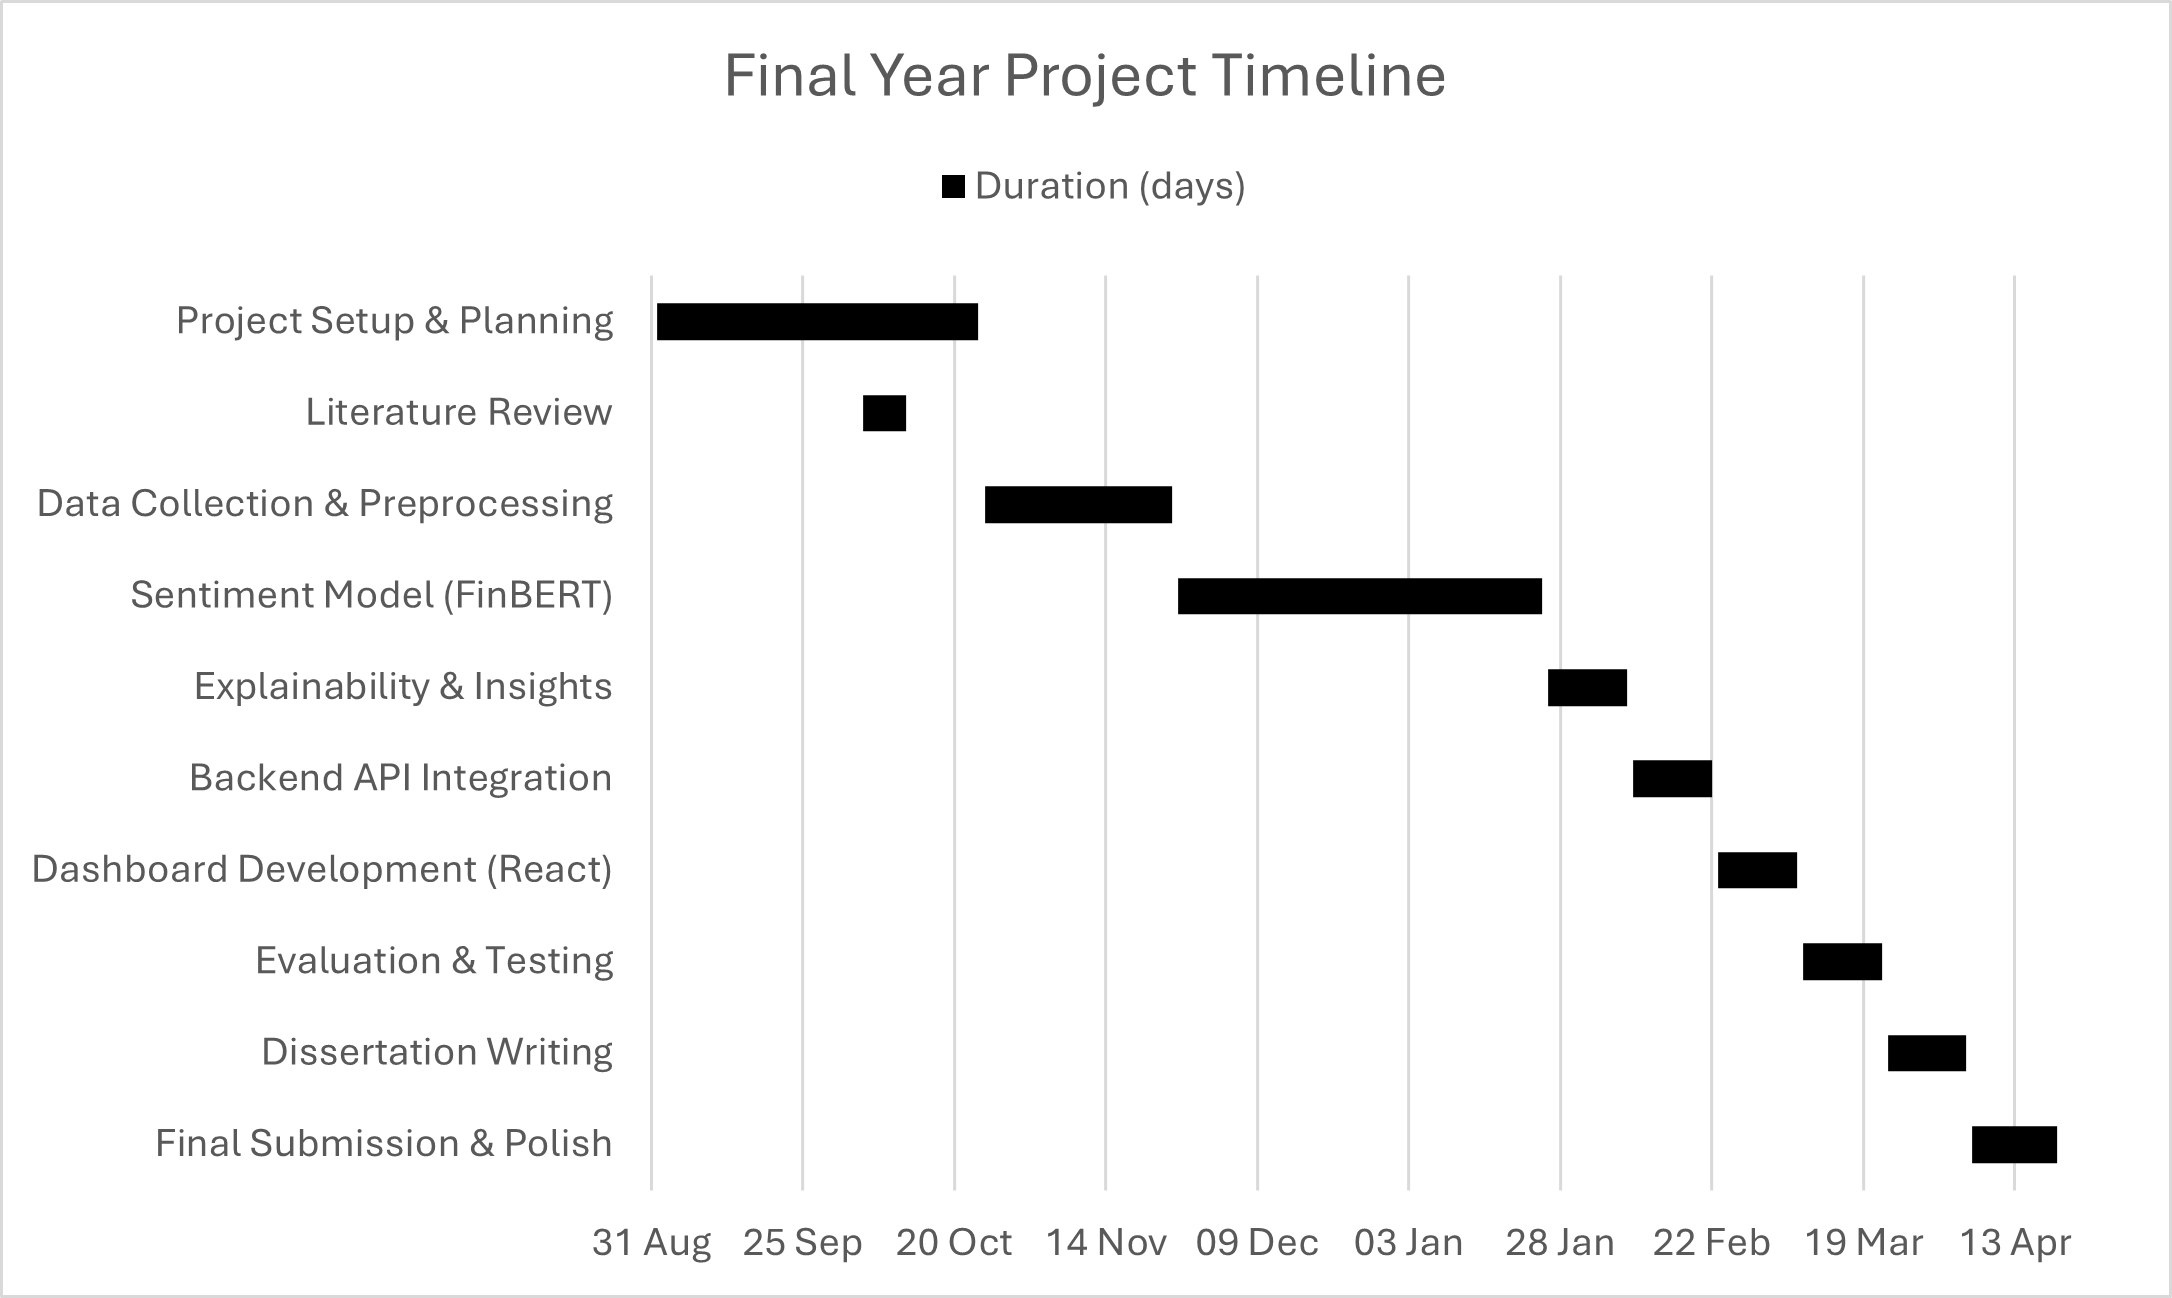
\includegraphics[width=\linewidth,height=0.92\textheight,keepaspectratio]{gantt_chart.png}%
    }{%
      \fbox{\parbox{0.88\linewidth}{\centering\vspace{1.5em}%
      Gantt chart image not found (\texttt{figures/gantt\_chart.png}).%
      \vspace{1.5em}}}%
    }
    \caption{Project workplan Gantt chart (September 2025--April 2026), updated at the January deliverable milestone.}
    \label{fig:gantt}
\end{figure}

\section{Ethics Awareness and Data Governance}
\label{app:ethics}

The project involved two distinct research activities, each with its own ethical classification.

\paragraph{Primary research: expert interviews.}
During the requirements and design phase (September--October 2025), a small number of structured interviews were conducted with finance and technology practitioners to understand how sentiment data is currently used in investment contexts and what features would make a sentiment dashboard genuinely useful. Participants were contacted via professional networks, informed of the academic purpose of the study, and their participation was entirely voluntary. No personally identifiable information was recorded; notes were taken with the assistance of an AI transcription tool (Notion AI) and are summarised in Appendix~\ref{app:interviews}. These interviews did not involve vulnerable populations, financial advice, or any form of compensation, and were therefore within the scope of the project's Ethics Awareness Form.

\paragraph{Secondary data: public text corpus.}
The Ethics Awareness Form (EAF) was completed with my supervisor in September 2025 and the primary data collection activity was classified as secondary use of publicly posted text: no surveys, no private messages, no paywalled content, and no attempt to re-identify individuals beyond information already publicly visible. The completed and signed EAF is included at the bottom of the approved Project Brief submitted in October 2025; this section summarises how those commitments were implemented in the codebase (see also Chapter~\ref{chap:system_design}).

\begin{itemize}
  \item Reddit: OAuth application registered; rate limits respected through exponential backoff and pagination.
  \item X/Twitter: official documented interfaces used where possible; unofficial pathways kept within modest volume bounds with automatic fallback.
  \item NewsAPI: API key stored only as an environment variable; never committed to the repository.
  \item Storage: database credentials kept exclusively in environment variables; lean deployment mode prevents accidental ML stack loading on public-facing instances.
\end{itemize}

\section{Representative Dataset Sample}
\label{app:dataset_sample}

Table~\ref{tab:dataset_sample} shows five representative rows from the ingested corpus. Text is truncated to fit the table; actual records contain full post or article text.

\begin{table}[!ht]
\centering
\small
\caption{Representative sample of five ingested records from the multi-source corpus.}
\label{tab:dataset_sample}
\begin{tabular}{@{}p{2.6cm} p{6.4cm} p{1.6cm} p{1.4cm}@{}}
\toprule
\textbf{Source} & \textbf{Text (truncated)} & \textbf{Label} & \textbf{Ticker} \\
\midrule
Reddit (WSB)     & NVDA earnings beat again; price action discussed in thread. & positive & NVDA \\
X (snscrape)     & Fed decision day: indices sold off hard into the close.    & negative & SPY  \\
NewsAPI          & Apple Q4 revenue above analyst expectations; shares higher. & positive & AAPL \\
Reddit (investing) & Bitcoin feels stretched here; unsure about adding.        & negative & BTC  \\
NewsAPI          & Mixed session as investors wait for CPI print tomorrow.    & neutral  & \textit{n/a} \\
\bottomrule
\end{tabular}
\end{table}

\section{Extended Evaluation Results}
\label{app:extended_results}

Table~\ref{tab:full_results_appendix} presents the full per-class results underlying the summary in Chapter~\ref{chap:evaluation} (Tables~\ref{tab:benchmark_summary} and~\ref{tab:per_class}). The bar chart and confusion-matrix heatmap in that chapter are Figures~\ref{fig:metrics_barchart} and~\ref{fig:cm_heatmap}.

\begin{table}[!ht]
\centering
\small
\caption{Full per-class evaluation results for FinBERT and the keyword baseline on the 200-sample benchmark (values are proportions).}
\label{tab:full_results_appendix}
\begin{tabular}{@{}llccc@{}}
\toprule
\textbf{Model} & \textbf{Class} & \textbf{Precision} & \textbf{Recall} & \textbf{F1} \\
\midrule
FinBERT & Positive  & 0.759 & 0.943 & 0.841 \\
        & Negative  & 0.825 & 0.943 & 0.880 \\
        & Neutral   & 0.970 & 0.533 & 0.688 \\
        & \textbf{Macro avg} & \textbf{0.851} & \textbf{0.806} & \textbf{0.803} \\
\midrule
Keyword baseline & Positive  & 0.809 & 0.786 & 0.797 \\
                 & Negative  & 0.750 & 0.471 & 0.579 \\
                 & Neutral   & 0.557 & 0.817 & 0.662 \\
                 & \textbf{Macro avg} & \textbf{0.705} & \textbf{0.691} & \textbf{0.679} \\
\bottomrule
\end{tabular}
\end{table}

\paragraph{Single-annotator note.}
Ground-truth labels were assigned by the author, cross-referenced against the Financial PhraseBank taxonomy \citep{malo2014financialphrasebank} for consistency. The absence of multi-annotator inter-rater reliability scores is acknowledged as a limitation; a crowdsourced re-annotation of a subset is identified as a priority for future work.

\section{Illustrative API Response Schemas}
\label{app:api_samples}

The following JSON fragments illustrate the response shapes returned by two key endpoints. Field names reflect the codebase conventions; exact keys may vary slightly by route version.

\subsection*{Sentiment Prediction}

\begin{lstlisting}[basicstyle=\ttfamily\footnotesize,breaklines=true,frame=single]
{
  "label": "positive",
  "scores": {"positive": 0.87, "neutral": 0.08, "negative": 0.05},
  "model": "ProsusAI/finbert",
  "source": "reddit"
}
\end{lstlisting}

\subsection*{LIME Explanation}

\begin{lstlisting}[basicstyle=\ttfamily\footnotesize,breaklines=true,frame=single]
{
  "tokens": ["Apple", "guidance", "was", "cautious"],
  "weights": [0.31, 0.22, -0.02, 0.09],
  "target_label": "negative",
  "latency_ms": 1840
}
\end{lstlisting}

\section{Environment Variables and Deployment Switches}
\label{app:env_table}

Table~\ref{tab:env_vars} lists the principal environment variables controlling ingestion backend selection and deployment mode.

\begin{table}[!ht]
\centering
\small
\caption{Principal environment variables for ingestion, Twitter backend selection, and lean API mode.}
\label{tab:env_vars}
\begin{tabular}{@{}p{4.6cm}p{8.4cm}@{}}
\toprule
\textbf{Variable} & \textbf{Role} \\
\midrule
\texttt{DATABASE\_URL}            & Connection string for the Neon PostgreSQL instance. \\
\texttt{NEWS\_API\_KEY}           & Authenticates NewsAPI requests. \\
\texttt{TWITTER\_INGEST\_BACKEND} & Selects \texttt{api}, \texttt{snscrape}, \texttt{csv}, or \texttt{auto}. \\
\texttt{TWITTER\_BEARER\_TOKEN}   & Enables the official X API v2 path when present. \\
\texttt{LEAN\_API}                & When set, inference-heavy routes return \texttt{503} instead of loading PyTorch. \\
\texttt{(CI secrets)}             & GitHub Actions supplies tokens and cache keys at runtime. \\
\bottomrule
\end{tabular}
\end{table}

\section{Expert Interview Summaries}
\label{app:interviews}

During the requirements phase of the project, three structured interviews were conducted with three separate finance and technology practitioners to validate the project's motivation and inform feature priorities. Two sessions took place on 13 October 2025 and a third on 21 October 2025; the interviews were conducted online, lasted approximately 60--70 minutes each, and were focused around three themes: (i) how investor sentiment is currently monitored in practice; (ii) what data sources are considered most reliable; and (iii) what analytical capabilities would make a sentiment dashboard genuinely useful to a practitioner. Table~\ref{tab:interview_sessions} lists the sessions.

\begin{table}[!ht]
\centering
\small
\begin{tabular}{@{}llp{6.8cm}@{}}
\toprule
\textbf{Date} & \textbf{Format} & \textbf{Scope of discussion} \\
\midrule
13 October 2025 (session 1) & Online, $\sim$70 min & Project scoping; sentiment tool landscape; market dynamics; ethics and commercialisation. \\
13 October 2025 (session 2) & Online, $\sim$60 min & Feature priorities; data-source reliability; manipulation and signal quality. \\
21 October 2025            & Online, $\sim$60 min & Follow-up on explainability requirements and commercialisation pathway. \\
\bottomrule
\end{tabular}
\caption{Expert interview sessions conducted during the requirements phase (three interviewees in total, one per session).}
\label{tab:interview_sessions}
\end{table}

Participants were three practitioners whose combined experience spans investment management, financial compliance, blockchain and fintech, software entrepreneurship, and financial-crime cybersecurity. In keeping with the project's ethics classification, all material below is anonymised: no participant names, employer names, or identifying details are retained.

\paragraph{Key themes from the interviews.}
The three sessions produced substantially overlapping insights, which are consolidated here thematically rather than reported session-by-session.

\begin{itemize}
  \item \textbf{Existing tool gap.} Practitioners described existing sentiment tooling (e.g.\ Brandwatch) as effective for brand and product sentiment but weaker for financial markets, and typically priced or positioned for enterprise use rather than individual investors. This directly supported the project's framing of an accessible, finance-specific sentiment dashboard as a genuine gap.
  \item \textbf{Source manipulation and signal quality.} Participants were emphatic that social-media data is routinely shaped by bots, coordinated influence campaigns, and algorithmic feed curation controlled by a small number of platforms. They recommended explicit multi-source comparison rather than reliance on any single feed, and flagged bot/inauthenticity filtering as an important future capability. This reinforced the multi-source ingestion design (Chapter~\ref{chap:system_design}) and motivates a dedicated future-work item (Chapter~\ref{chap:conclusion}).
  \item \textbf{Explainability and trust.} The ability to see \emph{why} a text received a particular label was raised independently across the sessions as important for building practitioner trust in automated sentiment. This directly shaped the decision to expose LIME explanations through the API and render them as a token-level heatmap in the UI.
  \item \textbf{Market regime context.} Practitioners observed that recent markets have been partially decoupled from fundamentals by post-2008 quantitative easing and asset-price inflation, which weakens purely technical signals and makes behavioural and sentiment indicators comparatively more interesting. This informs the interpretive caveats applied to the correlation analysis in Chapter~\ref{chap:discussion}.
  \item \textbf{Commercialisation pathway.} When prompted, the participants advised an MVP-first approach: ship a minimal useful version, obtain practitioner feedback, and iterate, rather than attempting to pre-engineer a complete product. This framing shaped the scope boundary between the submitted academic system and the longer-term productisation pathway (see the industry demonstration and future-work sections in Chapter~\ref{chap:conclusion}).
  \item \textbf{Wider AI outlook.} Participants also observed that large language models are already writing a substantial share of production code at major firms and will continue to reshape both financial services and labour markets over the next several years. This is treated as contextual colour for the Discussion chapter rather than as a formal finding of the project.
\end{itemize}

\paragraph{Interview notes and recording status.}
Notes were taken during the first session on 13 October 2025 with AI transcription assistance (Notion AI) and are available on request. Recordings for the second 13 October 2025 session and the 21 October 2025 session did not export successfully, so those sessions are represented here only through contemporaneous hand-written notes; the themes above were consistent across all three sessions, which is why they are reported in consolidated form. No personally identifiable information was retained in any case. The interviews are cited here as context for the requirements process rather than as formal qualitative data.


% ==========================================================
% END OF DOCUMENT
% ==========================================================
\end{document}
